\documentclass[a4paper,nofonts,justified,colorinlistoftodos,hidelinks]{tufte-book}

\usepackage[T1]{fontenc}
\usepackage[utf8]{inputenc}
\usepackage[english]{babel}

\usepackage[a-2u]{pdfx}

\usepackage{graphicx}
\usepackage{algorithmicx}
\usepackage{algpseudocode}
\usepackage{algorithm}
\usepackage{color}
\usepackage{tikz}
\usepackage{pgfplots}
\usepackage{makeidx}
\usepackage{amssymb}
\usepackage{amsthm}
\usepackage{amsmath}
\usepackage{booktabs}
\usepackage{tensor}

\usepackage{todonotes}

\usepackage{libertine}
\usepackage{mathpazo}
\usepackage[scaled=0.83]{beramono}
\usepackage{microtype}
\usepackage{xfrac}
\usepackage{xspace}

\usetikzlibrary{fit}

\graphicspath{{./graphics/}}
 
%!TEX root = main.tex

%math definitions
\newcommand{\Real}{{\ensuremath{\mathbb{R}}}}
\newcommand{\Nat}{\mathbb{N}\xspace}
\newcommand{\Int}{\mathbb{Z}\xspace}
\newcommand{\Rat}{\mathbb{Q}\xspace}
\newcommand{\dom}{\mathrm{dom}}
\newcommand{\rng}{\mathrm{rng}}
\newcommand{\restrict}{\upharpoonright}
\newcommand{\idr}{\mathrm{Id}}
\newcommand{\normal}[2]{\mathcal{N}(#1, #2)}
\newcommand{\uniform}[2]{\mathcal{U}(#1, #2)}
\newcommand{\charf}{1}
\newcommand{\identity}{\mathrm{I}}
\newcommand{\setdiff}{\bigtriangleup}
\newcommand{\powerset}{\mathcal{P}}

\newtheorem{theorem}{Theorem}


\newcommand{\twopartdef}[4]
{
	\left\{
		\begin{array}{ll}
			#1 & \text{pro } #2 \\
			#3 & \text{pro } #4
		\end{array}
	\right.
}
\newcommand{\twopartdefotherwise}[4]
{
	\left\{
		\begin{array}{ll}
			#1 & \text{pro } #2 \\
			#3 & \text{jinak} #4
		\end{array}
	\right.
}

\newcommand{\informal}[1]{\smallskip\noindent\colorbox{SkyBlue}{\begin{minipage}{\textwidth-6pt}
  \textbf{Informal! }#1
\end{minipage}}\smallskip}

% todos, comments, ...
\newcommand{\pozn}[1]{\todo[inline,color={CornflowerBlue},size=\small]{\sc{#1}}}
\newcommand{\missingref}{\todo[color={WildStrawberry}]{\textbf{Missing ref.}}}
\newcommand{\add}[1]{\todo[inline, color={YellowGreen}]{#1}}
\newcommand{\ask}[1]{\todo[inline, color={Peach}]{\textbf{???} #1}}
\newcommand{\redo}[1]{\todo[inline, color={BurntOrange}]{\textbf{<!>} #1}}

\newcommand{\code}[1]{\texttt{#1}}


% mathematical notation

\makeatletter
\renewcommand{\maketitlepage}{%
\begingroup%
\setlength{\parindent}{0pt}

%\includegraphics[width=\textwidth]{graphics/logotyp_fakulty1}

\vspace{5in}{\fontsize{36}{54}\selectfont\@title\par}
\vspace{0.5in}{\fontsize{24}{24}\selectfont\textit{\@author}\par}
\vspace{0.25in}{\fontsize{16}{16}\selectfont\textit{Based on lectures by Petr Gregor}\par}


\vfill{\fontsize{14}{14}\selectfont\textsf{\smallcaps{\@date}}\par}


\thispagestyle{empty}
\endgroup
}
\makeatother

\makeindex

\frontmatter

\title{Lecture Notes on \\ Propositional and \\ Predicate Logic}
\author{Martin Pilát}
\date{\today}

\begin{document}

\maketitle

\mainmatter

%!TEX root = main.tex

\chapter{Introduction}

Generally, logic is a study of arguments and inferences. While it started as philosophical discipline in ancient times, it is now widely studied in mathematics and computer science. As such, logic provides the basic language and tools for most of mathematics. It studies different prove systems and discusses whether they are sound (everything they prove is valid) and complete (everything that is valid can be proven). 

While logic provides rather low-level tools for mathematics and computer science, it still has rather wide applications. For example, in some areas of artificial intelligence, logic is used to represent the knowledge of the intelligent agents and reason about it. The agents then use logical reasoning (theorem proving) to decide what to do next, or prove that a certain action is safe in a given environment. Another important area is formal software verification, where logic (and, again, theorem proving) can be used to formally verify, that a program indeed does what it should according to a specification. This is essential while implementing e.g. cryptographic protocols. Formal verification is also used while designing digital circuits.

There are also attempts to formalize the whole mathematics in logic and use computers to check that all the proofs are correct. For example, Mizar\sidenote{\url{http://www.mizar.org/library/}} is a system that aims to re-create most of the mathematics with formal and verified proofs. The verification starts from the basic mathematical axioms -- in the case of the Mizar system, authors of so called Mizar articles can use only axioms of set-theory and theorems from previously verified articles. Therefore, everything published in the Mizar mathematical library is verified to be a correct consequence of the base axioms.

Logic serves as the formal language of mathematics, and therefore logic also needs to formally specify the syntax of the language. The syntax defines, what is a valid logical formula and what is not, however the meaning and validity of a formula is given by the semantics of the language. Logic itself prescribes the meaning of only a handful of symbols -- namely the logical connectives ($\land, \lor, \to, \leftrightarrow, \neg$) and the quantifiers ($\forall, \exists $). Additionally, in languages with equality, the meaning of ``$=$'' is also given. All other symbols used in logical formulas can have arbitrary meaning, which is given by the semantics. So, for example, if we write a formula $(\forall x)(\forall y)(x + y = y + x)$, we cannot discuss its validity before defining the meaning of ``$+$''. The formula is valid if we are talking about the real numbers and ``$+$'' denotes their addition, however, the symbol ``$+$'' can also represent (quite unusually) the multiplication of square matrices, and in such a case, the formula is not valid.

There are different levels of the language of logic. In propositional logic, only propositional variables (those that are either true or false) and the logical connectives can be used. In first order logic, we can additionally use functions, relations and quantifiers for variables that range objects from some universe. In second order logic, there are additionally quantifiers for sets of objects in the universe (and, more specifically, for functions and relations). In higher order logic, we also have variables for sets of sets of objects. For example, a formula in propositional logic $$ (d \land c) \to s$$ can express that if it is dark and clear outside, the stars are visible. In a first order language, we can have a more complex formula $$ (\forall x)(\forall y)(S(x) \land E(y) \to (L(x,y) \to P(x, y)))$$ that expresses that if $x$ is a student ($S(x)$) and $y$ is an exam ($E(y)$), if $x$ learns for $y$ ($L(x,y)$) then $x$ passes $y$ ($P(x,y)$). As an example of second order language, we can write the axiom of induction: $$ (\forall P)(P(0) \land (\forall n)(P(n) \to P(n+1)) \to (\forall n)P(n))\,.$$

In the lecture, we will deal mostly with propositional and first-order logic, however there are also other extension of logic. For example, in multi-agent systems, so called modal logic is often used to represent the knowledge. In modal logic, there are special modalities, that can further qualify a statement. For example, there is a modality that says that a statement may be true, or must be true. Other types of modal logic contain modalities that express knowledge of other agents (e.g. ``agent $A$ knows that statement $S$ is true'' can be written as $\mathrm{K}_A.S$, or even ``agent $A$ knows that agent $B$ knows that statement $S$ is true'' ($\mathrm{K}_A.\mathrm{K}_B.S$)). Another interesting type of modal logic is temporal logic, which contain modalities about time and can express e.g. ``statement $S$ will be true sometimes in the future''.

\section{About these lecture notes}

In these lecture notes, logic is presented for students of computer science. Therefore, focus is given to areas most needed for computer scientists. For example, we use the more intuitive tableau method instead of the Hilbert-style prove systems. We also explain the resolution method in logic as a background to Prolog and logical programming. The more advanced topics on decidability and incompleteness are explained in a more informal way.

You are currently reading the first version of the lecture notes, which can, and most probably will, contain some errors. If you find an error, or if something is not clear, do not hesitate to contact the author by e-mail\sidenote{\url{Martin.Pilat@mff.cuni.cz}}, or, alternatively, create an issue in the GitHub repository of the book\sidenote{\url{https://github.com/martinpilat/logic-book}}. 

There are also other resources you may want to check. One of them are the presentations created by Petr Gregor for his version of the lecture\sidenote{\url{http://ktiml.mff.cuni.cz/~gregor/logics/index.html}}, that serve as a base for these lecture notes.

\informal{The author of these notes sometimes likes to explain things in a more intuitive way with some not-so-formal examples and metaphors. While he  believes these can help to get better understanding of the given concept, they sometimes (read ``often'') are rather informal and have some limitations. Therefore, in these notes, they will be set in boxes like the one you are reading just now with a bold ``\textbf{Informal!}'' warning. The information contained in these boxes is always non-essential to the rest of the text and can be (some would even argue that should be) skipped.}

\section{Preliminaries}

Like many mathematical texts, these lecture notes also assume that the reader has some basic knowledge. The most important concepts (many of which should sound familiar) are briefly introduced in this short section, both to provide a single place where these can be found and to introduce the notation used in these lecture notes.

We will start with the basic set-theoretic notions. The most basic of these is the \emph{class}. Each property of sets $\varphi(x)$ defines a class $\{x|\varphi(x)\}$. Some classes are also sets, those that are not are called \emph{proper classes}. The distinction between sets and classes is probably new for most of the readers. Why would we need any other collections of objects than sets? How is it possible, that there is a collection of objects, which is not a set? The reason to distinguish between these two is that if everything was considered a set, we could find paradoxes in the set theory. For example, if we had a set of all sets that do not contain themselves, does this set contain itself, or not? Let us assume, it does, but then, by definition, it does not. If we instead assume it does not contain itself, then, again, by definition, it does. This so called Russel's paradox can be avoided by using a notion of classes, that cannot contain other classes. 

\informal{A class can be understood as any collection of sets that can be described by the language of set theory. However, some of these collections do not make much sense and can lead to paradoxes. Therefore, any collection, that would lead to some paradox is denoted as a proper class instead of a set and the paradoxes can thus be avoided.}

The other set-theoretic notions should be much more familiar. We use $x \in y$ to denote that $x$ is a member of set $y$, $x \notin y$ and $x \neq y$ are shortcuts for $\neg (x \in y)$ and $\neg (x = y)$. A set containing exactly elements $x_0, x_1, \dots, x_n$ is denoted as $\{x_0, x_1, \dots, x_n\}$. A set with only one element $\{x\}$ is called a \emph{singleton} and a set with two elements $\{x_0, x_1\}$ is called an \emph{unordered pair}. We will also use the common notation for set operations: $\emptyset$ denotes an \emph{empty set}, $\cup$ and $\cap$ denote \emph{union} and \emph{intersection} of sets. The $\setminus$ is the \emph{set difference} operator and $\setdiff$ is the \emph{symetric set difference} operator $$x \setdiff y = (x \setminus y) \cup (y \setminus x)\,.$$

Two sets are \emph{disjoint}, if their intersection is an empty set, and $x \subseteq y$ denotes that $x$ is a subset of $y$ (all elements of $x$ are also elements of $y$). The set of all subsets of a set $x$ -- the \emph{power set of $x$} -- is denoted as $\mathcal{P}(x)$. The \emph{union of set $x$}, $\bigcup x$, is the union of all sets contained in $x$. A \emph{cover of a set $x$} is a set $y \subseteq \mathcal{P}(x) \setminus \emptyset$, such that $\bigcup y = x$, if all the sets in the cover $y$ are mutually disjoint, than $y$ is a \emph{partition of $x$}.

The definition of an unordered pair can be used to define the \emph{ordered pair} $(a, b) = \{a, \{a,b\}\}$ and an \emph{ordered $n$-tuple} $(x_0, \dots, x_{n-1}) = ((x_0, \dots, x_{n-2}), x_{n-1})$ for $n > 2$. A Cartesian product of two sets $a$ and $b$ is $a \times b = \{(x,y) | x \in a, y \in b\}$ and the Cartesian power of a set $x$ is $x^0 = \{\emptyset\}$, $x^n = x^{n-1} \times x$. A \emph{binary relation} $R$ is a set of ordered pairs. The \emph{domain of $R$} is defined as $\dom(R) = \{x|(\exists y)(x,y)\in R\}$, the \emph{range of $R$} is similarly $\rng(R) = \{y|(\exists x)(x,y)\in R\}$. The \emph{extension of $x$ in $R$} is the set $R[x] = \{y|(x,y)\in R\}$. The symbol $R^{-1}$ denotes the \emph{inverse relation} $R^{-1}=\{(y,x)|(x,y)\in R\}$. The \emph{restriction of $R$ to a set $z$} is defined as $R \restrict z = \{(x,y) \in R|x \in z\}$. Two relations can also be \emph{composed} into one, $R \circ S = \{(x,z)|(\exists y)((x,y) \in R \land (y,z) \in S\}$. The \emph{identity relation} on set $z$, $\idr_z = \{(x,x)|x\in z\}$. 

A binary function $f$ is a special type of binary relation where for every $x \in dom(f)$ there is exactly one $y$ such that $(x,y) \in f$, then, $y$ is the value of $f$ in $x$ denoted as $f(x)$. $f: X \to Y$ denotes a function $f$ with $\dom(f) = X$ and $\rng(f) \subseteq Y$. The set of all such functions is $^YX$. A function $f: X \to Y$ is a \emph{surjection} (onto) if $\rng(f)=Y$, and it is an \emph{injection} (one-to-one) if for any $x,y \in dom(f)$, $x \neq y \to f(x) \neq f(y)$. A function that is both a surjection and injection is called a \emph{bijection}. Similarly to relation, we can define the inverse function $f^{-1}$, and the composition of functions $f:X\to Y$ and $g:Y\to Z$ as a function $f \circ g$ with $(f \circ g)(x) = g(f(x))$. The image of a set $A$, denoted as $f[A]$ is the set of function values for all elements of $A$, $f[A] = \{y |(x,y) \in f, x \in A\}$.

There are also two special types of relations which will be important later: equivalences and orders. An equivalence on a set $X$ is relation that is reflexive ($R(x,x)$ for all $x\in X$), symmetric ($R(x,y) \to R(y,x)$ for $x,y \in X$) and transitive ($(R(x,y) \land R(y,z)) \to R(x,z))$ for all $x,y,z \in X$). The extension of $x$ in $R$ is called the equivalence class of $x$ and is also denoted as $[x]_R$. $X/R = \{R[x] | x \in X\}$ is the \emph{quotient set of $X$ by $R$}. The quotient set is always a partition of $X$ and every partition of $X$ also defines an equivalence on $X$ (two elements are equivalent if they are in the same set in the partition). 

The other important types of the relations are the orders, usually an order is denoted as $\leq$. Such a relation is a \emph{partial order of a set $X$}, if it is reflexive ($x \leq x$ for $x \in X$), antisymmetric ($x \leq y \land y \leq x \to x = y$ for $x,y\in X$) and transitive ($x \leq y \land y \leq z \to x \leq z$ for $x,y,z \in X$). If, additionally, for every two elements $x,y \in X$ it holds that $x \leq y$ or $y \leq x$ (dichotomy) than $\leq$ is a total (linear) order. It is a well-order if additionally every non-empty subset of $X$ has a least element. Finally, an order of $X$ is dense, if $X$ is not a singleton and for every two elements $x,y \in X$, there is another element $z \in X$ between these two ($x < y \to (\exists z) (x < z \land z < y))$, where $a < b$ means that $a \leq b \land a \neq b$. 

For example, the common ordering of natural numbers ($\leq$ on $\Nat$) is a linear well-order (as every two natural numbers are comparable and every subset of natural numbers has a least element under this order), however, it is not a dense order, as for example there is no natural number between 0 and 1. On the other hand, the common ordering of rational numbers is a dense linear order (there is a rational number between any pair of distinct rational numbers), however it is not a well-order, as e.g. the set $\{x \in \Rat\ | x \leq 0\}$ has no least element.

The natural numbers can be defined using the empty set in an inductive way -- $0 = \emptyset\,,1=\{0\} = \{\emptyset\}\,, 2=\{0,1\} = \{\emptyset, \{\emptyset\}\}\,, \dots, n=\{0, \dots, n-1\}, \dots\,.$ The set of all natural numbers $\Nat$ is the smallest set containing $\emptyset$ and closed under the operation of successor $S(x) = x \cup \{x\}$. The other common sets of numbers are the integers, which can be defined as the $\Int = (\Nat \times \Nat)/\sim\,,$ with $(a,b) \sim (c,d)$ if and only if $a + d = b + c\,.$ Similarly, the set of rational numbers $\Rat$ can be defined as $\Rat = (\Int \times (\Int \setminus \{0\}))/\sim\,,$ with $(a,b) \sim (c,d)$ if and only if $ad=bc$. The definition of real numbers $\Real$ is more complex. These are usually defined as cuts of the rational numbers $\Rat$, where a cut is a partition of $\Rat$ into two sets $A$ and $B$, where all numbers in $B$ are greater than all numbers of $A$, and $A$ has no greatest element. For example, the cut corresponding to the irrational number $\sqrt{2}$ is $A = \{a\in \Rat | a^2 < 2 \lor a < 0\}\,, B = \{b\in \Rat | b^2 > 2 \land b > 0\}\,.$

Another important notion for the rest of the lecture deals with the cardinality (``size'') of sets. A set $X$ has a cardinality smaller or equal to the cardinality of a set $Y$ ($X \preceq Y$) if there is an injective function $f: X \to Y$. If there is a bijection $f: X \to Y$ then we say that $X$ and $Y$ have the same cardinality ($X \approx Y$), finally $X$ has strictly smaller cardinality than $Y$ ($X \prec Y$) if ($X \preceq Y \land \neg(X \approx Y)$). For each set $x$, there is a cardinal number $\kappa \approx x$, denoted as $|x| = \kappa$. A set $X$ is \emph{finite} if $|X| = n$ for some $n \in \Nat$. It is \emph{countable}, if it is finite or if $|x| = |\Nat| = \omega$. Otherwise, it is \emph{uncountable}. The cardinality of $\mathcal{P}(\Nat)$ is called the continuum.

It is interesting to know the cardinality of the common sets of numbers. Obviously, the set of natural numbers $\Nat$ is countable. A less obvious fact is that the sets of integers and rational numbers also have the same cardinality and are therefore also countable. For the integers, we can create an infinite sequence of integers $s = \langle 0, 1, -1, 2, -2, 3, -3, \dots \rangle$, then a function $f(i) = s_i$ is an injective function $\Nat \to \Int$, therefore $\Int \preceq \Nat$. The other inequality ($\Nat \preceq \Int$) is obvious (use identity as the injective function). In order to show that the set of rational numbers $\Rat$ is also countable, we can create a function $f(\frac{p}{q}) = 2^{|p|}3^q5^{\mathrm{sign}(p)}$ (we consider only cases where $p \in \Int, q \in \Nat \setminus \{0\}$, which clearly covers all the rationals), this is again an injective mapping $\Rat \to \Nat$ and therefore $\Rat \preceq \Nat$. As before, the other inequality is trivial. Finally, we can show that the set of real numbers $\Real$ has bigger cardinality than the set of natural numbers $\Nat$. Obviously $\Nat \preceq \Real$ as $\Nat \subseteq \Real$. Let us assume both the sets have the same cardinality, in such a case there is bijection $f: \Nat \to \Real$. We will now define a new real number $r$ in the following way. The integer part of the number is 0, the first digit after the decimal point is different from the first digit after decimal point in $f(0)$, the second digit is different from the second digit in $f(1)$, and so on\sidenote{If we write the decimal value of the number $r$ as $r = 0.r_0r_1r_2\dots$, where $r_i$ is the $i$-th decimal digit, we can define $r_i = (f(i)_i + 1)\, \mathrm{mod}\, 10$, where $f(i)_i$ is the $i$-th decimal digit of $f(i)$.}. This real number is different from all the numbers in $\{f(0), f(1), \dots\}$ as it differs from the number $f(i)$ in the $i$-th digit after the decimal point. This is a contradiction with the assumption that $f$ is a bijection between $\Nat$ and $\Real$ and therefore $\Nat \prec \Real$.

We will conclude the discussion of cardinalities by showing the Cantor's theorem.

\begin{theorem}[Cantor]
For every set $x$, $x \prec \powerset(x)$.
\end{theorem}

\begin{proof}
First, $f(x) = \{x\}$ is an injection $X \to \powerset(x)$ and therefore $x \preceq \powerset (x)$. Suppose there is also an injective $g: \powerset (x) \to x$. We can define a set $y = \{g(z)|z \subseteq x \land g(z) \notin z\}$. Now, similarly to the Russel's paradox, $g(y) \in y$ if and only if $g(y) \notin y$, which is a contradiction, and therefore there cannot be any such injective $g$ and so $x \prec \powerset(x)$.
\end{proof}

As the tableau method used in this lecture relies on trees, we will conclude this preliminary section by a brief discussion on trees. Most of the readers are probably familiar with finite trees, however, we will sometimes need to work with infinite trees and therefore we define a \emph{tree} as a set $T$ with a partial order $<_T$ (called the tree order) with a unique least element (\emph{the root}) and in which the set of predecessors of any element is well-ordered by $<_T$. In this definition a branch is a maximal linearly ordered subset of $T$. Apart from this difference in definition, we will use the common terminology on trees from the graph theory. For simplicity, we will only consider finitely branching trees, where each node except the root has an immediate predecessor\sidenote{This means, we will not deal, for example, with trees where the nodes would be set of rational numbers $\Rat$ and the tree order $<_T$ would be the common order on $\Rat$.}. In such trees we can define the \emph{levels of the tree}. The root is on the level 0, the sons of the nodes on the $(n-1)$-th level are on level $n$. The depth of tree is maximal $n \in \Nat$ of a non-empty level. In case the tree has an infinite branch it has an infinite depth $\omega$. In an $n$-ary tree, each node has at most $n$ sons and a tree is finitely branching if each node has a finite number of sons.

\begin{lemma}[König]
Every infinite, finitely branching tree contains an infinite branch.
\end{lemma}
\begin{proof}
The root of the tree has only finitely many sons, therefore there is a son of the root that is infinite. We choose this son and continue in the same way with his sons, thus constructing an infinite branch.
\end{proof}

Apart from the tree order $<_T$ we sometimes need to work with \emph{ordered trees} where the sons of each node are additionally ordered from left to right with a \emph{left-to-right order} $<_L$. In a \emph{labeled tree} each node also contains an additional information. For example, the formula $$(p \land q) \to q$$ can be represented as the labeled ordered tree on the right.

\begin{marginfigure}[-4\baselineskip]
\centering
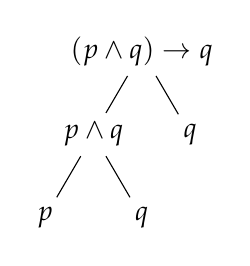
\begin{tikzpicture}[sibling distance=3.5em, level distance=3em]
  \node {$(p \land q) \to q$}
    child { node {$p \land q$} 
      child {node {$p$}}
      child {node {$q$}} }
    child { node {$q$} };
\end{tikzpicture}
\caption{The labeled ordered tree representing the formula $(p \land q) \to q$.}
\end{marginfigure}

\part{Propositional Logic}

%!TEX root = main.tex

\chapter{Propositional Formulas and Models}

In this chapter, we start the discussion of propositional logic. We will define, how propositional formulas look, what is a model in propositional logic and we will also discuss some special forms of formulas.

Propositional logic is the more basic type of logic (and predicate logic is an extension of propositional logic in a sense).  Propositional formulas (propositions) are created from so called \emph{propositional variables} that represent an atomic fact which can either be true or false. These propositional variables can only be connected by common logic connectives ($\to$, $\lequiv$, $\land$, $\lor$, $\neg$). Logical formulas can additionally use parentheses to indicate the order of application of connectives. While the propositional formulas are simple compared to formulas in other types of logic, they are still useful. One of the most important problems in propositional logic and in computer science in general is the satisfiability of propositional formulas (SAT). Many other NP-complete problems are often solved by transformation to the SAT problem and using one of the existing SAT solvers.

\section{Syntax of Propositional Logic}

The set of propositional variables is often called $\Prop$ and the variables themselves are usually named $p, q, r, s$ or $p_0, p_1, \dots, q_0, q_1$, or similarly. Now, we can formally define the propositional formula (over $\Prop$).

\begin{definition}
Let $\Prop$ is the set of propositional variables, than
\begin{enumerate}
  \item Every propositional variable from $\Prop$ is a propositional formula.
  \item If $\varphi$ and $\psi$ are propositional formulas, then $(\varphi \to \psi), (\varphi \land \psi), (\varphi \lor \psi), (\varphi \lequiv \psi)$, and $(\neg \varphi)$ are propositional formulas.
  \item Every propositional formula is created by finite application of the two rules above.
\end{enumerate}
\end{definition}

The last part of the definition ensures that every formula is finite, this also means that each formula can contain only a finite number of distinct variables. The set of propositional variables used in a formula $\varphi$ will be denoted as $\Var(\varphi)$. On the other hand, the set of all propositional formulas using only variables from a set $\Prop$ will be denoted as $\VF_\Prop$.

Formulas are thus strings created from propositional variables, logical connectives, and parentheses, that fulfill the conditions in the definition above. A substring of such a string that also fulfills the conditions is called a \emph{sub-formula}. 

The formal definition of formula dictates the use of parentheses around every sub-formula, which can be rather cumbersome. Therefore, we define priorities of the logical connectives and can thus omit some of the parentheses. The standard priorities are such, that the negation ($\neg$) has the highest priority (therefore parentheses around $(\neg \varphi)$ can always be omitted), conjunction and disjunction ($\lor, \land$) have ``middle'' priority, and implication and equivalence ($\to, \lequiv$) have the lowest priority. Therefore, we can write $\varphi \land \psi \to \neg \varphi \lor \xi$ instead of $((\varphi \land \psi) \to ((\neg \varphi) \lor \xi))$. 

Each formula can be also represented by a so called \emph{formation tree}, which is a finite ordered tree, whose nodes are labeled with propositions -- the leaves are labeled with propositional variables, if a node has label $(\neg \varphi)$, it has a single son labeled with $\varphi$, and if a node has label $(\varphi \to \psi), (\varphi \land \psi), (\varphi \lor \psi),$ or $(\varphi \lequiv \psi)$, it has two sons, the left one has label $\varphi$, and the right one has label $\psi$. For example, a formula $p \land q \to \neg (p \lor s)$ is represented by the formation tree on the left.
\begin{marginfigure}[-4\baselineskip]
\centering
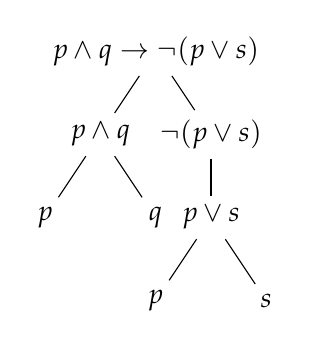
\begin{tikzpicture}[sibling distance=4em, level distance=3em]
  \node {$p \land q \to \neg (p \lor s)$}
    child { node {$p \land q$} 
      child {node {$p$}}
      child {node {$q$}} }
    child { node {$\neg (p \lor s)$}
    	child {node {$p \lor s$}
    		child {node {$p$}}
      	child {node {$s$}}}
     };
\end{tikzpicture}
\caption{The formation tree representing the formula $p \land q \to \neg (p \lor s)$.}
\end{marginfigure}

It is simple to show (by the induction on the number of nested parentheses) that each formula is associated with a unique formation tree. 

\section{Semantics of Propositional Logic}

Once we have the formal definition of the formula (the syntax of propositional logic), we can define its semantics (what the formula means). The propositional variables represent atomic statements, that can have one of two truth values -- either 0 (false) or 1 (true). The truth value of the whole proposition in then given by the truth values of the variables and by the semantics of the logical connectives, which is given in Table~\ref{tab:prop_semantics} bellow.

\begin{table}[h]
\centering
\caption{The semantics of logical connectives}
\label{tab:prop_semantics}
\begin{tabular}{cc|ccccc}
\toprule
$p$ & $q$ & $\neg p$ & $p \lor q$ & $p \land q$ & $p \to q$ & $p \lequiv q$ \\
\midrule
0 & 0 & 1 & 0 & 0 & 1 & 1 \\
0 & 1 & 1 & 1 & 0 & 1 & 0 \\
1 & 0 & 0 & 1 & 0 & 0 & 0 \\
1 & 1 & 0 & 1 & 1 & 1 & 1 \\
\bottomrule
\end{tabular}
\end{table}

We can also consider the table above a definition of Boolean functions $\lor_1, \land_1, \to_1, \lequiv_1,$ and $-_1$, that implement the logical connectives. We will use these functions in cases where it is needed (e.g. while talking about truth values of propositions). More generally, any propositional formula with $n$ variables defines a Boolean function $f: \{0,1\}^n \to \{0,1\}$ (later, we will also see that any Boolean function can be expressed using a propositional formula).

We also define two special logical formulas. The formula $\top \equiv p \lor \neg p$, which is always true, and the formula $\bot \equiv p \land \neg p$ which is always false.

We can now define the truth assignment and the truth value of formula more formally.

\begin{definition}
A \emph{truth assignment} is a function $v: \Prop \to \{0,1\}$, that is $v \in \fset{\Prop}{2}$.

A \emph{truth value} $\bar{v}(\varphi)$ of a propositional formula $\varphi$ for a truth assignment $v$ is defined inductively as:
	\begin{itemize}
		\begin{minipage}{0.5\textwidth}
		\item $\bar{v}(p) = v(p)$ if $p \in \Prop$
		\item $\bar{v}(\neg \varphi) = -_1(\bar{v}(\varphi))$ 
		\item $\bar{v}(\varphi \lor \psi) = \lor_1(\bar{v}(\varphi),\bar{v}(\psi))$ 
		\end{minipage}
		\begin{minipage}{0.5\textwidth}
		\item $\bar{v}(\varphi \land \psi) = \land_1(\bar{v}(\varphi),\bar{v}(\psi))$ 
		\item $\bar{v}(\varphi \to \psi) = \to_1(\bar{v}(\varphi),\bar{v}(\psi))$ 
		\item $\bar{v}(\varphi \lequiv \psi) = \lequiv_1(\bar{v}(\varphi),\bar{v}(\psi))$ 
		\end{minipage}
	\end{itemize}
\end{definition}

We can easily show (by the induction on the structure of the formula) that the truth value of a formula $\varphi$ depends only on the truth assignment of variables from $\Var(\varphi)$.

A proposition $\varphi$ over $\Prop$ is \emph{true in (satisfied by) an assignment} $v\in \fset{\Prop}{2}$, if $\bar{v}(\varphi) = 1$. In such a case, $v$ is called a \emph{satisfying assignment} for $\varphi$, we denote this fact $v \vDash \varphi$. If the formula is true for all assignments $v \in \fset{\Prop}{2}$, we say that it is \emph{valid (a tautology)} and denote the fact as $\vDash \varphi$. On the other hand, if there is no assignment for which the formula is true, it is called \emph{unsatisfiable (a contradiction)}. A formula $\varphi$ is \emph{independent (a contingency)} if it is neither a tautology nor a contradiction, i.e. there are two assignments $v_1, v_2 \in \fset{\Prop}{2}$, such that $\bar{v}_1(\varphi) = 1$ and $\bar{v}_2(\varphi) = 0$. Finally, a formula is \emph{satisfiable} if there is a truth assignment in which it is true.

A truth assignment of $\Prop$ is also called a model of the language $\Prop$. The set of all models of $\Prop$ is denoted as $M(\Prop)$, and, obviously $M(\Prop) = \fset{\Prop}{2}$. A proposition $\varphi$ over $\Prop$ is valid in a model $v \in M(\Prop)$, if $\bar{v}(\varphi) = 1$. Then we also say that $v$ is a model of $\varphi$, denoted as $v \vDash \varphi$. $M^\Prop(\varphi) = \{v \in M(\Prop) | v \vDash \varphi\}$ is the \emph{class of all models} of $\varphi$. A formula is valid, if it is true in every model of the language, it is unsatisfiable if it does not have a model, and satisfiable if it has a model. It is independent if it is true in a model of the language and false in another one. Formulas $\varphi$ and $\psi$ are logically equivalent ($\varphi \sim \psi)$, if $M^\Prop(\varphi) = M^\Prop(\psi)$.

The last two paragraphs say basically the same, the difference is that in the latter one, we use the notion of model, which is central to logic. The notion of models, and sets of models will be important later, and ``model'' is one of the key terms in logic.

In the definition of propositions, we used 5 different logical connectives. However, if we take a look at the table with their semantics, we may notice, that, for example, $p \to q$ is equivalent $\neg p \lor q$. Therefore, even without using the implication ($\to$) we can still express everything we could with them. More formally, for every formula $\varphi \in \VF_\Prop$, there is an equivalent formula $\varphi'$ that does not use the implication. Moreover, we can notice, that $p \lequiv q$ is equivalent to $(p \to q) \land (q \to p)$, therefore we even do not need the equivalence, and every formula can be written using only negation, conjunction, and disjunction ($\neg, \land, \lor$). This feature of the set can be defined more formally.

\begin{definition}
A set of connectives is \emph{adequate} if they can express any Boolean function by some proposition from them.
\end{definition}

We have already discussed that the set $\{\neg, \land, \lor\}$ is adequate. We can also show, that the set $\{\to, \neg\}$ is adequate, the easiest way to do that is to realize, that $(p \land q) \sim \neg (p \to \neg q)$ and $(p \lor q) \sim (\neg p \to q)$. 

Generally, we can also define custom connectives, for example, the so called Shaffer stroke (NAND) is defined as $p \uparrow q \sim \neg (p \land q)$, or the Pierce arrow (NOR) is defined as $p \downarrow q \sim \neg (p \lor q)$. Interestingly, both $\{\uparrow\}$ and $\{\downarrow\}$ are adequate sets. This is an important fact for the construction of logical circuits as we can use a logical gate of only one kind (either NAND or NOR) to express any Boolean function.

\section{Normal Forms}

There are also special forms of formulas, which are often used. Among the most common ones are so called conjunctive and disjunctive normal forms. In order to define these two forms, we first need to define a literal. A \emph{literal} is a propositional variable or its negation, for example, if $\Prop = \{p, q\}$ then all the literals we can construct over $\Prop$ are $\{p, \neg p, q, \neg q\}$. A formula is in conjunctive normal form (CNF) if it is a conjunction of disjunctions of literals. Disjunctions of literals are also called \emph{clauses}, therefore we can also say, that a CNF formula is a conjunction of clauses. On the other hand, a formula is in disjunctive normal form (DNF) if it is a disjunction of conjunctions of literals. So, for example, $(p \lor \neg q \lor r) \land (p \lor q) \land (\neg p \lor q \lor r)$ is a formula in CNF and$(\neg p \land q \land \neg r) \lor (\neg p \land \neg q) \lor (p \land \neg q \land \neg r)$ is a formula in DNF (and, moreover a negation of the previous one in CNF). 

Now, we would like to show, that for every formula, there is an equivalent formula in CNF and another equivalent formula in DNF. To this end, we will need the following set of rules, which can be proven by checking the truth table of the propositional connectives: 

\begin{enumerate}
  \item $(\varphi \to \psi) \sim (\neg \varphi \lor \psi), (\varphi \lequiv \psi) \sim ((\neg \varphi \lor \psi) \land (\neg \psi \lor \varphi))$
  \item $\neg \neg \varphi \sim \varphi, \neg (\varphi \land \psi) \sim (\neg \varphi \lor \neg \psi), \neg (\varphi \lor \psi) \sim (\neg \varphi \land \neg \psi)$
  \item $(\varphi \lor (\psi \land \chi)) \sim ((\psi \land \chi)  \lor \varphi) \sim ((\varphi \lor \psi) \land (\varphi \lor \chi))$
  \item $(\varphi \land (\psi \lor \chi)) \sim ((\psi \lor \chi)  \land \varphi) \sim ((\varphi \land \psi) \lor (\varphi \land \chi))$
\end{enumerate}

We can also easily show (again by induction on the structure of the formula) that if we have a formula $\varphi'$ which is obtained from $\varphi$ by replacing some occurrences of its sub-formula $\psi$ with an equivalent sub-formula $\psi'$, then $\varphi \sim \varphi'$.

And finally, we can show the following theorem. 

\begin{theorem}
For every formula $\varphi$ over $\Prop$, there are formulas $\varphi_C$ and $\varphi_D$, such that $\varphi_C$ is in CNF, $\varphi_D$ is in DNF and $\varphi \sim \varphi_C$ and $\varphi \sim \varphi_D$.
\end{theorem}
\begin{proof}
The propositions $\varphi_C$ and $\varphi_D$ can be obtained from $\varphi$ by applying the rules 1 to 4 mentioned above. 
\end{proof}

The discussion above shows one of the ways to obtain equivalent formulas in CNF and DNF to a given formula. We can in fact apply the rules in the order, in which they are presented. First, we remove all the implications and equivalences by using the rules no. 1. Then, we move all negations to the literals (i.e. there are no negations outside of parentheses), using the rule no. 2 and, finally, we repeatedly apply rules no. 3 and 4 to obtain the CNF and DNF. 

This syntactic approach is not the only one to obtain CNF/DNF from a given formula. We can also construct the truth table of the formula and then read the CNF/DNF almost directly from the table. We will show a more general approach here, we will construct a CNF and DNF formulas $\varphi_C$ and $\varphi_D$ such that $M^\Prop(\varphi_C) = M^\Prop(\varphi_D) = K \subseteq M(\Prop)$, for a given finite set of truth assignments $K$ over a finite $\Prop$.

Before we show the construction, we will define the notion of $p^t$ for a variable $p$ and a truth value $t$ as $$ p^t = \twopartdef{p}{t = 1}{\neg p}{t = 0}\,.$$ 

Now, we can easily see that for a single assignment $v \in K$, the set of models of the formula $\Land_{p \in \Prop} p^{v(p)}$ contains only $v$. For a set of assignments $K$, we can just make a disjunction over all assignments in $K$ (remember $K$ is a finite set). Therefore, $$M(\Lor_{v \in K}\Land_{p \in \Prop}p^{v(p)}) = K\,.$$ Thus we constructed a formula in DNF whose models are exactly the set $K$. 

Constructing a formula $\varphi$ in CNF such that $M(\varphi) = K$ for some given finite $K$ is slightly more complex. However, we can use the fact that the negation of a formula in DNF is a formula in CNF. Negating a formula in CNF/DNF means changing all the conjunctions to disjunctions and vice versa and changing all literals to the complementary ones (i.e. changing $p$ to $\neg p$ and vice versa). So, we start by creating a formula $\neg \varphi$ in DNF for the set $\fset{\Prop}{2} \setminus K$ according to the approach above. Then, we negate the formula, thus obtaining $\varphi$ in CNF such that $M(\varphi)=K$. Following these two steps we obtain the CNF formula $$\varphi = \Land_{v \in \fset{\Prop}{2} \setminus K}\Lor p^{-_1v(p)}$$ such that $M(\varphi) = K$.

If we want to use this approach to create a formula in CNF or DNF equivalent to a formula $\varphi$, we simply choose $K=M(\varphi)$. This description also shows that any Boolean function $f$ (i.e. function $f: \{0,1\}^n \to \{0,1\}$) can be expressed as a proposition. We can choose $K = \{v | f(v) = 1\}$. 

Both the techniques described above lead to an equivalent formula in CNF/DNF, the table-based method is typically used only for formulas with lower number of variables, as the size of the table for a formula with $n$ variables is $2^n$.

\section{Logical theories}

In mathematics, we often need to work in theories -- we assume that some facts are true (the axioms of the theory) and are interested in which other facts are true. Therefore, in logic, we define a \emph{propositional theory over the language $\Prop$} as a set of propositions from $\VF_\Prop$. These propositions are called \emph{axioms}. An assignments $v \in M(\Prop)$ is a \emph{model of theory $T$} ($v \vDash T$), if all axioms of $T$ are true in $v$. Similarly to formulas, we define the \emph{class of models of $T$} as $M(T) = \{v \in M(\Prop) | v \vDash \varphi \text{for all} \varphi \in T\}$. A finite theory is equivalent to a conjunction of its axioms. We will also write $M(T, \varphi)$ as a shortcut for $M(T \cup \{\varphi\})$.

We can now re-define the semantics concepts with respect to a theory. Let $T$ be a theory over $\Prop$ and $\varphi$ a proposition over $\Prop$. We say that \emph{$\varphi$ is true (valid) in $T$} ($T\vDash \varphi$) it if is true in every model of $T$. In such a case, we also say that $\varphi$ is a (semantic) consequence of $T$. A formula $\varphi$ is \emph{unsatisfiable (contradictory) in $T$ (inconsistent with $T$)}, if it is false in every model of $T$. It is \emph{independent (a contingency) in T}, if it is true is some model of $T$ and false in another model of $T$ and satisfiable in $T$, if it true in some model of $T$. Two propositions $\varphi$ and $\psi$ are \emph{equivalent in $T$ ($T$-equivalent)} ($\varphi \sim_T \psi$), if for every model $v \in M(T)$, $v \vDash \varphi$ if and only if $v \vDash \psi$. For an empty theory ($T = \emptyset$), or for a theory where all axioms are tautologies, the re-definitions in this paragraph are equivalent to the definitions mentioned earlier.

The concepts defined above can also be expressed using the sets of models. For example $T \vDash \varphi$ is the same as $M(T) \subseteq M(\varphi)$, and $\varphi \sim_T \psi$ is equivalent to $M(T, \varphi) = M(T, \psi)$.

For each theory, we define its consequence as the set of all propositions that are true in the theory -- $\cons^\Prop(T) = \{\varphi\ | \varphi \in \VF_\Prop, T \vDash \varphi \}$. Now, if we have two theories $T$ and $T'$, such that $T \subseteq T'$ over $\Prop$, we can prove that $T \subseteq \cons^\Prop(T) = \cons^\Prop(\cons^\Prop(T)) \subseteq \cons^\Prop(T')$. The first part says, that each axiom of $T$ is always a consequence of $T$. This makes sense, as an axiom of $T$ is by definition true on all models of $T$. The next part says, that the consequences of consequences of $T$ are still the original consequences. However, this is also simple to show. Obviously, $M^\Prop(T) = M^\Prop(\cons(T))$ and therefore also $\cons^\Prop(T) = \cons^\Prop(\cons^\Prop(T))$ by definition of the consequence. Finally, if we have a formula $\varphi$ which is valid in all models of $T$ then $\varphi$ is also valid in all models of $T'$ ($T \subseteq T'$) as each model of $T'$ also must be a model of $T$. Therefore $\cons^\Prop(T) \subseteq \cons^\Prop(T')$.

Similarly, if we have propositions $\varphi, \varphi_1, \varphi_2, \dots \varphi_n$ over $\Prop$, we can show that $\varphi \in \cons^\Prop(\{\varphi_1, \dots, \varphi_n\})$ if and only if $\vDash (\varphi_1 \land \dots \land \varphi_n) \to \varphi$.

A theory $T$ over $\Prop$ is \emph{inconsistent (unsatisfiable)}, if $T \vDash \bot$, otherwise $T$ is \emph{consistent (satisfiable)}. A theory is consistent if and only if it has a model. A theory is complete, if it is consistent and $T\vDash \varphi$ or $T \vDash \neg \varphi$ for every $\varphi \in \VF_\Prop$, i.e. there are no independent propositions in $T$. This is also equivalent to the fact that $T$ has exactly one model (if $T$ had two models $v_1$ and $v_2$, they there would be a propositional variable $p$, such that $v_1(p) \neq v_2(p)$ and therefore the formula $p$ is true in one of the models and false in the other one, thus $p$ is independent). In mathematics, we very often create new theories by adding axioms to other theories. Such new theories are called extensions of the original theories. More formally, a theory $T$ over $\Prop$ is an \emph{extension} of $T'$ over $\Prop'$, if $\Prop' \subseteq \Prop$ and $\cons^{\Prop'}(T') \subseteq \cons^\Prop(T)$, an extension is \emph{simple}, if $\Prop = \Prop'$, and it is \emph{conservative} if $\cons^{\Prop'}(T') = \cons^\Prop(T) \cap \VF_{\Prop'}$. Two theories $T$ and $T'$ are equivalent, if $T$ is an extension of $T'$ and vice versa.

Although we motivated the notion of extension by adding new axioms, it is defined more generally using the sets of consequences of the theory. This abstracts from the particular axioms and considers all equivalent theories the same. The notion of extension can also be expressed with the sets of models, if both theories $T$ and $T'$ are over the same language $\Prop$. In such a case $T$ is an extension of $T'$, if and only if $M^\Prop(T) \subseteq M^\Prop(T')$ and the two theories are equivalent if $M^\Prop(T)=M^\Prop(T')$.

We will conclude this section by the discussion about the number of nonequivalent propositions and theories over a finite language $\Prop$. We defined two formulas or theories equivalent, if they have the same sets of models. Therefore, if we want to compute the number of non-equivalent theories/formulas, we can instead compute the number of sets of models. So, if $|\Prop| = n$, than there are $2^{2^n}$ non-equivalent formulas (theories) over $\Prop$, as there are $2^n$ different assignments, and every set of assignments represents a formula (remember, we know how to write that formula in CNF/DNF) or a theory. 

Using a similar reasoning, we can show how many nonequivalent valid (or contradictory -- the number is the same) propositions are there in a theory. A valid proposition is true in all models of $T$, therefore there are $2^n-|M(T)|$ assignments where a valid proposition can be (but does not have to be) true. This means there are $2^{2^n-|M(T)|}$ valid (and contradictory) propositions in $T$. Every proposition is either valid, contradictory or independent, therefore there are $2^{2^n} - 2\times2^{2^n-|M(T)|}$ nonequivalent independent propositions in $T$. A theory has $2^{|M(T)|}$ simple extensions, one of these is contradictory (the set of models of an extension are a subset of the models of the original theory), and the same theory has $|M(T)|$ simple complete extensions (those correspond to single-element subsets of $M(T)$).

Instead of talking about nonequivalent propositions, we can also discuss T-nonequivalent propositions. There are $2^{|M(T)|}$ T-nonequivalent propositions (we know consider only subsets of $M(T)$ as the possible sets of models for the proposition), one of them is valid and one is contradictory in $T$, thus the number of $T$-nonequivalent propositions in $T$ is $2^{|M(T)|}-2$.

The fact, that we can use the number of subsets of models while computing the number of nonequivalent theories or formulas is more formally explained by so called Lindenbaum-Tarski algebra. For a consistent theory $T$ over $\Prop$, we can define operations $\neg, \land, \lor, \bot, \top$ on the quotient set $\VF_\Prop/\sim_T$ by use of representatives, e.g. $[\varphi]_{\sim_T} \land [\psi]_{\sim_T} = [\varphi \land \psi]_{\sim_T}$. Then $AV^\Prop(T) = \langle \VF_\Prop/\sim_T, \neg, \land, \lor, \bot, \top \rangle$ is \emph{Lindenbaum-Tarski algebra for $T$}. Since $\varphi \sim_T \psi$ if and only if $M(T, \varphi) = M(T, \psi)$ then $h([h]_{\sim_T}) = M(T, \varphi)$ is an injective function $h: \VF_\Prop \to \powerset(M(T))$. If $M(T)$ is finite then, $h$ is additionally surjective, and therefore $AV$ is isomorphic to the algebra of sets $\powerset(M(T))$.


\section{Satisfiability of Propositional Formulas}

The problem of satisfiability of logical formulas is one of the central problems in computer science. The general question posed by the problem is, whether a given formula in CNF is satisfiable. In general, this problem is NP-complete\sidenote{A problem $c$ is NP-complete, if it is NP and if any other NP problem is reducible to $c$ in polynomial time. A problem is NP if given a candidate solution, we can check in polynomial time that it is indeed a solution. A problem $p$ is reducible to $c$ in polynomial time, if we can transform each instance of $c$ into an instance of $p$ in polynomial time.}, which means that we do not know any polynomial-time algorithm to solve it. However, there are some special types of formulas, for which SAT can be solved in polynomial time. In this section, we will discuss such formulas and show the algorithms that solve SAT for these, we will also briefly discuss local search algorithms for SAT, and describe the complete (but generally exponential) DPLL procedure.

The first class of formulas are so called 2-CNF. A formula is in \emph{$k$-CNF} if it is a disjunction of clauses and each of the clauses contain at most $k$ literals. The SAT problem for $k$-CNF formulas is called the $k$-SAT. The $k$-SAT problem is NP-complete for $k>2$, however for $k=2$ it can be solved in polynomial time using the so called implication graph of the formula. 

\begin{definition}
Let $\varphi$ is a formula over $\Prop$ in 2-CNF, $\varphi \equiv \Land_{i=1}^j (l_{i1} \lor l_{i2}) \land \Land_{i=j+1}^k l_{i}$. The \emph{implication graph} of $\varphi$ is a oriented graph $G_\varphi = (V, E)$, where the set of vertices is $$V = \{p | p \in \Prop\} \cup \{\neg p | p \in \Prop\}$$ and the set of edges is $$E = \{(\bar{l}_{i1}, l_{i2}) | 1 \leq i \leq j\} \cup \{(\bar{l}_{i2}, l_{i1}) | 1 \leq i \leq j \} \cup \{(\bar{l}_i, l_i) | j + 1 \leq i \leq k\}\,.$$
\end{definition}

In the implication graph, the set of vertices corresponds to all literals from variables in $\Var(\varphi)$ and each clause in the formula is represented as one or two edges. For a clause $l_1 \lor l_2$, we include two edges (implications) $\bar{l}_1 \to l_2$ and $\bar{l}_2 \to l_1$. These two implications are logically equivalent to the clause. For a \emph{unit clause} $l$ (a clause with only a single literal), we include a single edge $\bar{l} \to l$, this is also equivalent to $l$. The implication graph thus contains the 2-CNF formula written as implications between its literals. The implication graph of a formula can be constructed in a time linear in the length of the formula.

Let us now assume that a truth assignment $v \in \fset{\Prop}{2}$ satisfies a formula $\varphi$. In such a case, in every strongly connected component\sidenote{In a strongly connected component, there is an oriented path between every pair of vertices.} in $G_\varphi$, all the literals have the same truth value. Otherwise there would be an implication which is not true in the assignment which is a contradiction with the fact that the whole formula is true in the assignment\sidenote{Assume that literals $l_1$ and $l_n$ are in the same strongly connected component and that $v(l_1) = 1$ and $v(l_n) = 0$. There is a chain of implications $l_1 \to l_2, l_2 \to l_3, \dots, l_{n-1} \to l_n$, at least one of these must be $1 \to 0$ and therefore false.}. This also means that if we have a satisfying assignment for $\varphi$, none of the strongly connected components contain both a literal and its negation. 

Can we use the implication graph of a formula to obtain a satisfying truth assignment? We indeed can, but only if none of the strongly connected components contain a pair of complementary literals. In such a case, we can contract each of the strongly connected components into a single vertex (thus obtaining a graph $G_\varphi^*$). Such a graph would be acyclic and therefore has a topological ordering $<$. We create an assignment $v$ in a few steps: for every unassigned component in increasing order of $<$, we assign 0 to all its literals and 1 to all the complementary literals in the graph (they would in fact also form an strongly connected component). Such an assignment is satisfying for $\varphi$. If not, $G_\varphi^*$ would contain edges $p \to q$ and $\bar{p}\to\bar{q}$ with $v(p) = 1$ and $v(q) = 0$, but that contradicts the order of assignments as $p < q$ and $\bar{q} < \bar{p}$.

The discussion above can be summarized in the theorem bellow.

\begin{theorem}
Proposition $\varphi$ in 2-CNF is satisfiable if and only if no strongly connected component of its implication graph $G_\varphi$ contains a pair of complementary literals.
\end{theorem}

As the implication graph can be constructed in linear time and the strongly connected components can also be found in linear time. This also shows that the 2-SAT problem can be solved in linear time.

Another class of formulas where SAT can be solved in polynomial time are conjunctions of clauses with at most one positive literal. Such clauses are called Horn clauses, and such formulas are called Horn formulas. The problem of satisfiability of Horn formulas is called Horn-SAT.

The Horn clauses can also be interpreted as implications. The Horn clause $(\neg p_1 \lor \neg p_2 \lor \dots \lor \neg p_n \lor q)$ is equivalent to the implication $(p_1 \land p_2 \land \dots \land p_n) \to q$.

Deciding whether a Horn formula $\varphi$ is satisfiable or not is simple, and can be done using the following algorithm:

\begin{enumerate}
  \item If $\varphi$ contains a pair of unit clauses $l$ and $\bar{l}$ (a pair of complementary literals) it is not satisfiable.
  \item If $\varphi$ contains a unit clause $l$, assign 1 to $l$, remove all clauses containing $l$, remove $\bar{l}$ from all clauses, and continue from the start.
  \item If $\varphi$ does not contain a unit clause, it is satisfied by assigning 0 to all remaining propositional variables.
\end{enumerate}

The first step of the algorithm is obviously correct, as $p \land \neg p$ is a contradiction, and the last step follows from the form of Horn formulas, as each of the remaining clauses contains at least one negative literal. It remains to show that the second step (also called \emph{unit propagation}) is also correct. The formula $\varphi$ can be satisfied only if each of its clauses is true, and therefore the unit clause $l$ must also be true. Once we assign 1 to $l$, we can remove all the clauses that contain $l$ (these are already satisfied) and we can also remove $\bar{l}$ from all the remaining clauses as $\bar{l}$ is 0, and therefore the clauses need to be satisfied by other literals.

This shows, that Horn-SAT can be solved in polynomial time. The direct implementation of the algorithm described above is quadratic, however there are even linear implementations.

We already mentioned that there are no polynomial algorithms for the SAT problem in general, but we can use some local search algorithms to attempt to solve the problem. For example, the GSAT algorithm starts with a random truth assignment. If this assignment satisfies the formula, the algorithm ends. Otherwise it flips the truth value for one of the variables -- it chooses the variable whose change leads to the smallest number of unsatisfied clauses in the new assignment. There is a small chance to change a random variable (this allows the algorithm to escape local minima in the number of unsatisfied clauses). The WalkSAT algorithm works in a similar way, but instead of picking a variable from the whole formula, it first selects a random clause and picks a variable from it which minimizes the number of previously satisfied clauses that become unsatisfied by the change. It also has a small chance to pick a variable at random. 

While none of these algorithms can guarantee that they find the satisfying assignment if it exists, they are very fast, and very often can indeed find the satisfying assignment.

A complete algorithm (such that always finds the assignment, if it exists) can be implemented using backtracking and testing all possible assignments, however, such an algorithm is generally exponential. 

The DPLL procedure implements such a backtracking with some improvements. It first removes all clauses that are tautologies, than if a clause becomes empty during the run of the algorithm, it indicates that the current partial assignment cannot satisfy the formula and the DPLL procedure fails. After these simple steps, the DPPL procedure simplifies the formula using unit propagation and so called \emph{pure literal elimination}\sidenote{if a literal $l$ is only positive or only negative in the formula, it can be assigned such value $v(l) = 1$ and all the clauses containing it can be removed}. If none of the previous step can be applied, the DPLL procedure uses a splitting rule -- it selects a literal and tries to call the DPLL procedure twice. Once for each possible truth assignment of that literal. If at least one of these calls succeeds, the formula is satisfiable.

\chapter{Formal Proof Systems}

Up to now, we mostly discussed the semantics of the propositional logic, and also defined many different terms semantically using the notion of truth assignments and models. We have defined a consequence of a theory as a formula that is true in all models of the theory. However, in mathematics, we usually do not check all possible models of a theory in order to tell whether a given formula is a consequence or not. Instead, we prove the formula from the axioms of the theory. 

In this chapter, we will formalize the notion of proof as a syntactical method that can be used to prove formulas in propositional logic. The formalization will be called a proof system, and, informally, a proof system is a collection of syntactical rules that provide a proof of a given formula in a given theory. The proof is than a finite object that can be built from the axioms of the theory, and if a formula has a proof, it can be found algorithmically. 

There are many different proof systems, among them is the tableau method we will describe in detail, and also the Hilbert systems and Gentzen systems. However, a proof system can only be useful, if any formula proved by the system is also valid, and vice versa, if every valid formula can be proven. These two features of a proof system are called soundness and completeness. 

\section{Tableau Method}

The tableau method is a proof system, where the proof (tableau) of a formula $\varphi$ in a theory $T$ is a binary labeled tree representing search for a model of $T$, where $\varphi$ is not true (a counterexample). If the search fails, the formula is proved and in such a case the tableau is finite. In case there is a counterexample of $\varphi$, the tableau can be infinite and there is a branch in the tree that provides the counterexample.

In tableau methods, we assume a fixed and countable language $\Prop$, in this case, also every theory over $\Prop$ is countable.

We already mentioned, that every tableau is a labeled binary tree. The nodes in the tree are labeled by \emph{entries}, which are formulas with a \emph{sign} $T$/$F$ that represent the assumption the formula is true ($T$) or false ($F$). The tree will be constructed using the \emph{atomic tableaux} and a set of rules. For a propositional variable $p$ and propositions $\varphi, \psi$, the atomic tableaux are given in the figure bellow.

\begin{figure*}[ht]
\centering
\begin{minipage}{\textwidth}
\begin{tabular}{|c|c|c|c|c|c|}
\hline
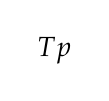
\begin{tikzpicture}[sibling distance=3em, level distance=3em]
  \node {$Tp$};
\end{tikzpicture} &
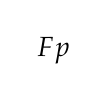
\begin{tikzpicture}[sibling distance=3em, level distance=3em]
  \node {$Fp$};
\end{tikzpicture} &
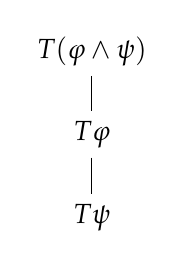
\begin{tikzpicture}[sibling distance=3em, level distance=3em]
  \node {$T (\varphi \land \psi)$}
    child { node {$T \varphi$} 
      child {node {$T \psi$}}};
\end{tikzpicture} &
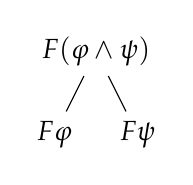
\begin{tikzpicture}[sibling distance=3em, level distance=3em]
  \node {$F (\varphi \land \psi)$}
    child { node {$F \varphi$} }
    child { node {$F \psi$}};
\end{tikzpicture} &
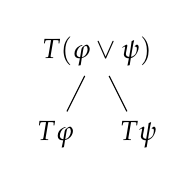
\begin{tikzpicture}[sibling distance=3em, level distance=3em]
  \node {$T (\varphi \lor \psi)$}
    child { node {$T \varphi$} }
    child { node {$T \psi$}};
\end{tikzpicture} &
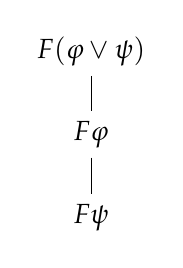
\begin{tikzpicture}[sibling distance=3em, level distance=3em]
  \node {$F (\varphi \lor \psi)$}
    child { node {$F \varphi$} 
      child {node {$F \psi$}}};
\end{tikzpicture} \\
\hline
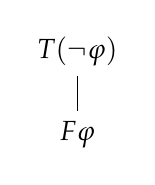
\begin{tikzpicture}[sibling distance=3em, level distance=3em]
  \node {$T (\neg \varphi)$}
    child { node {$F \varphi$} };
\end{tikzpicture} &
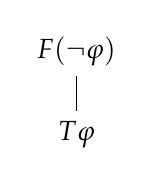
\begin{tikzpicture}[sibling distance=3em, level distance=3em]
  \node {$F (\neg \varphi)$}
    child { node {$T \varphi$} };
\end{tikzpicture} &
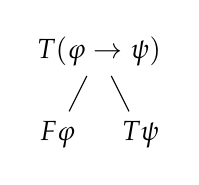
\begin{tikzpicture}[sibling distance=3em, level distance=3em]
  \node {$T (\varphi \to \psi)$}
    child { node {$F \varphi$} }
    child { node {$T \psi$}};
\end{tikzpicture} &
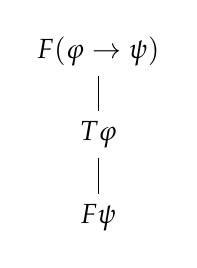
\begin{tikzpicture}[sibling distance=4em, level distance=3em]
  \node {$F (\varphi \to \psi)$}
    child { node {$T \varphi$} 
      child {node {$F \psi$}}};
\end{tikzpicture} &
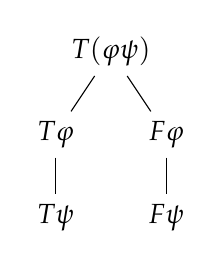
\begin{tikzpicture}[sibling distance=4em, level distance=3em]
  \node {$T (\varphi \lequiv \psi)$}
    child { node {$T \varphi$} 
    	child {node {$T \psi$}}}
    child { node {$F \varphi$} 
    	child {node {$F \psi$}}};
\end{tikzpicture} &
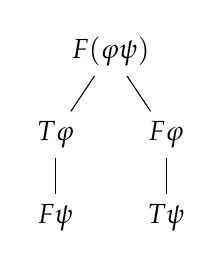
\begin{tikzpicture}[sibling distance=4em, level distance=3em]
  \node {$F (\varphi \lequiv \psi)$}
    child { node {$T \varphi$} 
    	child {node {$F \psi$}}}
    child { node {$F \varphi$} 
    	child {node {$T \psi$}}};
\end{tikzpicture} \\
\hline
\end{tabular}
\end{minipage}
\caption{The atomic tableaux}
\label{fig:prop_tableaux}
\end{figure*}

\informal{The labels in each of the tableaux show, whether a formula $\varphi$ should be true ($T \varphi$) or false ($F \varphi$). The tableaux themselves then ``re-write'' the requirement in their root into more simple requirements. For example, the atomic tableau for $T(\varphi \to \psi)$ expresses that a formula $(\varphi \to \psi)$ is true (T), if $\varphi$ is false ($F \varphi$) or $\psi$ is true $T \psi$. The ``or'' is expressed by the two sons. On the other hand, the atomic tableau for $F(\varphi \to \psi)$ says, that $\varphi \to \psi$ is false, if $\varphi$ is true and $\psi$ is false. The ``and'' is presented by the fact, that both these facts are on a single branch.

While the atomic tableaux are based on the semantics of propositional logic, the tableau method itself is purely syntactic -- it only says, how to manipulate tableaux in order to obtain the proof of a formula.}

Using the atomic tableaux, we can define the tableau in general.

\begin{definition}
A \emph{finite tableau} is a binary tree labeled with entries defined inductively as
\begin{enumerate}
	\item every atomic tableau is a finite tableau,
  \item if $P$ is an entry on a branch $V$ in a finite tableau $\tau$ and $\tau'$ is obtained by adjoining the atomic tableau for $P$ at the end of branch $V$, then $\tau'$ is also a finite tableau,
  \item every finite tableau is formed by finite number of steps above.
\end{enumerate}

A \emph{tableau} $\tau$ is a (potentially infinite) sequence $\tau_0, \tau_1, \dots, \tau_n, \dots$  of finite tableaux such that $\tau_{n+1}$ is formed from $\tau_n$ by an application of step 2 above, formally, $\tau = \bigcup \tau_n$.
\end{definition}

An example of a tableau is shown bellow. In propositional logic, we do not need to repeat the entries that we expand, therefore, we will generally use only the version on the right, where these repeated entries are removed.\sidenote{In predicate logic, some of the repeated entries need to be included in the tableau again.}

\begin{figure}[ht]
\begin{minipage}{0.5\textwidth}
\centering
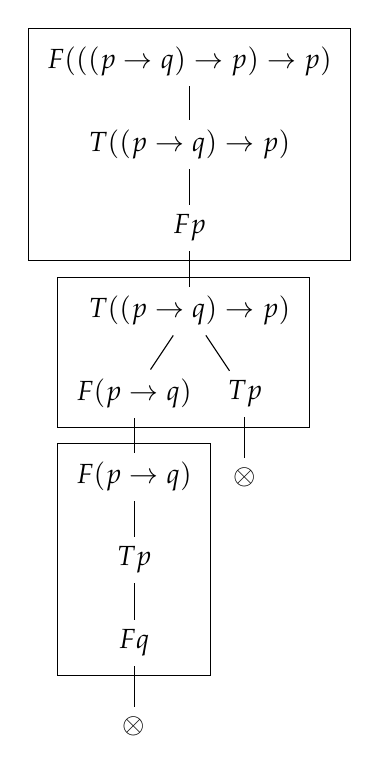
\begin{tikzpicture}[sibling distance=4em, level distance=3em]
  \node(n) {$F(((p \to q) \to p) \to p)$}
    child { node {$T ((p \to q) \to p)$} 
    	child { node {$F p$} 
    		child {node {$T ((p \to q) \to p)$}
    			child {node {$F(p \to q)$}
    				child {node {$F(p \to q)$}
	    				child {node {$Tp$}
	    					child {node {$Fq$}
	    						child {node {$\otimes$}}
	    					}
	    				}
	    			}
    			}
    			child {node {$Tp$}
    				child {node {$\otimes$}}
    			}
    		}
    	}
    };
  \node[fit=(n)(n-1-1), draw] {};
  \node[fit=(n-1-1-1)(n-1-1-1-1), draw] {};
  \node[fit=(n-1-1-1-1-1)(n-1-1-1-1-1-1-1), draw] {};
\end{tikzpicture}
\end{minipage}
\begin{minipage}{0.5\textwidth}
\centering
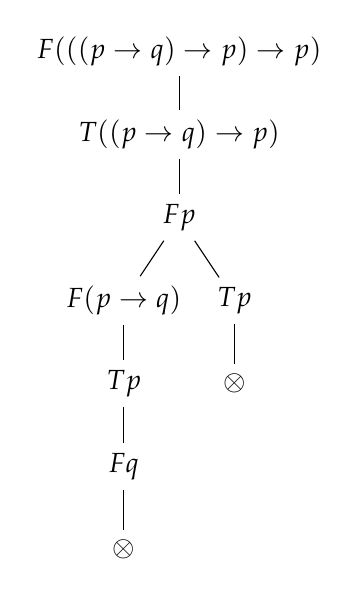
\begin{tikzpicture}[sibling distance=4em, level distance=3em]
  \node(n) {$F(((p \to q) \to p) \to p)$}
    child { node {$T ((p \to q) \to p)$} 
    	child { node {$F p$} 
  			child {node {$F(p \to q)$}
  				child {node {$Tp$}
  					child {node {$Fq$}
  						child {node {$\otimes$}}
  					}
  				}
  			}
  			child {node {$Tp$}
  				child {node {$\otimes$}}
  			}
    	}
    };
\end{tikzpicture}
\end{minipage}
\caption{Example tableau. The rectangles on the left show the atomic tableaux used. The version on the right removes the repeated entries. The symbol $\otimes$ denotes a contradictory branch.}
\label{fig:tableau_notation_proof}
\end{figure}

The definition above does not specify, how to choose the entry $P$ on branch $V$ for expansion. Later, we define the systematic tableau, where this is specified.

Before we can define the formal notion of proof using the tableau method, we first need to discuss some of the terms related to tableaux. For an entry $P$ on a branch $V$ in a tableau $\tau$, we say that \emph{$P$ is reduced on $V$} if it occurs on $V$ as a root of an atomic tableau. A \emph{branch $V$ is contradictory} if it contains entries $T \varphi$ and $F \varphi$ for some proposition $\varphi$, otherwise it is noncontradictory. A \emph{branch $V$ is finished}, if it is contradictory, or every entry on $V$ is reduced on $V$, and finally, a \emph{tableau $\tau$ is finished} if every branch in $\tau$ is finished and $\tau$ is contradictory, if every branch in $\tau$ is contradictory.

A \emph{tableau proof of $\varphi$} is a contradictory tableau with the root entry $F \varphi$. A formula \emph{$\varphi$ is tableau provable} ($\vdash \varphi$) if it has tableau proof. On the other hand, a \emph{refutation of $\varphi$ by tableau} is a contradictory tableau with the root entry $T \varphi$, and \emph{$\varphi$ is tableau refutable} it it has a tableau refutation, in this case we write $\vdash \neg \varphi$.

\informal{Why does a tableau proof of $\varphi$ start with $F \varphi$? Tableaux in fact represent systematic searches for assignments that fulfill the condition expressed by the entry in the root. Therefore, if we cannot find a truth assignment in which $\varphi$ is false (the tableau for $F \varphi$ is contradictory), then $\varphi$ must be true in all assignments, and therefore valid. The formal proof of the soundness and completeness of the tableau methods will be discussed shortly.}

\begin{figure}
\centering
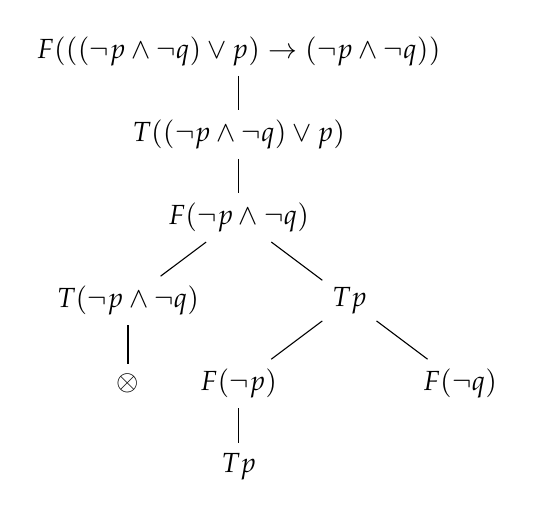
\begin{tikzpicture}[sibling distance=8em, level distance=3em]
  \node {$F(((\neg p \land \neg q) \lor p) \to (\neg p \land \neg q))$}
    child { node {$T ((\neg p \land \neg q) \lor p)$} 
    	child { node {$F (\neg p \land \neg q)$} 
    		child {node {$T (\neg p \land \neg q)$}
    			child {node {$\otimes$}}}
    		child {node {$T p$}
    			child {node {$F(\neg p)$}
    				child {node {$T p$}}}
    			child {node {$F(\neg q)$}}
    			}}
    	};
\end{tikzpicture}
\caption{Example tableau. Both left and middle branches are finished. The left one is also contradictory, while the middle one is noncontradictory. The right branch is not finished.}
\label{fig:tableau_example}
\end{figure}

Figure~\ref{fig:tableau_example} shows a tableau with the root entry $F(((\neg p \land \neg q) \lor p) \to (\neg p \land \neg q))$. The tableau has three branches, the leftmost one is contradictory, as it contains both $F (\neg p \land \neg q)$ and $T (\neg p \land \neg q)$, the middle one is finished and noncontradictory, as every entry on that branch is expanded on it, and the rightmost one is unfinished, as the entry $F (\neg q)$ is not expanded on that branch.

On the other hand, the tableau in Figure~\ref{fig:tableau_notation_proof} is a tableau proof of the proposition $(((p \to q) \to p) \to p)$, as it starts with the entry $F(((p \to q) \to p) \to p)$ and all its branches are contradictory.

We often need to work with theories, and also prove propositions in a theory. Therefore, the notion of tableau needs to be generalized to the notion of tableau from a theory. Theories provide axioms, these are assumed to be true, and therefore the tableau from a theory $T$ can additionally contain entries of the from $T \varphi$ for an axiom $\varphi \in T$. More formally, a \emph{finite tableau from a theory $T$} is a generalized tableau with an additional rule -- if $V$ is a branch of finite tableau (from $T$) and $\varphi \in T$, then by adjoining $T \varphi$ at the end of $V$ we obtain a finite tableau from $T$. The rest of the definitions related to tableaux can be generalized in the same way. \emph{A tableau from $T$} is a sequence $\tau_0, \tau_1, \dots, \tau_n, \dots$ of finite tableaux from $T$ such that $\tau_{n+1}$ is formed from $\tau_n$ applying the rule 2 (from the definition of tableaux), or the additional rule above, formally $\tau = \bigcup \tau_n$. A \emph{tableau proof of $\varphi$ from $T$} is a contradictory tableau from $T$ with $F \varphi$ in the root. $T \vdash \varphi$ denotes that $\varphi$ is tableau provable from $T$. A \emph{refutation of $\varphi$ by a tableau from $T$} is a contradictory tableau from $T$ with $T \varphi$ in the root. A branch $V$ of a tableau from $T$ is finished, if it is contradictory, or every entry on $V$ is already reduced on $V$ and, additionally, $V$ contains $T \varphi$ for each $\varphi \in T$.

While the current definition of tableaux is enough for proving propositions in theories. Here, we provide a stricter definition of so called systematic tableau. We will see later, that a systematic tableau is always finished and, in case the tableau is a proof of a proposition, it is also finite. The definition prescribes the precise order of steps to use while constructing tableaux from theories -- it specifies which entry in the tableau should be expanded next and also which axiom from the theory should be added next.

\begin{definition}
Let $R$ be an entry and $T = \{\varphi_0, \varphi_1, \dots\}$ a theory. Then the \emph{systematic tableau} $\tau$ from $T$ for the entry $R$ is the result of the following construction, i.e. $\tau = \bigcup \tau_n$
\begin{enumerate}
	\item $t_0$ is the atomic tableau for $R$, then proceed with the following steps until possible
	\item Let $P$ be the leftmost entry in the smallest possible level of the tableau $\tau_n$, such that $P$ is not reduced on some noncontradictory branch through $P$.
	\item Let $\tau'_n$ be the tableau obtained from $\tau_n$ by adjoining the atomic tableau for $P$ to every noncontradictory branch through $P$ ($\tau'_n = \tau_n$ if no such $P$ exists).
	\item Let $\tau_{n+1}$ be the tableau obtained from $\tau'_n$ by adjoining $T \varphi_n$ to every noncontradictory branch that does not contain $T \varphi_n$ (if $\varphi_n$ does not exist, $\tau_{n+1}=\tau'_n$).
\end{enumerate}
\end{definition}

The first thing to notice is that every systematic tableau is finished. Assume we have a tableau $\tau = \bigcup \tau_n$. If there is a noncontradictory branch in $\tau$, the prefix of this branch is noncontradictory in each $\tau_n$. Therefore, the branch must contain $T \varphi_n$ for each $\varphi_n$ in $T$. Let us now assume, there is an entry $R$, such that $R$ is not reduced on a branch. However, there are only finitely many levels above $R$ in $\tau$ and therefore only finitely many entries above $R$, thus $R$ will be eventually selected in step 2 and reduced in step 3, which is a contradiction with $R$ not being reduced. So, every noncontradictory branch in the tableau is finished (it contains $T \varphi_n$ for each $\varphi_n \in T$, and every entry on the branch is reduced).

Interestingly, if tableau is used as a proof, it is not only finished, it is also finite. More specifically -- for every contradictory tableau $\tau = \bigcup t_n$, there is some $n$ such that $\tau_n$ is contradictory finite tableau. Why? Let $S$ be the set of nodes in $\tau$ that have no pair of contradictory entries $T \varphi$, $F \varphi$ amongst their predecessors. We can imagine this set as a ``top part'' of the tableau -- the root is definitely in this set. If there is a node in the set, all of its predecessors are also there. Such a set $S$ must be finite, because otherwise, by König's lemma, the subtree of $\tau$ induced by the set $S$ would have an infinite branch (it is a finitely branching infinite tree), and therefore the tableau $\tau$ would not be contradictory. Now, since $S$ is finite, all of the nodes in $S$ belong to levels up to $m$ for some $m$. Thus every node in level $m+1$ has a pair of contradictory entries among its predecessors. We can now choose $n$ such that the top $m+1$ levels of $\tau$ are a subtree of $\tau_n$. Every branch in $\tau_n$ now contains a pair of contradictory entries and is thus contradictory.

In the construction of systematic tableaux, we extend only noncontradictory branches, therefore if a systematic tableau (from a theory) is a proof, it is finite (remember that a proof is a contradictory tableau with $F \varphi$ in its root). This is an important results, it shows that if a formula has a proof, we have an algorithm (the construction of systematic tableau) that can find the proof in finite amount of time. It also shows that any proof from a theory depends only on a finite number of axioms from the theory. 

\section{Soundness and Completeness}

Now, we want to show the soundness and completeness of the tableau method. We start with the soundness and show, that if a formula has a tableau proof from a theory, the formula is also valid in the theory. However, before we get to the proof, we need a definition and a lemma. We say that an \emph{entry $P$ agrees with an assignment $v$}, if $P$ is $T \varphi$ and $\bar{v}(\varphi) = 1$, or if $P$ is $F \varphi$ and $\bar{v}(\varphi) = 0$. A \emph{branch $V$ agrees with $v$} if every entry on $V$ agrees with $v$. 

\begin{lemma}
Let $v$ be a model of a theory $T$ that agrees with the root entry of a tableau $\tau = \bigcup \tau_n$. Than $\tau$ contains a branch that agrees with $v$.
\end{lemma}
\begin{proof}
We will find a sequence $V_0, V_1, \dots$ for every $n$, such that $V_n$ is a branch in $\tau_n$, $V_n \subseteq V_{n+1}$ and $V_n$ agrees with $n$. We start by verifying the lemma for all atomic tableaux, thus verifying the base of the induction. For example, if we have $v(p) = 1, v(q) = 0$ and the atomic tableau with root entry $T(p \lor q)$, then $v$ agrees with the root entry, and the branch of the tableau containing $Tp$ also agrees with $v$. We can check the other atomic tableaux similarly. Now, if $\tau_{n+1}$ is obtained from $\tau_n$ without extending $V_n$, we take $V_{n+1} = V_n$. If $\tau_{n+1}$ is obtained from $\tau_n$ by adjoining $T \varphi$ to $V_n$ for some $\varphi \in T$, let $V_{n+1}$ be this branch, $v$ agrees with $V_{n+1}$ as $v$ is a model of $T$ (and therefore all axioms of $T$ are true in $v$). Finally, if $\tau_{n+1}$ is obtained from $\tau_n$ by adjoining the atomic tableau for some entry $P$ on $V_n$ to the end of $V_n$, we can extend $V_n$ to $V_{n+1}$ as required as $P$ agrees with $v$ and all atomic tableaux are verified (for example, if $P = T(p\lor q)$, and $v$ is as in example on atomic tableaux above, we obtain $V_{n+1}$ by adding $T(p \lor q)$ and $Tp$ to the end of $V_n$).
\end{proof}

Using the lemma, we can now easily proof the soundness of the tableau method in propositional logic.

\begin{theorem}[Soundness of tableau method in propositional logic]
For every theory $T$ and proposition $\varphi$, if $\varphi$ is tableau provable from $T$, then $\varphi$ is valid in $T$, i.e. $T \vdash \varphi \Rightarrow T \vDash \varphi$.
\end{theorem}
\begin{proof}
If $\varphi$ is tableau provable from $T$, there is a contradictory tableau $\tau$ from $T$ with the root entry $F \varphi$. Suppose $\varphi$ is not valid in $T$. In such a case, there is a model $v$ of the theory $T$ in which $\varphi$ is false. Therefore, the root entry of the proof ($F \varphi$) agrees with $v$ and by the previous lemma, there is a branch in $\tau$ that agrees with $v$. However, that leads to contradiction as $\tau$ is the proof of $\varphi$ from $T$, and therefore every branch of $\tau$ is contradictory and cannot agree with $v$.
\end{proof}

The soundness theorem says that whenever we have a tableau proof of a formula in a theory, the formula is valid. However, can we also prove any valid formula using the tableau method? We indeed can, as the completeness theorem states. Again, before we get to the proof of the completeness theorem, we prove a helper lemma, that formally shows that a noncontradictory branch in a finished tableau provides a counterexample.

\begin{lemma}
Let $V$ be a noncontradictory branch of a finished tableau $\tau$. Then $V$ agrees with the following assignment $v$: $$v(p) = \twopartdefotherwise{1}{Tp \text{ occurs on } V}{0}$$
\end{lemma}
\begin{proof}
We prove the lemma by induction on the structure of formulas in entries on $V$.
\begin{itemize}
 \item For entry $T p$ on $V$, where $p$ is a propositional variable, we have $\bar{v}(p)= 1$ by definition.
 \item For entry $F p$ on $V$, the entry $T p$ is not on $V$ as $V$ is noncontradictory, and thus we have $\bar{v}(p) = 0$ by definition.
 \item For entry $T (\varphi \land \psi)$, we have both $T \varphi$ and $T \psi$ on $V$ as $\tau$ is finished, and by induction, we know $\bar{v}(\varphi)=\bar{v}(\psi)=1$, therefore $\bar{v}(\varphi \land \psi)=1$ and $v$ agrees with $T (\varphi \land \psi)$.
 \item For entry $F (\varphi \land \psi)$, we have $F \varphi$ or $F \psi$ on $V$ as $\tau$ is finished, therefore we have $\bar{v}(\varphi) = 0$, or $\bar{v}(\psi) = 0$, which leads to $\bar{v}(\varphi \land \psi) = 0$ and thus $v$ agrees with $F (\varphi \land \psi)$.
\end{itemize}

The lemma can be proven for the other possible types of entries (with $\lor, \to, \lequiv, \neg$) similarly to the last two steps for entries with $\land$.
\end{proof}

Using this lemma, it is simple to prove the completeness theorem.

\begin{theorem}
For every theory $T$ and proposition $\varphi$, if $\varphi$ is valid in $T$, then $\varphi$ is tableau provable from $T$, i.e. $T \vDash \varphi \Rightarrow T \vdash \varphi$.
\end{theorem}
\begin{proof}
We will show that an arbitrary finished tableau $\tau$ from theory $T$ with root entry $F \varphi$ is contradictory, if $\varphi$ is valid in $T$.

Assume (for contradiction), there is noncontradictory branch $V$ in $\tau$. The previous lemma provides an assignment $v$, such that $V$ agrees with $v$, therefore also the root entry $F \varphi$ agrees with $v$ and thus $\bar{v}(\varphi) = 0$. Since $V$ is finished, it contains $T \psi$ for every $\psi \in T$, but that means that $v$ is a model of $T$ ($V$ agrees with $v$, therefore $\bar{v}(\psi) = 1$ for all $\psi \in T$). However, this is contradiction with the assumption that $\varphi$ is valid in $T$, therefore every branch in $\tau$ is contradictory and $\tau$ is a proof of $\varphi$ from $T$. 
\end{proof}

We can now introduce syntactic definition of the semantic terms defined earlier and discuss the relation between the syntactic and semantic notions. First of all, we define the \emph{set of proposition provable from $T$} $$\Thm^\Prop(T) = \{\varphi | \varphi \in \VF_\Prop, T \vdash \varphi\}\,.$$ We say that a theory \emph{$T$ is inconsistent}, if $T \vdash \bot$, otherwise \emph{$T$ is consistent}. A theory \emph{$T$ is complete}, if it is consistent and every proposition is provable or refutable from $T$, i.e. if $T \vdash \neg \varphi$ or $T \vdash \varphi$ for every $\varphi \in \VF_\Prop$. A theory $T$ over $\Prop$ is \emph{an extension} of $T'$ over $\Prop'$, if $\Prop' \subseteq \Prop$ and $\Thm^{\Prop'}(T') \subseteq \Thm^{\Prop}(T)$, the extension is \emph{simple}, if $\Prop = \Prop'$, and it is \emph{conservative} if $\Thm^{\Prop'}(T') = \Thm^{\Prop}(T) \cap \VF_{\Prop'}$. Two \emph{theories $T$ and $T'$ are equivalent}, if $T$ is an extension of $T'$ and vice versa.

There are strong relations between the syntactic terms introduced above and the semantic terms introduced in the previous chapter. Most of these are corollaries of the soundness and completeness of tableau method. For each theory $T$ and propositions $\varphi, \psi$ over $\Prop$ 
\begin{enumerate}
	\item $T \vdash \varphi$ if and only if $T \vDash \varphi\,,$
	\item $\Thm^\Prop(T) = \theta^\Prop(T)\,,$
	\item $T$ is inconsistent if and only if $T$ is unsatisfiable, i.e. it has no model,
	\item $T$ is complete if and only if $T$ is semantically complete, i.e. it has a single model,
	\item (deduction theorem) $T \cup \{\varphi\} \vdash \psi$ if and only if $T \vdash \varphi \to \psi\,.$
\end{enumerate}

Another important corollary of the theorems is the compactness theorem.

\begin{theorem}
A theory $T$ has a model if and only if every finite subset of $T$ has a model.
\end{theorem}
\begin{proof}
The implication to right (if a theory has a model, every finite subset has a model) is trivial. In order to prove the other implication, we first realize that if $T$ has no model, it is inconsistent, thus $T \vdash \bot$ and $\bot$ is provable by a systematic tableau $\tau$ from $T$. The tableau is finite, therefore $\tau$ is also provable from a finite subset of $T' \subseteq T$ ($T'$ contains the axioms from $T$ that were used in the proof), $T'$ is inconsistent and, therefore, has no model.
\end{proof}

While the compactness theorem is interesting itself, it is also a very strong theorem that can be used to prove other theorems in different parts of mathematics. Consider for example the theorem on infinite $k$-colorable graphs\sidenote{A graph is $k$-colorable if there is a function $c: V \to k$, such that $c(u)\neq c(v)$ for every edge $\{u,v\}\in E$.}: a countably infinite graph $G = (V, E)$ is $k$-colorable if and only if each finite subgraph of $G$ is $k$-colorable. Again, if the infinite graph is colorable, every finite subgraph is obviously also colorable. The other implication is more interesting. Consider a set of propositional variables $\Prop = \{p_{u,i} | u \in V, i \in k\}$, where $p_{u,i}$ means that vertex $u$ has color $i$. We can create a theory $T$ with axioms $p_{u,0} \lor p_{u,1} \lor \dots \lor p_{u,k-1}$ for each $u \in V$ (every vertex has a color), $\neg(p_{u,i} \land p_{u,j})$ for every $u \in V, i < j < k$ (every vertex has only one color), and $\neg(p_{u,i} \land p_{v,i})$ for each $\{u,v\}\in E, i < k$ (two vertices connected with an edge do not have the same color). Obviously, $G$ is colorable if and only if $T$ has a model. We only need to show, that every finite $T' \subseteq T$ has a model (and use the compactness theorem). Let $G'$ be a subgraph of $G$ induced by  vertices $u$ such that $p_{u,i}$ appears in $T'$ for some $i$. By assumption, $G'$ is $k$-colorable, and therefore $T'$ has a model.

\section{Hilbert systems}

A (more traditional) alternative to the tableau method is the Hilbert calculus. In this proof system, formulas are defined using only implication ($\to$) and negation ($\neg$), and all other logical connectives are defined using these two (we already know, that the set $\{\to, \neg\}$ is adequate, so this can be done). The Hilbert proof system then defines the following set of schemas of axioms (for two proposition $\varphi, \psi \in \VF_\Prop$):
\begin{enumerate}
\item $\varphi \to (\psi \to \varphi)$
\item $(\varphi \to (\psi \to \chi)) \to ((\varphi \to \psi) \to (\varphi \to \chi))$
\item $(\neg \varphi \to \neg \psi) \to (\psi \to \varphi)$
\end{enumerate}
Apart from the axioms, there is also a single inference rule: \emph{modus ponens}, which can be expressed as $$\frac{\varphi, \varphi \to \psi}{\psi}\,.$$That means that if $\varphi$ and $\varphi \to \psi$ are true we can infer that also $\psi$ is true.

A proof of formula $\varphi$ from a theory $T$ in the Hilbert-style is defined as a finite sequence of formulas $\varphi_0, \varphi_1, \dots \varphi_n = \varphi$ such that for every $i \leq n$, $\varphi_i$ is a logical axiom, or an axiom from the theory ($\varphi_n \in T$), or $\varphi_i$ is inferred from $\varphi_j$ and $\varphi_k$ ($j,k < i$) using the modus ponens rule. As with tableau method, a formula $\varphi$ is provable from $T$ ($T \vdash_H \varphi$), if it has a proof.

For example, we can show, that $\varphi \to \psi$ is provable from $T = \{\neg \varphi\}$ for every $\psi$.

\begin{enumerate}
\item $\neg \varphi$
\item $\neg \varphi \to (\neg \psi \to \neg \varphi)$
\item $\neg \psi \to \neg \varphi$
\item $(\neg \psi \to \neg \varphi) \to (\varphi \to \psi)$
\item $\varphi \to \psi$
\end{enumerate}

The first two steps are axiom of a theory and logical axiom (the schema number 2). The third formula is obtained from the previous two by modus ponens, the fourth one is again an axiom (by schema number 3), and the last one is obtained from formulas number 3 and 4 using modus ponens.

It is easy to prove the soundness of the Hilbert calculus ($T \vdash_H \varphi \Rightarrow T \vDash \varphi$). Logical axioms are tautologies, and axioms from $T$ hold in all models of $T$, therefore the soundness holds for axioms of any kind, and the modus ponens rule is sound (as can be easily checked using the truth tables of $\varphi$, $\varphi \to \psi$, and $\psi$). Thus, the soundness is proved. The Hilbert calculus is also complete, but we will not show the proof here.

\section{Resolution method}

The resolution method is the base of many automated systems -- SAT solvers, automated deduction or verification systems and Prolog\sidenote{Prolog is a programming language based on the specification of programs as sets of Horn formulas.} interpreters. The method assumes the input formulas are given in CNF and it works with a set representation of the formulas (a CNF formula is represented as a set of sets of literals). The method has no explicit axioms, but some of the axioms are implicitly included. It uses a single inferences rule (the resolution rule). Similarly to the tableau method, the resolution method is also a refutation procedure, i.e. it tries to show that a given formula or theory is unsatisfiable. There are several variants of the resolution method that gives more specific rules on when the resolution rule can be applied (e.g. the LI resolution, or the SLD resolution).

Before we describe the resolution method formally, we must define the set representation of CNF formulas. Similarly to our discussion on CNF formulas, a literal is either a propositional variable or its negation. The complementary literal to $l$ is still denoted as $\bar{l}$. A \emph{clause} $C$ is a finite set of literals, and an \emph{empty clause}, denoted as $\square\,,$ is never satisfied. A \emph{formula $S$} is then a (possibly infinite) set of clauses. An empty formula $\emptyset$ is always satisfied. Infinite formulas represent infinite theories. A \emph{(partial) assignment $\mathcal{V}$} is a consistent set of literals (i.e. the set does not contain a complementary pair of literals). An assignment is \emph{total}, if it contains a positive or negative literal for each propositional variable. An assignment $\mathcal{V}$ satisfies a formula $S$ (denoted as $\mathcal{V} \vDash S$), if $C \cap \mathcal{V} \neq \emptyset$ for each clause $C \in S$.

For example, the CNF-formula $((\neg p \lor q) \land (\neg p \lor \neg q \lor r) \land (\neg r \lor \neg s) \land s)$ is represented as $S = \{\{\neg p, q\}, \{\neg p, \neg q, r\}, \{\neg r, \neg s\}, \{s\}\}$ and $\mathcal{V} = \{s, \neg r, \neg p\}$ is a satisfying assignment for $S$.

\informal{While the definitions above are different from those we used previously, they are in fact equivalent. The only reason why they are worded differently is the set representation of the CNF formulas. We know that a formula in CNF is a conjunction of clauses, therefore, we can only represent them as a set of clauses. A clause is a disjunction of literals, and therefore it is again natural to represent each clause as a set of literals. The definition of assignment may seem strange, but the set of literals only says which literals are true and which are false.}

There is only one inference rule in resolution -- the resolution rule: let $C_1$ and $C_2$ are clauses such that $l \in C_1$ and $\bar{l} \in C_2$, then infer a clause $C$ (called a resolvent) such that $C = (C_1 \setminus \{l\}) \cup (C_2 \setminus \{\bar{l}\})$. The resolution rule is a special case of the cut rule: $$\frac{\varphi \lor \psi \qquad \neg \varphi \lor \chi}{\psi \lor \chi}\,,$$ for any formulas $\varphi, \psi, \chi$. 

It is easy to realize that the resolution rule is sound, i.e. if $\mathcal{V} \vDash C_1$ and $\mathcal{V} \vDash C_2$, then $\mathcal{V} \vDash C$ -- the assignment $\mathcal{V}$ cannot contain a pair of complementary literals (by definition), therefore at least one of the intersections $\mathcal{V} \cap (C_1 \setminus \{l\})$ or $\mathcal{V} \cap (C_2 \setminus \{\bar{l}\})$ must be non-empty, therefore $\mathcal{V} \cap C$ is also non-empty.

A \emph{resolution proof (deduction) of a clause $C$ from formula $S$} is a finite sequence of clauses $C_0, C_1, \dots, C_n = C$ such that for each $i \leq n$, $C_i \in S$, or $C_i$ is a resolvent of some previous clauses. As usual, a \emph{clause $C$ is provable from formula $S$} ($S \vdash_R C$), if it has a resolution proof from $S$. We already mentioned that resolution is used as a refutation procedure. A \emph{resolution refutation of formula $S$} is a resolution proof $S \vdash_R \square$, and a \emph{formula is resolution refutable}, if there is such a proof.

Let us now show, that resolution is also a sound and complete method. The soundness is simple, and follows from the soundness of the resolution rule.

\begin{theorem}[Soundness of resolution]
If a formula $S$ is resolution refutable, it is unsatisfiable.
\end{theorem}
\begin{proof}
Let $S \vdash_R \square$ and assume (for contradiction) there is an assignment $\mathcal{V}$ such that $\mathcal{V} \vDash S$. Because the resolution rule is sound, also $\mathcal{V} \vDash \square$, but that is not possible ($\square$ is never satisfied).
\end{proof}

The proof of completeness is a bit more involved. To this end, we first define resolution trees, which in fact show, how we obtained a proof of a clause. A \emph{resolution tree} of clause $C$ from formula $S$ is a finite binary tree with nodes labeled by clauses such that the root is labeled by $C$, the leaves are labeled by clauses from $S$, and every inner node is labeled by the resolvent of its sons. Obviously, there is a resolution tree for $C$ from $S$ if and only if $S \vdash_R C$.

Another important notion is the \emph{resolution closure} of a formula $S$, denoted as $\mathcal{R}(S)$ and defined as the smallest set containing all clauses of $S$ and closed under the resolution rule, i.e. if $C_1, C_2 \in \mathcal{R}(S)$ and $C$ is the resolvent of $C_1$ and $C_2$, then also $C \in \mathcal{R}(S)$. Obviously, $C \in \mathcal{R}(S)$ if and only if $S \vdash_R C$, and all the notions on resolution proofs can be also defined using the resolution trees and closures.

As a simple example of the resolution method, we can show that formula $S = \{\{p, r\}, \{q, \neg r\}, \{\neg q\}, \{\neg p, t\}, \{\neg s\}, \{s, \neg t\}\}$ is unsatisfiable as $S \vdash_R \square$.

\begin{figure}
\centering
\begin{tikzpicture}[level 1/.style={sibling distance=15em}, 
                    level 2/.style={sibling distance=8em}, 
                    level distance=4em]
  \node {$\square$}
    child { node {$\{p\}$} 
      child {node {$\{p, q\}$} 
        child {node {$\{p, r\}$}}
        child {node {$\{q, \neg r\}$}}
      }
      child {node {$\{\neg q\}$}} 
    }
    child { node {$\{\neg p\}$}
      child { node {$\{\neg p, s\}$}
        child { node {$\{\neg p, t\}$}}
        child { node {$\{s, \neg t\}$}}
      }
      child { node {$\{\neg s\}$}}  
    };
\end{tikzpicture}
\caption{The resolution proof of $S \vdash_R \square$.}
\end{figure}

We can also compute the resolution closure 
\begin{align*}
\mathcal{R}(S) =  \{ & \{p, r\}, \{q, \neg r\}, \{\neg q\}, \{\neg p, t\}, \{\neg s\}, \{s, \neg t\}, \{p, q\}, \\ 
& \{\neg r\}, \{r,t\}, \{q,t\}, \{\neg t\}, \{\neg p, s\}, \{r,s\}, \{t\}, \{q\}, \\ 
& \{q,s\}, \square, \{\neg p\}, \{p\}, \{r\}, \{s\}\}\,,
\end{align*}
and as $\square \in \mathcal{R}(S)$, we also know that $S$ in unsatisfiable.

In the proof of completeness, we will use the notion of reduction by substitution. Let $S$ be a formula and $l$ a literal, we define $$S^l = \{C \setminus \{\bar{l}\}| l \notin C \in S\}\,.$$ The new formula $S^l$ is in fact equivalent to a formula, where the literal $l$ was assigned a true value ($\top$) and $\bar{l}$ was assigned false value ($\bot$). In such a case, any clause containing $l$ can be removed (as it is satisfied), and $\bar{l}$ is removed from all other clauses. The formula $S^l$ does not contain any of the literals $l$ and $\bar{l}$, and if $S$ contained a clause $\{\bar{l}\}$, then $S^l$ contains $\square$.

In the proof of completeness of the resolution method, we will need the following lemma.

\begin{lemma}
A formula $S$ is satisfiable if and only if $S^l$ or $S^{\bar{l}}$ is satisfiable.
\end{lemma}
\begin{proof}
Let $\mathcal{V} \vDash S$ and (without loss of generality) $\bar{l} \in \mathcal{V}$. Then, $\mathcal{V} \vDash S^l$, as for clauses $C$ such that $l \notin C \in S$, $\mathcal{V} \vDash C \setminus \{\bar{l}\}$, as $\mathcal{V}$ does not contain $\{\bar{l}\}$ and it is satisfying for each clause $C \in S$.

On the other hand, assume (without loss of generality) $\mathcal{V} \vDash S^l$ for some $\mathcal{V}$. Since neither $l$ nor $\bar{l}$ occur in $S^l$, $\mathcal{V}' = (\mathcal{V} \setminus \{\bar{l}) \cup \{l\}\} \vDash S^l$. Then, $\mathcal{V}' \vDash S$, as for $C \in S$, such that $l \in C$, also $l \in \mathcal{V}$ and for $C \in S$ not containing $l$, we have $\mathcal{V}' \vDash (C \setminus \{\bar{l}\}) \in S^l$.
\end{proof}

The reductions of literals can be represented in a binary tree -- so called reduction tree. The root of the tree is the formula $S$ and each node $N$ has two sons -- $N^l$ and $N^{\bar{l}}$. With the reduction tree, formula $S$ is unsatisfiable if and only if every branch contains $\square$.

\begin{figure}
\centering
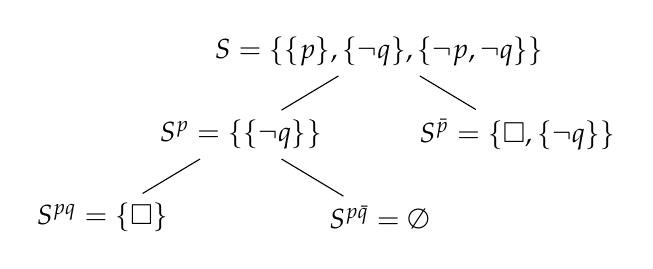
\begin{tikzpicture}[sibling distance=10em, level distance=3em]
  \node {$S = \{\{p\}, \{ \neg q\}, \{\neg p, \neg q\}\}$}
    child { node {$S^p = \{\{\neg q\}\}$} 
      child {node {$S^{pq} = \{\square\}$}}
      child {node {$S^{p\bar{q}} = \emptyset$}} 
    }
    child { node {$S^{\bar{p}} = \{\square, \{\neg q\}\}$}};
\end{tikzpicture}
\caption{An example of a reduction tree.}
\end{figure}

Interestingly, since $S$ can be infinite over countable language, the tree can also be infinite. However, if $S$ is unsatisfiable, according to the compactness theorem, there is a finite $S' \subseteq S$ such that $S'$ is unsatisfiable. Therefore, after the reduction of all literals from $S'$, there will be $\square$ on every branch after finitely many steps.

Finally, we can prove the completeness of the resolution. The theorem bellow shows the completeness for finite formulas, the general version is obtained from that theorem by using the compactness, similarly to the discussion on the reduction trees above.

\begin{theorem}[completeness of resolution]
If a finite $S$ is unsatisfiable, it is resolution refutable, i.e. $S \vdash_R \square$.
\end{theorem}
\begin{proof}
We will prove the theorem by induction on the number of variables in $S$. There is only one unsatisfiable $S$ without variables -- \{$\square$\} and therefore $S \vdash_R \square$ (the proof is the single step $\square$).

Let us now assume, that $S$ is unsatisfiable and contains a literal $l$. Then, by the previous lemma, $S^l$ and $S^{\bar{l}}$ are unsatisfiable. These contain less literals than $S$ and therefore by induction there are resolution trees $T^l$ and $T^{\bar{l}}$ for derivation of $\square$ from $S^l$ and $S^{\bar{l}}$ respectively. Now, if every leaf of $T^l$ is in $S$, then $T^l$ is a resolution tree of $\square$ from $S$ and therefore $S \vdash_R \square$. Otherwise, we can append the literal $l$ to each leaf of $T^l$ which is not in $S$ and to all of its predecessors, thus obtaining the resolution tree for $\{l\}$ from $S$ (if the original leaf was not in $S$, the one with added $l$ will be, as the only difference between $S^l$ and $S$ is the removal of $l$). Similarly, by appending $\{\bar{l}\}$ to leaves in $T^{\bar{l}}$ we obtain resolution tree for $\{\bar{l}\}$ from $S$. Resolving the roots of these trees yields the resolution tree of $\square$ from $S$.
\end{proof}

We already mentioned that resolution is widely used in different automated systems -- SAT solvers, formal verification systems etc. One of the important examples is the Prolog interpreter. Prolog is a programming language, where programs are sets of Horn clauses. The program can then answer queries (goals). As the Prolog programs are limited to Horn formulas, the resolution method can be improved. The Prolog interpreter uses so called SLD resolution which is based on LD resolution and that is in turn based on LI resolution, which is a special case of linear resolution. Therefore, we will now define the linear resolution, show that LI resolution is complete for Horn formulas and finally define the LD and SLD resolution as simple improvements of the LI resolution.

\subsection{Linear resolution}

The general resolution procedure can be further simplified without losing the completeness. We define a linear proof of a clause $C$ from a formula $S$ as a finite sequence of pairs $(C_0, B_0), \dots, (C_n, B_n)$, such that $C_0 \in S$ and for every $i \leq n$, $B_i \in S$ or $B_i = C_j$ for some $j < i$, and $C_{i+1}$ is a resolvent of $C_i$ and $B_i$, where $C_{n+1} = C$. In the linear proof $C_0$ is called the \emph{starting clause}, $C_i$ a \emph{central clause}, and $B_i$ a \emph{side clause}. Again, we say that $C$ is \emph{linearly provable} from $S$ ($S \vdash_L C$), if it has a linear proof from $S$. A linear proof of $\square$ from $S$ is a \emph{linear refutation} of $S$ and $S$ is \emph{linearly refutable} if $S \vdash \square$.

Obviously, every linear proof can be transformed into a general resolution proof and therefore the linear resolution is also sound. Moreover, is is also complete (we omit the proof of completeness here).

%TODO: \add{Example of linear resolution}

\subsection{LI-resolution}

If we deal with Horn formulas, we can use an even more refined resolution procedure called linear input (LI) resolution. A LI-resolution from a formula $S$ is a linear resolution from $S$ where each side clause $B_i$ is from the input formula $S$ (i.e. $B_i$ cannot be a previously resolved central clause). We write $S \vdash_{LI} C$ to denote that $C$ is provable by LI-resolution from $S$.

We already defined Horn formulas while discussing the satisfiability problem. The definition from the resolution point of view is similar, the only difference is that we again use the set representation instead of the general one (and also formulas in this case can be infinite, as there is no distinction between theories and formulas in resolution). So, a \emph{Horn clause} is a finite set of literals containing at most one positive literal. A Horn formula is then a (potentially infinite) set of Horn clauses. A clause \{p\}, where $p$ is a positive literal is called a \emph{fact}, and a clause with exactly one positive literal is called a \emph{rule}. Rules and facts are also called \emph{program clauses}. A non-empty Horn clause without any positive literal is called a \emph{goal}.

We can easily see that if a Horn formula $S$ is unsatisfiable and it does not contain $\square$, it must contain some fact and some goal. Why? If $S$ does not contain any fact, it is satisfied by setting all the propositional variables to 0. if it does not contain any goal, it is satisfied by setting all variables to 1.

The LI-resolution is complete for Horn formulas, as the following theorem says. The proof of the theorem is similar to the proof of completeness of general resolution.

\begin{theorem}[completeness of LI-resolution]
If $T$ is satisfiable Horn formula but $T \cup \{G\}$ is unsatisfiable for some goal $G$, then $\square$ a LI-resolution from $T \cup \{G\}$ with starting clause $G$.
\end{theorem}
\begin{proof}
As in the proof of completeness of general resolution, we use induction on the number of variables, this time in $T$. By the observation above, $T$ must contain a fact $\{p\}$ for some variable $p$ ($T \cup \{G\}$) is unsatisfiable, therefore it must contain a goal and a fact, $G$ is a goal, so the fact must be in $T$). By the lemma we used in the proof of completeness of general resolution, $T' = (T \cup \{G\})^p = T^p \cup \{G^p\}$ is unsatisfiable and $G^p = G \setminus \{\neg p\}$. Now, if $G^p = \square$, we have $G = \{\neg p\}$ and thus $\square$ is a resolvent of $G$ and $\{p\}\in T$. Otherwise, since $T^p$ is satisfiable (by the satisfying assignment for $T$) and has less variables, by induction assumption, there is an LI-resolution of $\square$ form $T'$ starting with $G^p$. If we now append the literal $\neg p$ to all leaves that are not in $T \cup \{G\}$ (and their predecessors), we have an LI-resolution proof of $\{\neg p\}$ from $T$, we can resolve it with $\{p\}$ from $T$ to obtain the LI-resolution proof of $\square$ from $T$.
\end{proof}

\subsection{Resolution in Prolog}

A program in Prolog is a set of program clauses (i.e. rules or facts), an example program is shown bellow (the program contains seven clauses, the numbers indicate line numbers and are not a part of the program):

\begin{verbatim}
1: p:-q,r.                    5: r.
2: p:-s.                      6: s:-t.
3: q.                         7: s.
4: q:-s.
\end{verbatim}

The formulas on lines 3, 5, and 7 are facts, the rest are rules. The symbol \texttt{:-} can be interpreted as an implication from right to left ($\leftarrow$). So, the meaning of the clauses is as given bellow:

\begin{multicols}{2}
\begin{enumerate}
  \item $q \land r \to p$
  \item $s \to p$
  \item $q$
  \item $s \to q$
  \columnbreak
  \item $r$
  \item $t \to s$
  \item $s$
\end{enumerate}
\end{multicols}

In Prolog, we want to know whether a query is a consequence of a given program. A query is a conjuction of goals (positive literals), e.g. $p \land q$. That means, the question is, whether for a program $P$ and query ($q_1 \land \dots \land q_n$), it holds that $P \vDash (q_1 \land \dots \land q_n)$. However, such a question is equivalent to the fact that $P \cup \{\neg q_1, \dots, \neg q_n\}$ is unsatisfiable, which is equivalent to $\square$ having LI-resolution from $P \cup \{G\}$ starting with goal $G = \{\neg q_1, \dots, \neg q_n\}$.

In the Prolog interpreter, the clauses are represented as sequences of literals (as opposed to sets of literals as in LI resolution). Therefore, Prolog uses a slightly different version of LI-resolution called the LD-resolution (linear definite). In LD resolution, the resolvent of a goal $(\neg p_1, \dots, \neg p_{i-1}, \neg p_i, \neg p_{i+1}, \dots, \neg p_n)$ and a rule $(p_i, \neg q_1, \dots, \neg q_m)$ is a new goal $(\neg p_1, \dots, \neg p_{i-1}, \neg q_1, \dots, \neg q_m, \neg p_{i+1}, \dots, \neg p_n)$, i.e. one of the negative literals in the current goal is replaced by the negative literals from the rule. 

The LD resolution does not specify, which of the negative literals in the goal should be resolved next. This would make programming in Prolog hard, therefore it extends the LD resolution with a selection rule $\mathcal{R}$. Typically, the rule is ``select the first literal''. More formally, an SLD-resolution via $\mathcal{R}$ is an LD-resolution in which each step $(C_i, B_i)$ we resolve through $\mathcal{R}(C_i)$.

Obviously, any LI-resolution can be expressed as LD-resolution (just use the sequences of literals instead of the sets of literals), and any LD-resolution can be expressed as an SLD-resolution with the correct selection rule
 (select the literal that was selected in the LD resolution). Therefore, we can see that SLD resolution is complete for Prolog programs.

Further discussion on Prolog is out of the scope of this lecture, so we will omit it here. The important message was to show an application of logic in computer science. Prolog is quite often used in certain areas of artificial intelligence.

\bigskip

This concludes the part of the lecture dedicated to propositional logic. We started with the discussion about the syntax of propositions, explained their semantics and showed some formal proof systems. In the next part of the lecture, we will build on the understanding of concepts from  propositional logic and extend them to predicate logic (more precisely to first order logic).


\part{First-Order Logic}

%!TEX root = main.tex

\chapter{Basic Syntax and Semantics}

We are now ready to discuss the predicate logic, mostly the first-order logic. The language of predicate logic is more expressive than the one of propositional logic and allows us to express complex formulas in a much more concise way. In propositional logic, we often needed to use many variables and created long formulas. In predicate logic, some of these can be written more elegantly, as we can now use functions, relations, and logical quantifiers.

This whole part will follow the structure of the previous one -- we will again start by the basic syntax and semantics of predicate logic, then we will discuss the logical theories and their models, the tableau method in predicate logic and also the resolution method. While the basic ideas remain the same, there are also important differences. For example, a model of a theory will now be defined as a mathematical structure in which all the axioms of the theory are true, instead of the simpler definition as a truth assignment.

\section{First-order formulas and theories}

The symbols used in first-order language can be divided into two groups -- symbols of logic and non-logical symbols. The \emph{symbols of logic} consist of \emph{variables} ($x, y, z, \dots, x_1, x_2, \dots \in \SVar$), logical connectives $(\to, \land, \lor, \lequiv, \neg)$, the quantifiers $(\forall x), (\exists x)$ for each variable $x \in \SVar$, and parenthesis. 

The \emph{non-logical symbols} consist of function symbols $(f, g, \dots)$, including constant symbols ($c, d, \dots$), which are nullary function symbols, and relation (predicate) symbols $(P, Q, R)$. Each function and relation symbol $S$, has an associated arity $\ar(S)\in\Nat$ that expresses the number of arguments the symbol takes. 

The equality ($=$) is a special relation symbol that is often considered separately, as it is central to many parts of mathematics and there are even special axioms regarding the equality. Equality is also not considered a non-logical symbol.

The language in first-order logic is determined by the sets of function and relation symbols -- these are coupled in the so called \emph{signature}, which is a pair $\langle \mathcal{R}, \mathcal{F} \rangle$ of relation and function symbols with their arities. None of the symbols is the equality symbol. The \emph{language} is then given by a signature $L = \langle \mathcal{R}, \mathcal{F} \rangle$ and by specifying whether the language is with equality or not. A language must always contain at least one relation symbol (either equality or a non-logical one), otherwise, it would not be possible to write formulas in the language.

The meaning of the symbols in the language is not given by logic, i.e. even the common symbols like $+$ or $\leq$ do not need to represent addition or ordering.

There are many languages that are commonly used in mathematics, for example (all the languages are with equality):
\begin{enumerate}
  \item $L = \struct{ }$ is the language of pure equality,
  \item $L = \struct{c_i}_{i \in \Nat}$ is the language of countably many constants,
  \item $L = \struct{\leq}$ is the language of orderings,
  \item $L = \struct{E }$ is the language of graph theory,
  \item $L = \struct{+, -, 0}$ it the language of group theory,
  \item $L = \struct{+, -, \cdot, 0, 1}$ it the language of field theory,
  \item $L = \struct{-, \land, \lor, 0, 1}$ is the language of Boolean algebras, and
  \item $L = \struct{S, +, \cdot, 0, \leq}$ is the language of arithmetic.
\end{enumerate}
In the examples, $0$, $1$, and $c_i$ are constant symbols, $-$ and $S$ are unary function symbols, $+, \cdot, \land, \lor$ are binary function symbols, and $E$ and $\leq$ are binary relation symbols.

The structure of formulas in first-order language is more complex that the structure of propositional formulas. Before we formally define the formula, we first need to define terms and atomic formulas. Informally, terms are expressions created from variables and functions, while atomic formulas are relations applied to terms.

More formally, a \emph{term of a language $L$} is defined inductively as 
\begin{enumerate}
  \item Every variable $x \in \SVar$ or a constant symbol in $L$ is a term.
  \item If $f$ is a function symbol in $L$ with arity $n>0$ and $t_1, \dots, t_n$ are terms, then $f(t_1, \dots, t_n)$ is a term.
  \item Every term is obtained by finite amount of applications of steps 1 and 2 above.
\end{enumerate}

A term without variables is called a \emph{ground term}, the set of all terms of a language $L$ is denoted as $\Term_L$. A term that is a part of another term $t$ is called a \emph{subterm} of $t$. The terms can also be expressed using formation trees. For binary functions, we often use the infix notation, so we write $x+y$ instead of $+(x,y)$.

\begin{marginfigure}[-6\baselineskip]
\centering
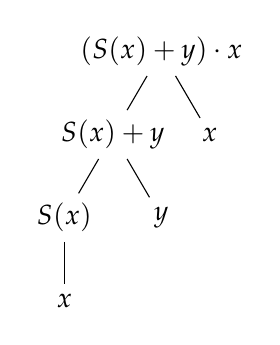
\begin{tikzpicture}[sibling distance=3.5em, level distance=3em]
  \node {$(S(x) + y)\cdot x$}
    child { node {$S(x)+y$} 
      child {node {$S(x)$}
      		child {node {$x$}}
      	}
      child {node {$y$}} }
    child { node {$x$} };
\end{tikzpicture}
\caption{A formation tree of the term $(S(x) + y)\cdot x$.}
\end{marginfigure}

The simplest type of formulas are the atomic formulas. These are only relations applied to terms. More formally, an \emph{atomic formula of a language $L$} is an expression $R(t_1, \dots, t_n)$, where $R$ is a relation symbol in $L$ and $t_1, \dots, t_n$ are terms of $L$. The set of all atomic formulas of a language $L$ is denoted as $\AFm_L$. Similarly to terms, atomic formulas can also be represented using formation trees from the formation trees of its terms and for binary relations, we use the infix notation, e.g. $\leq(x, y)$ can be written as $(x \leq y)$. For example $(x + y) = 0$, or $R(f(x), g(y,z), x)$ are atomic formulas ($f$ is a unary function, $g$ and $+$ are binary functions, and $R$ is a ternary relation).

We can finally define formulas in first-order language. The definition is similar to the one in propositional language, but this time the propositional variables are represented by atomic formulas and we additionally have the quantifiers. Formally, a \emph{formula of a language $L$} is defined inductively by
\begin{enumerate}
  \item Every atomic formula is a formula
  \item If $\varphi$ and $\psi$ are formulas, $(\varphi \to \psi), (\varphi \land \psi), (\varphi \lor \psi), (\varphi \lequiv \psi), (\neg \varphi)$ are also formulas.
  \item If $\varphi$ is a formula and $x \in \SVar$ is a variable, then $((\forall x)\varphi)$ and $((\exists x)\varphi)$ are formulas.
  \item Every formula is obtained by a finite application of the steps above.
\end{enumerate}

The set of all formulas of a language $L$ is denoted by $\Fm_L$. A formula that is a part of another formula $\varphi$ is a subformula of $\varphi$. Of course, formulas can also be expressed as their formation tree. An example is on the right.

\begin{marginfigure}[-6\baselineskip]
\centering
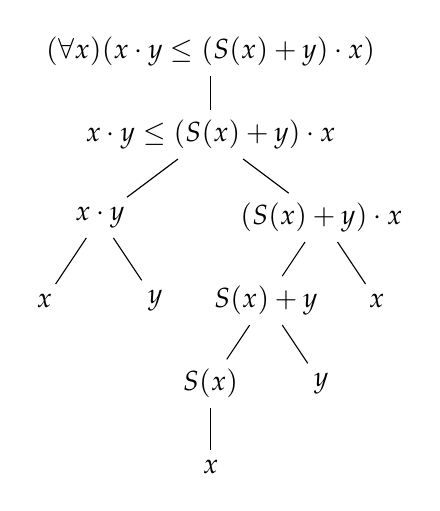
\begin{tikzpicture}[level 2/.style={sibling distance=8em}, 
                    level 3/.style={sibling distance=4em}, 
                    level distance=3em]
  \node {$(\forall x) (x \cdot y \leq (S(x) + y)\cdot x)$}
  	child {node {$x \cdot y \leq (S(x) + y)\cdot x$}
  		child {node {$x \cdot y$}
  			child {node {$x$}}
  			child {node {$y$}}
  		}
  		child {node {$(S(x) + y)\cdot x$}
  			child { node {$S(x)+y$} 
      		child {node {$S(x)$}
      			child {node {$x$}}
      		}
      	child {node {$y$}} 
      	}
      	child {node {$x$}}
      }
    };
\end{tikzpicture}
\caption{A formation tree of the formula $(\forall x) (x \cdot y \leq (S(x) + y)\cdot x)$. Moreover, $x\cdot y$ and $(S(x) + y)\cdot x$ are roots of formation trees of the terms included in the formula.}
\end{marginfigure}

As before, we can define some conventions to simplify writing the formulas. After introducing priorities of binary function symbols ($+, \cdot, \dots$) we can omit parenthesis in the infix notation of terms that are around a subterm formed by a symbol of higher priority. We also introduce the priority of logical connectives similar to the priorities in the propositional logic. The negation and quantifiers ($\neg, (\forall x), (\exists x)$) have the highest priorities, then we have conjunction and disjunction ($\land, \lor$) and, finally, the implication and equivalence ($\to, \lequiv$) have the lowest priority. Now, we can omit some of the parenthesis in the formulas.

In predicate logic, there is an important difference between so called free and bound (occurrences of) variables, as we deal with each type differently in the semantics. For a formula $\varphi$ and variable $x$, an \emph{occurrence of $x$ in $\varphi$} is a leaf labeled by $x$ in the formation tree of $\varphi$. The occurrence of $x$ in $\varphi$ is \emph{bound}, if it is in some subformula $\psi$ that starts with $(\forall x)$ or $(\exists x)$. Otherwise the occurrence is \emph{free}. A \emph{variable is free} in a formula, if it has at least one free occurrence in the formula and it is \emph{bound} if it has at least one bound occurrence. A variable can be both free and bound at the same time. For example, in the formula $x > 0 \lor (\forall x) (\exists y)(x > y)$ the variable $x$ is both free and bound, as its first occurrence is free and the second one is bound. We will use the notation $\varphi(x_1, \dots, x_n)$ to denote that $x_1, \dots, x_n$ are all the free variables in $\varphi$.

A formula is \emph{open}, if it contains no quantifiers. The set of all open formulas in a language $L$ will be denoted as $\OFm_L$. Obviously, $\AFm_L \subsetneq \OFm_L \subsetneq \Fm_L$. On the other hand, a formula is \emph{closed (a sentence)} if it has no free variables. A formula can be both closed and open at the same time, all terms of such formulas are ground terms.

In mathematics, we very often have general theorems and we later use them with a more specific substitutions. This can more formally be expressed by substituting terms for free variables in formulas, however, we need to be careful, as in some cases the substitution can change the meaning of the formula. For example, if we substituted the term $y$ for $x$ in $(\exists y) (x+y=1)$, we would change the original meaning of the formula ``there is a $y$ such that $y = 1-x$'' to a new meaning that says ``y is divisible by 2''. We want to avoid such situation while performing the substitution. Therefore, we define a term $t$ is \emph{substitutable} for a variable $x$ in a formula $\varphi$, if after the substitution of $t$ for all free occurrences of $x$, none of the variables of $t$ become bound in $\varphi$. The new formula is denoted as $\varphi(x/t)$ and we call it an \emph{instance of the formula $\varphi$} after a substitution of term $t$ for variable $x$. Alternatively, we can also define that $t$ is not substitutable for $x$ in $\varphi$ if $x$ has a free occurrence in a subformula of the form $(\exists y)\psi$ or $(\forall y) \psi$ for some variable $y$ in $t$.

We can also rename the quantified variables, but we again need to be careful. In this case, we would like to obtain an equivalent formula. Let $(Qx)\psi$ be a subformula of $\varphi$ where $Q$ is either $\forall$ or $\exists$ and $y$ is a variable. Then, if $y$ is substitutable for $x$ in $\psi$ and $y$ is not free in $\psi$, we can replace the subformula $(Qx)\psi$ with $(Qy)\psi(x/y)$ to obtain a \emph{variant} of $\varphi$ in subformula $(Qx)\psi$. A variant of $\varphi$ is obtained by variation of one or more subformulas of $\varphi$.

\informal{Creating variants in predicate logic serves some important purposes. One of them is, that we can easily transform any formula with a variable that is both free and bound into its variant, where each variable is ``pure'', i.e. only free or only bound. Moreover, we will very often create variants from formulas in order to fulfill assumptions such as ``variable $x$ is not free in $\varphi$''.}

\section{Semantics of first-order logic}

In propositional logic, models were defined as truth assignments. The truth assignment was enough to tell whether a proposition is true or false. In predicate logic, the situation is a bit more complex. First of all, the values of variables can be taken from a larger set than only $\{0,1\}$. Moreover, we need to define, what all the functions and relations mean. A natural representation of models in first-order logic is a mathematical structure. A structure is a set and a definition of functions and relations on this set. 

More formally, if we have a signature of a language $L = \langle \mathcal{R}, \mathcal{F} \rangle$ and a non-empty set $A$, a \emph{realization (interpretation) of a relation symbol} $R \in \mathcal{R}$ on the set $A$ is any relation $R^A \subseteq A^{\ar(R)}$. A realization of $=$ is the identity relation on $A$, i.e. $\mathrm{Id}_A = \{(x, x) | x \in A\}$. \emph{A realization (interpretation) of a function symbol} $f \in \mathcal{F}$ is any function $f^A: A^{\ar(f)} \to A$. Specifically, a realization of a constant symbol is some element of $A$. A \emph{structure for the language $L$} ($L$-structure) is a triple $\mathcal{A} = \langle A, \mathcal{R}^A, \mathcal{F}^A \rangle$, where $A$ is a non-empty set called the domain of the structure $\mathcal{A}$, $\mathcal{R}^A$ is a collection of realizations of the relation symbols on $A$, and $\mathcal{F}^A$ is a collection of realizations of function symbols on $A$. A structure of the language is also called a model of the language, and the class of all models of a language $L$ will be denoted as $M(L)$.

You probably already know different mathematical structures from other parts of mathematics, for example:
\begin{enumerate}
	\item $S = \struct{S, \leq}$ is an ordered set, where $\leq$ is reflexive, antisymmetric, and transitive binary relation,
	\item $G = \struct{V, E}$ is a graph,
	\item $\Int_p = \struct{\Int_p, +, -, 0}$ is the additive group of integers modulo $p$,
	\item $\Rat = \struct{\Rat, +, -, 0, 1}$ is the field of rational numbers,
	\item $\mathcal{P}(X) = \struct{\mathcal{P}(X), \setminus, \cap, \cup, \emptyset, X}$ is the set algebra over $X$, and
	\item $\Nat = \struct{\Nat, S, +, \cdot, 0, \leq}$ is the standard model of arithmetic.
\end{enumerate}
But also many other objects can be defined as structures, e.g. the finite automata or even databases.

We now aim to define the truth value of formulas in first-order logic. We already know, that a formula is constructed from atomic formulas, which are in turn constructed from terms. Therefore, in order to define the truth value of a formula, we need to start with the definition of the value of a term. Let $t$ be a term of $L = \struct{\cR, \cF}$ and $\cA = \struct{A, \cR^A, \cF^A}$ an $L$-structure. A \emph{variable assignment} over the domain $A$ is a function $e: \SVar \to A$. The \emph{value $t^A[e]$ of the term $t$} in the structure $\cA$ with respect to the assignment $e$ is defined inductively by 
\begin{enumerate}
	\item $x^A[e] = e(x)$, for $x \in \SVar$,
	\item $(f(t_1, \dots, t_n))^A[e] = f^A(t_1^A[e], \dots, t_n^A[e])$ for $f \in \cF$.
\end{enumerate}
For a constant symbol $c^A[e] = c^A$, i.e. the values of constants do not depend on the assignment $e$, and therefore also the value of ground terms does not depend on the assignment. Obviously, the value of a term $t$ depends only on the assignment of variables in $t$.

We now know, how to compute the values of individual terms, therefore, we can define the value of atomic formulas. Contrary to the values of terms, values of formulas are always from the set $\{0,1\}$. Let $\varphi$ be an atomic formula of $L = \struct{\cR, \cF}$ in the form $R(t_1, \dots, t_n)$, $\cA = \struct{A, \cR^A, \cF^A}$ is an $L$-structure and $e$ a variable assignment over $A$. The \emph{value $H^A_{at}(\varphi)[e]$ of the atomic formula $\varphi$} in the structure $\cA$ with respect to $e$ is $$H^A_{at}(\varphi)[e] = \twopartdefotherwise{1}{(t_1^A[e], \dots t_n^A[e]) \in R^A}{0}$$

Specifically, for the equality relation $=$, the only possible realization is $\mathrm{Id}_A$ and therefore $H^A_{at}(t_1=t_2)[e] = 1$, if $t_1^A[e]=t_2^A[e]$ and $0$ otherwise. We can again see that the value of a formula depends only on the assignment of variables in the formula and that the value of a ground formula does not depend on the assignment at all.

We can finally define the value of a general formula. The definition is quite long, but also very similar to the one in propositional logic. In fact, the only difference is in the last two cases. The atomic formulas in this case play the role of the propositional variables.

The value $H^A(\varphi)[e]$ of formula $\varphi$ in the structure $A$ with respect to $e$ is 
\begin{align*}
	H^A(\varphi)[e] & = H^A_{at}(\varphi)[e] \text{ if } \varphi \text{ is atomic} \\
	H^A(\neg \varphi)[e] & = -_1(H^A(\varphi)[e])\\
	H^A(\varphi \land \psi)[e] & = \land_1(H^A(\varphi)[e], H^A(\psi)[e])\\
	H^A(\varphi \lor \psi)[e] & = \lor_1(H^A(\varphi)[e], H^A(\psi)[e])\\
	H^A(\varphi \to \psi)[e] & = \to_1(H^A(\varphi)[e], H^A(\psi)[e])\\
	H^A(\varphi \lequiv \psi)[e] & = \lequiv_1(H^A(\varphi)[e], H^A(\psi)[e])\\
	H^A((\forall x)\varphi)[e] & = \min_{a \in A}(H^A(\varphi)[e(x/a)])\\
	H^A((\exists x)\varphi)[e] & = \max_{a \in A}(H^A(\varphi)[e(x/a)])
\end{align*}
where $-_1, \land_1, \lor_1, \to_1, \lequiv_1$ are the functions given by the truth tables in the part on propositional logic and $e(x/a)$ is an assignment  assigning value $a$ to variable $x$ and otherwise identical to $e$. We can see that the value of a formula depends only on the assignment of free variables in the formula (we check all possible assignments for the bound variables in steps 7 and 8).

The structure $\cA$ satisfies the formula $\varphi$ if $H^A(\varphi) = 1$, we denote the fact as $\cA \vDash \varphi[e]$, otherwise we write $\cA \nvDash \varphi[e]$. We can easily check that all the following hold
\begin{align*}
\cA \vDash \neg \varphi[e] & \Leftrightarrow \cA \nvDash \varphi[e] \\
\cA \vDash (\varphi \land \psi)[e] & \Leftrightarrow \cA \vDash \varphi[e] \text{ and } \cA \vDash \psi[e]\\
\cA \vDash (\varphi \lor \psi)[e] & \Leftrightarrow \cA \vDash \varphi[e] \text{ or } \cA \vDash \psi[e]\\ 
\cA \vDash (\varphi \to \psi)[e] & \Leftrightarrow \cA \vDash \varphi[e] \text{ implies } \cA \vDash \psi[e]\\
\cA \vDash (\varphi \lequiv \psi)[e] & \Leftrightarrow \cA \vDash \varphi[e] \text{ if and only if } \cA \vDash \psi[e]\\
\cA \vDash (\forall x)(\varphi)[e] & \Leftrightarrow \cA \vDash \varphi[e(x/a)] \text{ for every } a \in A \\
\cA \vDash (\exists x)(\varphi)[e] & \Leftrightarrow \cA \vDash \varphi[e(x/a)] \text{ for some } a \in A
\end{align*}
Furthermore, if $t$ is substitutable for $x$ in $\varphi$, then for every structure $\cA$ and assignment $e$, $\cA \vDash \varphi(x/t)[e]$ if and only if $\cA \vDash \varphi[e(x/a)]$, where $a = t^A[e]$. If $\psi$ is a variant of $\varphi$ then $\cA \vDash \varphi[e]$ if and only if $\cA \vDash \psi[e]$.

As in propositional logic, we can generalize the notion above to validity in structure and in theory. Let $\varphi$ be a formula of a language $L$, and $\cA$ an $L$-structure. We say, that \emph{$\varphi$ is valid in $\cA$}, denoted as $\cA \vDash \varphi$, if $\cA \vDash \varphi[e]$ for every $e: \SVar \to A$. We also say that \emph{$\cA$ satisfies $\varphi$}. Otherwise, we write $\cA \nvDash \varphi$. The formula \emph{$\varphi$ is contradictory in $\cA$} if $\cA \vDash \neg \varphi$, i.e. if $\cA \nvDash \varphi[e]$ for every $e$.

We can easily check, that for any structure $\cA$ and formulas $\varphi, \psi$ the following holds:
\begin{align}
	\cA \vDash \varphi & \Rightarrow \cA \nvDash \neg \varphi \\
	\cA \vDash \varphi \land \psi & \Leftrightarrow \cA \vDash \varphi \text{ and } \cA \vDash \psi\\
	\cA \vDash \varphi \lor \psi & \Leftarrow \cA \vDash \varphi \text{ or } \cA \vDash \psi\\
	\cA \vDash \varphi & \Leftrightarrow \cA \vDash (\forall x)\varphi
\end{align}
Moreover, if $\varphi$ and $\psi$ are sentences, the implications in (1) and (3) are in fact equivalences. The last equivalence (4) also shows, that $\cA \vDash \varphi$ if and only if $\cA \vDash \psi$, where $\psi$ is the \emph{universal closure} of $\varphi$, i.e. the formula $(\forall x_1)(\forall x_1) \dots (\forall x_n)\varphi$, where $x_1, \dots, x_n$ are all the free variables of $\varphi$.

A \emph{theory} of a language $L$ is any set $T$ of formulas of $L$ (the \emph{axioms} of the theory). A \emph{model of a theory $T$} is an $L$-structure $\cA$ such that $\cA \vDash \varphi$ for every $\varphi \in T$. We also write $\cA \vDash T$ and say that $\cA$ satisfies $T$. The \emph{class of all models} of theory $T$ is $M(T) = \{\cA \in M(L) | \cA \vDash T\}$. A formula is \emph{valid in $T$} (true in $T$) ($T\vDash \varphi$) if $\cA \vDash \varphi$ for every model $\cA$ of $T$. Otherwise we write $T \nvDash \varphi$. A formula \emph{$\varphi$ is contradictory in $T$} if $T \vDash \neg \varphi$ and \emph{$\varphi$ is independent in $T$} if it is neither valid nor contradictory in $T$. For empty theory $T$, we can omit $T$ in the notation and $M(T)=M(L)$. In this case, ($\vDash \varphi$) means that the formula $\varphi$ is \emph{logically valid} (\emph{a tautology}). A \emph{consequence of $T$} is the set $\theta^L(T)$ of all sentences of $L$ valid in $T$, i.e. $$\theta^L(T) = \{\varphi \in \Fm_L\ | T\vDash \varphi \text{ and } \varphi \text{ is a sentence}\}\,.$$

\informal{The definitions above should closely resemble those we saw in propositional logic, the main difference is in the definition of the model. In propositional logic, we could use truth assignments, while in predicate logic, the model is a structure. The structure, and its definitions of functions and relations in fact give the truth values to the atomic formulas. The atomic formulas then play the role of the propositional variables. Of course, in predicate logic, we also need to take care of the quantifiers, which brings another complexity to the definitions.}

For example, the theory of orderings $T$ is a theory in language $L=\struct{\leq}$ with axioms
\begin{align*}
	x \leq x & & \text{reflexivity,} \\
	x \leq y \land y \leq x \to x = y & & \text{antisymmetry,} \\
	x \leq y \land y \leq z \to x \leq z & & \text{transitivity.} \\
\end{align*}

The models of $T$ (ordered sets) are structures $\struct{S, \leq_S}$. For example $\mathcal{A} = \struct{\Nat, \leq}$ or $\mathcal{B} = \struct{\mathcal{P}(X), \subseteq}$ for a set $X = \{0,1,2\}$. The formula $\varphi \equiv x \leq y \lor y \leq x$ is valid in $\cA$, but not in $\mathcal{B}$, as $\mathcal{B} \nvDash \varphi[e]$ for $e(x) = \{0\}$ and $e(y)=\{1\}$, therefore it is independent in $T$. The sentence $\psi \equiv (\exists x)(\forall y)(y \leq x)$ is valid in $\mathcal{B}$ and contradictory in $\cA$, and therefore also independent in $T$. Finally, the formula $\chi \equiv (x \leq y \land y \leq z \land z \leq x) \to (x = y \land y = z)$ is valid in $T$, denoted as $T \vDash \chi$.

We say that a theory $T$ in a language $L$ is \emph{semantically inconsistent} if $T \vDash \bot$, otherwise \emph{$T$ is consistent}. The theory \emph{$T$ is complete}, if it is consistent, and every sentence of $L$ is either valid or contradictory in $T$. The $L$-theory \emph{$T$ is an extension} of another theory $T'$ in language $L'$ if $L' \subseteq L$ and $\theta^{L'}(T') \subseteq \theta^L(T)$. The \emph{extension is simple}, if $L' = L$ and it is \emph{conservative} if $\theta^{L'}(T') = \theta^L(T) \cap \Fm_{L'}$. The \emph{two theories are equivalent}, if one is the extension of the other and vice versa.

We also define a form of equivalence for two structures -- we say that two $L$-structures $\cA, \cB$ are \emph{elementarily equivalent}, denoted as $\mathcal{A} \equiv \mathcal{B}$ if they satisfy the same sentences of $L$. It means that we cannot write a sentence in the language that would make any distinction between the two structures. Later, we will also define the isomorphism of structures and we will see that it is a stronger property, i.e. that any two isomorphic structures are elementarily equivalent, but not vice versa.

The definitions above lead to a simple observation -- a theory $T$ of language $L$ is consistent if it has a model. It is complete if and only if it has a single model, up to elementary equivalence. The theory $T$ is an extension of another theory $T'$ in the same language $L$ if and only if $M(T) \subseteq M(T')$ and the theories are equivalent if $M(T) = M(T')$.

We can transform the problem of validity in a theory into the problem of satisfiability of another theory, similarly to the proof by contradiction. For every theory $T$ and sentence $\varphi$ (in the same language), it holds $T \cup \{\neg \varphi\}$ is unsatisfiable if and only if $T \vDash \varphi$. Why? Because by the definitions, $T \cup \{\neg \varphi\}$ is unsatisfiable (i.e. has no model) if $\neg \varphi$ is not valid in any model of $T$, which means (and here we need the assumption that $\varphi$ is a sentence) that $\varphi$ is valid in every model of $T$ and that in turn means $T \vDash \varphi$. 

You also probably know the notion of substructure from other parts of mathematics. Let $\cA = \struct{A, \cR^A, \cF^A}$ and $\mathcal{B} = \struct{B, \cR^B, \cF^B}$ be structures for $L = \struct{\cR, \cF}$. We say that \emph{$\mathcal{B}$ is an (induced) substructure of $\cA$} ($\mathcal{B} \subseteq \cA$) if $B \subseteq A$, $R^B = R^A \cap B^{\ar(R)}$ for every $R \in \cR$, and $f^B = f^A \cap (B^{\ar(f)}\times B)$ for every $f \in \cF$. A set $C$ is a domain of some substructure of $\cA$ if and only if it is closed under all functions of $\cA$\sidenote{A set $C \subseteq A$ is closed under a function $f: A^{\ar(f)} \to A$, if $f(x_1, \dots, x_{ar(f)}) \in C$ for all $x_1, \dots, x_{\ar(f)} \in C$.}. The representative substructure is then called a \emph{restriction of $\cA$ to $C$} and denotes as $\cA \restrict C$.

If we have a structure $\cA$, its substructure $\mathcal{B}$ in a language $L$ and a value assignment $e: \SVar \to B$, then, obviously, for an open formula $\varphi$, $\cA \vDash \varphi[e]$ if and only if $\mathcal{B} \vDash \varphi[e]$. The essential fact here is that $e$ assigns only values from $B$ and therefore the values of the terms are the same in both $\cA$ and $\mathcal{B}$. The same then holds for the atomic formulas and by induction on the complexity of the formula also for general formulas. This simple observation however has an interesting corollary. For every open formula $\varphi$ and a structure $\cA$, the formula is valid in the structure $\cA$ if and only if it is valid in every substructure $\mathcal{B}$ of $\cA$. If a theory $T$ contains only open axioms (so called \emph{open theory}), this implies that every substructure of a model of $T$ is also a model of $T$.

The last observation is important in case we want to check, whether a theory $T$ is openly axiomatizable, i.e. if there is an equivalent theory $T'$ that contains only open axioms. In such a case, we just need to check, if every substructure of a model of the theory $T$ is also a model of $T$. If it is, then $T$ is openly axiomatizable, otherwise it is not.

Let $\cA = \struct{A, \cR^A, \cF^A}$ be a structure and $X \subseteq A$. Let $B$ be the smallest subset of $A$ containing $X$ and closed under all functions of $\cA$ (including constants). Then the structure $\cA \restrict B$ is denoted as $\cA\langle X \rangle$ and is called \emph{a substructure of $\cA$ generated by the set $X$}. 

Let $\cA$ be a structure for the language $L$ and $L'\subseteq L$. By omitting realizations of symbols that are not in $L'$ we obtain a structure $\cA'$ in $L'$ called the \emph{reduct of $\cA$ to the language $L'$}. The structure $\cA$ is then called the expansion of $\cA'$ into $L$.

\chapter{Tableau method in first-order logic}

As in the propositional logic, we will use the tableau method to prove formulas in first order logic. While most of the ideas from propositional logic will be used again, the more complex structure of first-order formulas leads to additional rules in the tableau method (these are basically the atomic tableaux for the quantifiers). Also, the proofs of soundness and completeness will get more technical because we know need to also consider the structure of the terms, and because the models in first-order logic are mathematical structures rather than truth assignments. However, we will define so called canonical structure as a general structure for a language that prescribes the definitions of all function symbols, thus we will again need to define only the truth values of atomic formulas, thus reducing most of the ideas to propositional logic.

In fact, propositional logic can be seen as a fragment of the predicate logic, where we do not use the quantifiers and the propositional variables are represented by nullary predicate symbols.

In the tableau proofs in the predicate logic, we will work in a language that contains countable amount of new constants. Therefore it is important to show, that adding new constants to the language does not change the validity of formulas in the language. This should be intuitive -- adding constants without telling anything about them means we only add symbols that can be used as names of specific elements in the structure. This is more formally demonstrated by the following theorem.

\begin{theorem}
Let $\varphi$ be a formula in a language $L$ with free variables $x_1, \dots, x_n$ and let $T$ be a theory in $L$. Let $L'$ be an extension of $L$ with new constant symbols $c_1, \dots, c_n$ and let $T'$ denote the theory $T$ in $L'$. Then $$T \vDash \varphi \text{ if and only if } T'\vDash \varphi(x_1/c_1, \dots, x_n/c_n)\,.$$
\end{theorem}
\begin{proof}
($\Rightarrow$) If $\cA'$ is a model of $T'$, let $\cA$ be reduct of $\cA'$ to $L$. Since $\cA \vDash \varphi[e]$ for every assignment $e$, we have $\cA \vDash \varphi[e(x_1/c_1^{A'}, \dots, x_n/c_n^{A'})]$, i.e. $\cA' \vDash \varphi(x_1/c_1, \dots, x_n/c_n)$.

($\Leftarrow$) For the other implication, if $\cA$ is a model of $T$ and $e$ an assignment, let $\cA'$ be the expansion of $\cA$ into $L'$ by setting $c_i^{A'} = e(x_i)$ for every $i$. Since $\cA' \vDash \varphi(x_1/c_1, \dots, x_n/c_n)[e']$ for every assignment $e'$, we have $\cA' \vDash \varphi[e(x_1/c_1^{A'}, \dots, x_n/c_n^{A'})]$, i.e. $\cA \vDash \varphi[e]$.
\end{proof}

The basics of the tableau method in predicate logic are similar to the tableau method in propositional logic. A tableau is still a binary tree that represents the search for a counterexample. The nodes are still labeled with entries, i.e. formulas with a sign $T$ or $F$. However, this time, the formulas will be sentences. A branch is still contradictory if it contains $T \varphi$ and $F \varphi$ for a formula $\varphi$. A proof of a formula $\varphi$ is still a contradictory tableau with $F \varphi$ as its root entry. If a counterexample exists, there will be a non-contradictory branch in the finished tableau that provides us with the counterexample. We will again define a systematic tableau that is always finished and in case it is a proof of a formula, it is also finite. 

There are however some differences -- we need to add atomic tableaux for the logical quantifiers. In these the quantified variables will be substituted with ground terms following some rules. We extend the language by new constant symbols that act as the witnesses of the entries $T(\exists x) \varphi x$ and $F(\forall x) \varphi(x)$. In a finished non-contradictory branch for an entry $T (\forall x) \varphi(x)$, we will have the entries $T \varphi(x/t)$ for every ground term $t$ of the extended language. Similarly for $F (\forall x) \varphi(x)$ and $F \varphi(x/t)$.

We have some assumptions in the tableau method in predicate logic. First of all, the formula we want to prove needs to be a sentence. This is not a problem -- we can always prove the universal closure of a formula if it has free variables, as we already know, that these two are equivalent. Furthermore, we also assume the axioms of the theory are sentences -- but that is also not a problem, we can again take the universal closures of the axioms. We also assume that the language $L$ is countable. That also means that every theory in $L$ is countable. We define $L_C$ as the extension of $L$ by new constant symbols $c_0, c_1, \dots$. Then there are countably many ground terms of $L_C$. Let $t_i$ denote the $i$-th ground term in some fixed enumeration. Finally, we start with the assumption that $L$ is without equality, but we will deal with this one later.

\begin{figure*}[ht]
\centering
\begin{minipage}{\textwidth}
\begin{tabular}{|c|c|c|c|c|c|}
\hline
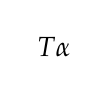
\begin{tikzpicture}[sibling distance=3em, level distance=3em]
  \node {$T \alpha$};
\end{tikzpicture} &
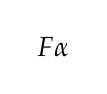
\begin{tikzpicture}[sibling distance=3em, level distance=3em]
  \node {$F \alpha$};
\end{tikzpicture} &
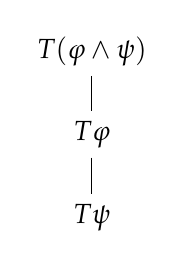
\begin{tikzpicture}[sibling distance=3em, level distance=3em]
  \node {$T (\varphi \land \psi)$}
    child { node {$T \varphi$} 
      child {node {$T \psi$}}};
\end{tikzpicture} &
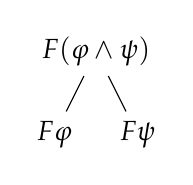
\begin{tikzpicture}[sibling distance=3em, level distance=3em]
  \node {$F (\varphi \land \psi)$}
    child { node {$F \varphi$} }
    child { node {$F \psi$}};
\end{tikzpicture} &
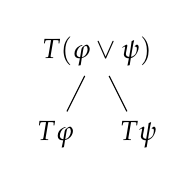
\begin{tikzpicture}[sibling distance=3em, level distance=3em]
  \node {$T (\varphi \lor \psi)$}
    child { node {$T \varphi$} }
    child { node {$T \psi$}};
\end{tikzpicture} &
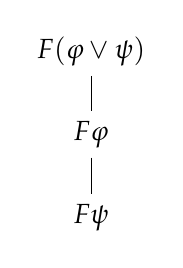
\begin{tikzpicture}[sibling distance=3em, level distance=3em]
  \node {$F (\varphi \lor \psi)$}
    child { node {$F \varphi$} 
      child {node {$F \psi$}}};
\end{tikzpicture} \\
\hline
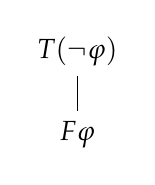
\begin{tikzpicture}[sibling distance=3em, level distance=3em]
  \node {$T (\neg \varphi)$}
    child { node {$F \varphi$} };
\end{tikzpicture} &
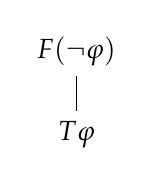
\begin{tikzpicture}[sibling distance=3em, level distance=3em]
  \node {$F (\neg \varphi)$}
    child { node {$T \varphi$} };
\end{tikzpicture} &
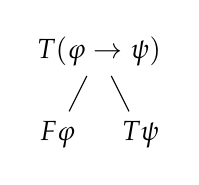
\begin{tikzpicture}[sibling distance=3em, level distance=3em]
  \node {$T (\varphi \to \psi)$}
    child { node {$F \varphi$} }
    child { node {$T \psi$}};
\end{tikzpicture} &
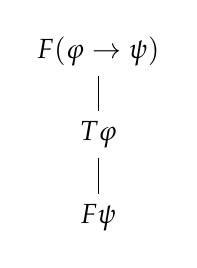
\begin{tikzpicture}[sibling distance=4em, level distance=3em]
  \node {$F (\varphi \to \psi)$}
    child { node {$T \varphi$} 
      child {node {$F \psi$}}};
\end{tikzpicture} &
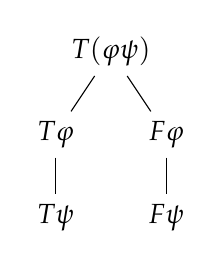
\begin{tikzpicture}[sibling distance=4em, level distance=3em]
  \node {$T (\varphi \lequiv \psi)$}
    child { node {$T \varphi$} 
    	child {node {$T \psi$}}}
    child { node {$F \varphi$} 
    	child {node {$F \psi$}}};
\end{tikzpicture} &
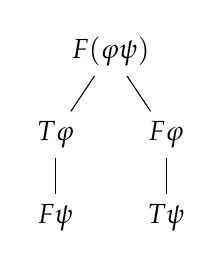
\begin{tikzpicture}[sibling distance=4em, level distance=3em]
  \node {$F (\varphi \lequiv \psi)$}
    child { node {$T \varphi$} 
    	child {node {$F \psi$}}}
    child { node {$F \varphi$} 
    	child {node {$T \psi$}}};
\end{tikzpicture} \\
\hline
\end{tabular}
\end{minipage}
\caption{The atomic tableaux for logical connectives. In the tableau, $\varphi, \psi$ are sentences and $\alpha$ are atomic sentences.}
\label{fig:pred_tableaux}
\end{figure*}

The tableaux will again be constructed from atomic tableaux. In the predicate logic, we still have the atomic tableaux for the logical connectives ($\lor, \land, \neg, \to, \lequiv$). These are essentially the same as in propositional logic, but instead of having tableaux for propositional variables, we have them for atomic sentences $\alpha$. These atomic tableaux are shown in Figure~\ref{fig:pred_tableaux}. In the tableaux, $\varphi$ and $\psi$ denote formulas in $L_C$, and $\alpha$ denotes an atomic sentence in the same language.

Additionally, we also have atomic tableaux for the quantifiers. These are shown in Figure~\ref{fig:pred_tableaux_quant}. Again, $\varphi$ represents a formula of the language $L_C$ with a free variable $x$, $t$ is any ground term of $L_C$ and $c$ is a new constant symbol from $L_C \setminus L$.

\begin{figure*}[ht]
\begin{minipage}{\textwidth}
\begin{tabular}{|c|c|c|c|}
\hline
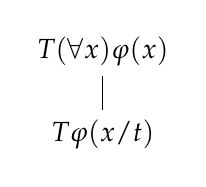
\begin{tikzpicture}[sibling distance=3em, level distance=3em]
  \node {$T (\forall x) \varphi(x)$}
  	child {node {$T \varphi(x/t)$}};
\end{tikzpicture} &
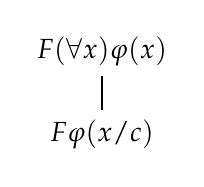
\begin{tikzpicture}[sibling distance=3em, level distance=3em]
  \node {$F (\forall x) \varphi(x)$}
  	child {node {$F \varphi(x/c)$}};
\end{tikzpicture} &
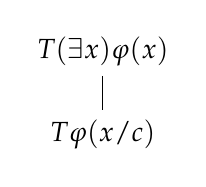
\begin{tikzpicture}[sibling distance=3em, level distance=3em]
  \node {$T (\exists x) \varphi(x)$}
  	child {node {$T \varphi(x/c)$}};
\end{tikzpicture} &
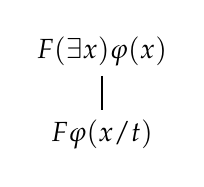
\begin{tikzpicture}[sibling distance=3em, level distance=3em]
  \node {$F (\exists x) \varphi(x)$}
  	child {node {$F \varphi(x/t)$}};
\end{tikzpicture} \\
for any term $t$ & for a new constant $c$ & for a new constant $c$ & for any term $t$ \\
\hline
\end{tabular}
\end{minipage}
\caption{The atomic tableaux for quantifiers}
\label{fig:pred_tableaux_quant}
\end{figure*}

The constant symbol $c$ represents a witness for the entry $T(\exists x)\varphi(x)$ or $F(\forall x)\varphi(x)$. These symbols must be new, i.e. not used anywhere else on the same branch in the tableau and also cannot be from the language $L$, as we do not want to assume anything about their value.

A \emph{tableau from a theory $T$} is again a sequence $\tau_0, \tau_1, \dots$ of finite tableaux from $T$, such that $\tau_{i+1}$ is formed from $\tau_i$ by steps 2 or 3 bellow, formally $\tau=\cup \tau_n$.

A \emph{finite tableau from a theory $T$} is a binary tree labeled with entries defined inductively as
\begin{enumerate}
 \item every atomic tableau from $T$ is a finite tableau from $T$, in cases $F(\forall x) \varphi(x)$ and $T(\exists x)\varphi(x)$ we may use any constant symbol $c \in L_C \setminus L$;
 \item if $P$ is an entry on a branch $V$ in a finite tableau from $T$ then by adjoining the atomic tableau from $P$ at the end of the branch $V$ we obtain a finite tableau from $T$, in cases $F(\forall x) \varphi(x)$ and $T(\exists x)\varphi(x)$ we may only use constant symbols $c \in L_C \setminus L$ that does not appear on $V$;
 \item if $V$ is a branch in a finite tableau from $T$ and $\varphi \in T$, then by adjoining $T \varphi$ at the end of $V$ we obtain a finite tableau from $T$; and
 \item every finite tableau is formed by finitely many steps above.
\end{enumerate}

Similarly to the tableau method in propositional logic, we do not need to repeat the entry that is expanded again on the branch. However, we have to repeat it in cases the entry is $T(\forall x) \varphi(x)$, or $F(\exists x)\varphi(x)$. This convention is demonstrated in the tableaux in Figure~\ref{fig:tableau_convention}.

\begin{figure}[ht]
\begin{minipage}{0.5\textwidth}
\centering
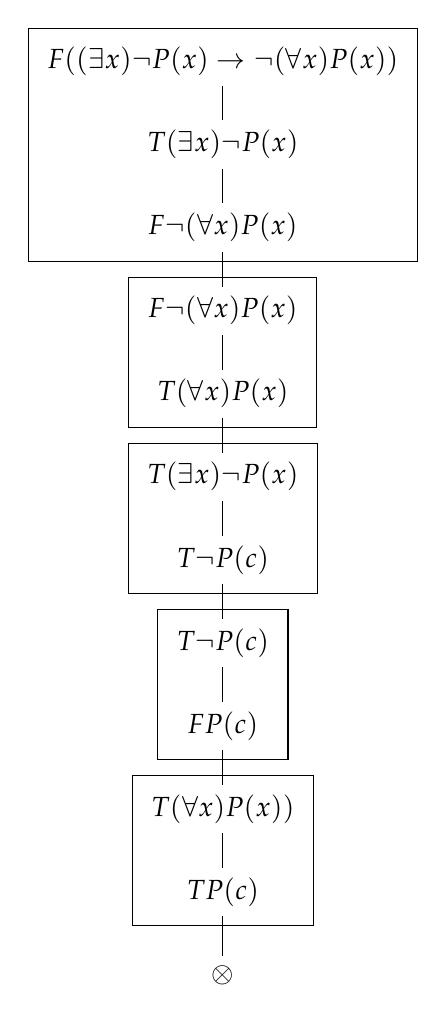
\begin{tikzpicture}[sibling distance=4em, level distance=3em]
  \node(n) {$F((\exists x)\neg P(x) \to \neg (\forall x)P(x))$}
    child { node {$T (\exists x)\neg P(x)$} 
    	child { node {$F \neg (\forall x)P(x)$} 
    		child {node {$F \neg (\forall x)P(x)$}
    			child {node {$T (\forall x)P(x)$}
    				child {node {$T (\exists x)\neg P(x)$}
	    				child {node {$T\neg P(c)$}
	    					child {node {$T\neg P(c)$}
	    						child {node {$F P(c)$}
	    							child {node {$T (\forall x)P(x))$}
	    								child {node {$T P(c)$}
	    									child {node {$\otimes$}}
	    								}
	    							}
	    						}
	    					}
	    				}
	    			}
    			}
    		}
    	}
    };
  \node[fit=(n)(n-1-1), draw] {};
  \node[fit=(n-1-1-1)(n-1-1-1-1), draw] {};
  \node[fit=(n-1-1-1-1-1)(n-1-1-1-1-1-1), draw] {};
  \node[fit=(n-1-1-1-1-1-1-1)(n-1-1-1-1-1-1-1-1), draw] {};
  \node[fit=(n-1-1-1-1-1-1-1-1-1)(n-1-1-1-1-1-1-1-1-1-1), draw] {};
\end{tikzpicture}
\end{minipage}
\begin{minipage}{0.5\textwidth}
\centering
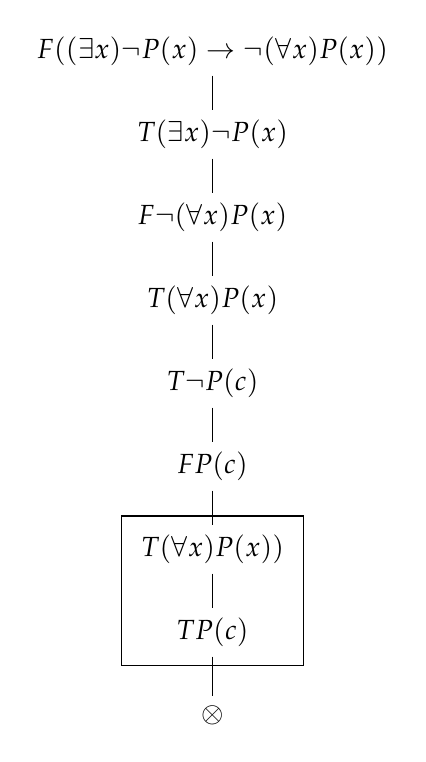
\begin{tikzpicture}[sibling distance=4em, level distance=3em]
  \node(n) {$F((\exists x)\neg P(x) \to \neg (\forall x)P(x))$}
    child { node {$T (\exists x)\neg P(x)$} 
    	child { node {$F \neg (\forall x)P(x)$} 
  			child {node {$T (\forall x)P(x)$}
					child {node {$T\neg P(c)$}
						child {node {$F P(c)$}
							child {node {$T (\forall x)P(x))$}
								child {node {$T P(c)$}
									child {node {$\otimes$}}
								}
							}
						}
					}
    		}
    	}
    };
    \node[fit=(n-1-1-1-1-1-1)(n-1-1-1-1-1-1-1), draw] {};
\end{tikzpicture}
\end{minipage}
\caption{Example tableau. The rectangles on the left show the atomic tableaux used. The version on the right removes the repeated entries that can be removed, the entry in the rectangle in the right tableau must be repeated. $c$ is a new constant symbol where it first appears in the tableau, and in the last step, we chose $c$ as the term in the atomic tableau for $T(\forall x)P(x)$. The symbol $\otimes$ denotes a contradictory branch.}
\label{fig:tableau_convention}
\end{figure}

\informal{The cases where we need to repeat the entry are those where we can choose any term in the atomic tableau and if we chose incorrectly, we want to have another attempt to guess correctly. By repeating the entry on the branch, we have another non-reduced entry of the same type that we will reduce later.}

A \emph{branch $V$ is contradictory} if it contains entries $T \varphi$ and $F \varphi$ for some sentence $\varphi$, otherwise it is noncontradictory. A tableau $\tau$ is contradictory if all its branches are contradictory. A \emph{tableau proof of a sentence $\varphi$ from $T$} is a contradictory tableau from $T$ with $F \varphi$ in the root. $T \vdash \varphi$ denotes that $\varphi$ is tableau provable from $T$. A \emph{refutation of a sentence $\varphi$ by a tableau from $T$} is a contradictory tableau from $T$ with $T \varphi$ in the root. A sentence is tableau refutable if there is a tableau refutation of the sentence.

Compared to the propositional version of the tableau method, the definition of a finished tableau is a bit more complicated -- we need to account for the cases where we need to guess the correct terms and such atomic tableaux must be in the tableau for all the ground terms of $L_C$. This is reflected in the definition of the reduced entry. An occurrence on an entry $P$ in a node $v$ of a tableau $\tau$ is $i$-th if $v$ has exactly $i-1$ predecessors labeled by $P$. The \emph{occurrence of $P$ is reduced}, if $P$ is neither of in form $T(\forall x)\varphi(x)$ nor $F(\exists x)\varphi(x)$ and $P$ occurs in $V$ as a root of an atomic tableau (it was already expanded on $V$); or if $P$ is in form $T(\forall x)\varphi(x)$ or $F(\exists x)\varphi(x)$, $P$ has an $(i+1)$-th occurrence on $V$ and $V$ contains an entry $T \varphi(x/t_i)$ or $F \varphi(x/t_i)$, where $t_i$ is the $i$-th ground term in $L_C$ (in some enumeration of ground terms). Now, let $V$ be a branch in a tableau $\tau$ from a theory $T$. We say that $V$ is finished if it is contradictory, or every occurrence of an entry on $V$ is reduced on $V$, and moreover $V$ contains $T \varphi$ for every $\varphi \in T$. A tableau $\tau$ is finished if every branch in $\tau$ is finished.

We can now define the systematic tableau in predicate logic. The systematic tableau is again always finished and, moreover, if it is a proof, it is finite, as we shall see later. Let $R$ be an entry and $T=\{\varphi_0, \varphi_1, \dots\}$ a theory. The systematic tableau for $R$ from $T$ is the result $\tau = \cup \tau_n$ of the following construction:
\begin{enumerate}
  \item $\tau_0$ is the atomic tableau for $R$. In case $R$ is of the form $T(\exists x)\varphi(x)$ or $F(\forall x) \varphi(x)$ we take $c_0$ as the new constant. In case $R$ is of form $T(\forall x) \varphi(x)$ or $F(\exists x) \varphi(x)$ we take $t_1$ as the term.
  \item Let $v$ be the leftmost node in the smallest level as possible in tableau $\tau_n$ containing an occurrence of an entry $P$ that is not reduced on some noncontradictory branch through $v$.
  \item If $P$ is neither $T(\forall x)\varphi(x)$ nor $F(\exists x)\varphi(x)$, let $\tau'_n$ be the tableau obtained from $\tau_n$ by adjoining the atomic tableau for $P$ to every noncontradictory branch through $v$. In case $P$ is in the form $T(\exists x)\varphi(x)$ or $F(\forall x) \varphi(x)$, we take $c_i$ as the new constant for lowest possible $i$.
  \item If $P$ is either $T(\forall x)\varphi(x)$ or $F(\exists x)\varphi(x)$ and it has the $i$-th occurrence in $v$, let $\tau'_n$ be the tableau obtained from $\tau_n$ by adjoining the atomic tableau for $P$ to every noncontradictory branch through $v$, where we take the term $t_i$ for $t$.
  \item Let $t_{n+1}$ be the tableau obtained from $\tau'_n$ by adjoining $T \varphi_n$ to every noncontradictory branch that does not contain $T \varphi_n$ yet.
\end{enumerate}  

An example of a systematic tableau is shown in Figure~\ref{fig:tableau_systematic}.

\begin{figure}[t]
\centering
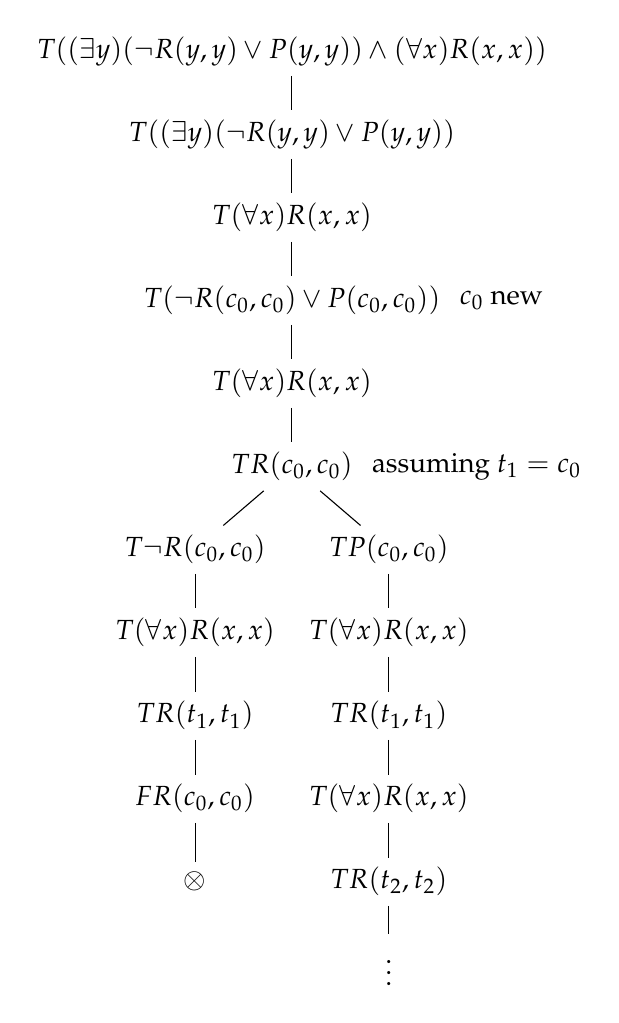
\begin{tikzpicture}[sibling distance=7em, level distance=3em]
  \node(n) {$T((\exists y)(\neg R(y,y) \lor P(y,y)) \land (\forall x)R(x,x))$}
    child { node {$T((\exists y)(\neg R(y,y) \lor P(y,y))$} 
    	child { node {$T(\forall x)R(x,x)$} 
    		child {node [label=right:{$c_0$ new}] {$T(\neg R(c_0,c_0) \lor P(c_0,c_0))$}
    			child {node {$T(\forall x)R(x,x)$}
    				child {node [label=right:{assuming $t_1 = c_0$}]{$TR(c_0,c_0)$}
	    				child {node {$T\neg R(c_0, c_0)$}
	    					child {node {$T(\forall x)R(x,x)$}
	    						child {node {$TR(t_1, t_1)$}
	    							child {node {$FR(c_0, c_0)$}
	    								child {node {$\otimes$}}
	    							}
	    						}
	    					}
	    				}
	    				child {node {$TP(c_0, c_0)$}
	    					child {node {$T(\forall x)R(x,x)$}
	    						child {node {$TR(t_1, t_1)$}
	    							child {node {$T(\forall x)R(x,x)$}
	    								child {node {$TR(t_2, t_2)$}
	    									child {node {$\vdots$}}
	    								}
	    							}
	    						}
	    					}
	    				}
	    			}
    			}
    		}
    	}
    };
\end{tikzpicture}
\caption{An example of a systematic tableau. The left branch is contradictory, while the right one is noncontradictory and finished but infinite.}
\label{fig:tableau_systematic}
\end{figure}


As in propositional logic, every systematic tableau is finished. We can show this using the same method as in propositional logic. Let $\tau = \cup \tau_n$ be a systematic tableau from $T = \{\varphi_0, \varphi_1, \dots\}$ with a root entry $R$ and let $P$ be an entry in a node $v$ of the tableau $\tau$. There are only finitely many entries in levels above $v$, therefore if the occurrence of $P$ in $v$ was unreduced, it would be eventually found in step 2, and reduced in steps 3 or 4 of the construction above. The step 4 above ensures that for every $\varphi_n \in T$, $T \varphi_n$ is in the tableau no later than in $\tau_{n+1}$ on every noncontradictory branch. Therefore, all the branches in the tableau are finished.

We can also easily show that, if a systematic tableau $\tau$ is a proof (from a theory $T$), it is finite. Assume that $\tau$ is infinite, then by the König's lemma it contains an infinite branch. But this branch is noncontradictory, since we prolong only noncontradictory branches in the construction. But that is a contradiction with $\tau$ being a proof as proofs are contradictory tableaux.

Up until now, we have discussed tableau method only in languages without equality, however, the principles are the same in languages with equality, we just need to add the equality axioms into the theory. The \emph{equality axioms for language $L$} are 
\begin{enumerate}
	\item $x=x\,,$
	\item $x_1 = y_1 \land \dots \land x_n=y_n \to f(x_1, \dots, x_n) = f(y_1, \dots y_n)$ for every $n$-ary function symbol $f$ in $L\,,$ and
	\item $x_1 = y_1 \land \dots \land x_n=y_n \to (R(x_1, \dots, x_n) \to R(y_1, \dots y_n))$ for every $n$-ary relation symbol $R$ in $L$ (including ``='').
\end{enumerate}
The tableau proof from a theory $T$ in language $L$ with equality is a tableau proof from $T^*$ where $T^*$ denotes the extension of $T$ by adding the axioms of equality for $L$.

The problem is that the extended theory $T^*$ can have models, where equality is represented by a relation $=^A$ which is different from identity. This can be solved by considering the quotient structures by $=^A$ of these models. Let $\sim$ be an equivalence on $A$, $f: A \to A^n$, and $R\subseteq A^n$ for $n \in \Nat$. Then $\sim$ is a \emph{congruence for the function $f$} if for every $x_1, \dots, x_n, y_1, \dots, y_n \in A: x_1 \sim x_2 \land \dots \land x_n \sim y_n \Rightarrow f(x_1, \dots, x_n) \sim{=} f(y_1, \dots, y_n)$, and it is a \emph{congruence for the relation $R$} if for every $x_1, \dots, x_n, y_1, \dots, y_n \in A: x_1 \sim x_2 \land \dots \land x_n \sim y_n \Rightarrow R(x_1, \dots, x_n) \Leftrightarrow R(y_1, \dots, y_n)$. 

Let an equivalence $\sim$ in $A$ is a congruence for every function and relation in a structure $\cA = \struct{A, \cF^A, \cR^A}$ of language $L = \struct{\cF, \cR}$. The \emph{quotient structure of $\cA$ by $\sim$} is the structure $\quotient{\cA}{\sim} = \struct{\quotient{A}{\sim}, \cF^{\quotient{A}{\sim}}, \cR^{\quotient{A}{\sim}}}$ where
\begin{align*}
f^{\quotient{A}{\sim}}([x_1]_\sim, \dots [x_n]_\sim)&=[f^A(x_1, \dots, x_n)]_\sim \\
R^{\quotient{A}{\sim}}([x_1]_\sim, \dots, [x_n]_\sim) &\Leftrightarrow R^A(x_1, \dots, x_n)
\end{align*}
for each $f \in \cF, R \in \cR$, and $x_1, \dots, x_n \in A$. 

The axioms 1 and 3 of equality ensure that any relation $=^A$ that satisfies them is an equivalence, the axioms 2 and 3 ensure that the relation is also a congruence. If we have a model $\cA \vDash T^*$ then also ($\quotient{\cA}{=^A}) \vDash T^*$. Moreover, equality is interpreted as identity in $\quotient{\cA}{=^A}$.

We can now prove the soundness of the tableau method in predicate logic. The proof again closely resembles the one from the propositional logic. We will in fact also use a similar lemma. We say that a model $\cA$ agrees with an entry $P$ in a tableau if $P$ is $T \varphi$ and $\cA \vDash \varphi$ or if $P$ is $F \varphi$ and $\cA \vDash \neg \varphi$, i.e. $\cA \nvDash \varphi$. Moreover, $\cA$ agrees with a branch $V$ if $\cA$ agrees with every entry on $V$.

\begin{lemma}
Let $\cA$ be a model of a theory $T$ of a language $L$ that agrees with the root entry $R$ in a tableau $\tau = \cup \tau_n$ from $T$. Then $\cA$ can be expanded to a language $L_C$ so that it agrees with some branch $V$ in $\tau$.
\end{lemma}
\begin{proof}
We prove the lemma by induction on $n$. We will find a branch $V_n$ in $\tau_n$ and an expansion $\cA_n$ by constants $c^A$ for all $c \in L_C \setminus L$ on $V_n$ such that $\cA_n$ agrees with $V_n$ and $V_{n-1} \subseteq V_{n}$.

Assume we have a branch $V_n$ in $\tau_n$ and an expansion $\cA_n$ that agrees with $V_n$.
\begin{itemize}
	\item If $\tau_{n+1}$ is obtained from $\tau_n$ without extending the branch $V_n$, take $V_{n+1}=V_n$ and $\cA_{n+1}=\cA_n$.
	\item If $\tau_{n+1}$ is obtained from $\tau_n$ by appending $T \varphi$ for some $\varphi \in T$ to the end of $V_n$, let $V_{n+1}$ be the branch $V_n$ with $T \varphi$ at the end and $\cA_{n+1} = \cA_n$. Since $\cA \vDash \varphi$, $\cA_{n+1}$ agrees with $V_{n+1}$.
	\item Otherwise $\tau_{n+1}$ is obtained from $\tau_n$ by appending an atomic tableau for an entry $P$ on $V_n$ to $V_n$. By induction we know that $\cA$ agrees with $P$. If $P$ is formed by a logical connective, we take $\cA_{n+1}=\cA$ and verify that $V_n$ can always be extended to $V_{n+1}$ (this is the same as in propositional logic). If $P$ is in form $T(\forall x)\varphi(x)$, let $V_{n+1}$ be the unique extension of $V_n$ to a branch $\tau_{n+1}$ by the entry $T \varphi(x/t)$. Let $\cA_{n+1}$ be any expansion of $\cA_n$ by new constants from $t$. Since $\cA_n \vDash (\forall x) \varphi(x)$ also $\cA_{n+1} \vDash \varphi(x/t)$. Analogously for $P$ in form $F(\exists x) \varphi(x)$. Finally, if $P$ is in form $T(\exists x) \varphi(x)$, let $V_{n+1}$ be the unique extension of $V_n$ to a branch in $\tau_{n+1}$, i.e. by the entry $T \varphi(x/c)$. Since $\cA_n \vDash (\exists x) \varphi(x)$ there is some $a \in A$, such that $\cA \vDash \varphi(x)[e(x/a)]$ for every assignment $e$. Let $\cA_{n+1}$ be the expansion of $\cA_n$ by a new constant $c^A = a$. Then $\cA_{n+1} \vDash \varphi(x/c)$. Analogously for $P$ in form $F (\forall x)\varphi(x)$.
\end{itemize}
The base step for $n=0$ follows from the analysis of the atomic tableaux for the root entry $R$ applying the assumption that $\cA$ agrees with $R$.
\end{proof}

We can finally prove the soundness of the tableau method in first-order logic. The proof is in fact almost identical to the one in propositional logic. 

\begin{theorem}
For every theory $T$ and sentence $\varphi$, if $\varphi$ is tableau provable from $T$, then $\varphi$ is valid in $T$, i.e. $T \vdash \varphi \Rightarrow T \vDash \varphi$. 
\end{theorem}
\begin{proof}
Let $\varphi$ be tableau provable from $T$, i.e. there is a contradictory tableau from $T$ with root entry $F \varphi$. Assume for contradiction that $\varphi$ is not valid in $T$, i.e. there is a model $\cA$ of $T$ in which $\varphi$ is not true. However, in such a case $\cA$ agrees with the root entry $F \varphi$ of the proof and therefore by previous lemma it can be expanded to the language $L_C$ so that it agrees with a branch in $\tau$. But all the branches in $\tau$ are contradictory, thus it is not possible.
\end{proof}

Now, we would like to prove the completeness of the tableau method in first-order logic. We will again use the branch in a non-contradictory tableau and a model that agrees with the branch in order to provide a counter-example. This time, the model will be so called canonical model. In the canonical model, the universe is formed by all the ground terms of the language and the representations of all function symbols is fixed. This means we can imagine the ground atomic formulas, informally, as complex names of propositional variables and therefore the proof of completeness in principle reduces to its equivalent in the propositional logic.

Let $V$ be a noncontradictory branch of a finished tableau from a theory $T$ of a language $L = \struct{\cF, \cR}$. The \emph{canonical model} from $V$ is the $L_C$-structure $\cA = \struct{A, \cF^A, \cR^A}$ where $A$ is the set of all ground terms of the language $L_C$, $f^A(t_1, \dots, t_n) = f(t_1, \dots, t_n)$ for every $n$-ary function symbol $f \in \cF \cup (L_C \setminus L)$\sidenote{The expression $f(t_1, \dots, t_n)$ is a ground term of the language and therefore is in $A$.}, and $t_1, \dots, t_n \in A$, and $R^A(t_1, \dots, t_n) \Leftrightarrow TR(t_1, \dots, t_n)$ is an entry on $V$ for every $n$-ary relation symbol $R \in \cR$ and every $t_1, \dots, t_n \in A$.

If $L$ is with equality, $T^*$ is an extension of $T$ by the axioms of equality for $L$. The equality will be interpreted in the model by some relation $=^A$. We also have $t_1 =^A t_2 \Leftrightarrow T(t_1 = t_2)$ is an entry of $V$. Since $V$ contains all axioms of equality (it is finished), the relation $=^A$ is a congruence for all functions and relations in $\cA$. If we require that the equality is represented by identity, we take the quotient of the canonical model $\cA$ by the congruence $=^A$. The \emph{canonical model with equality} from $V$ is the quotient $\quotient{\cA}{=^A}$. 

\begin{lemma}
The canonical model $\cA$ from a noncontradictory finished branch $V$ agrees with $V$.
\end{lemma}
\begin{proof}
We will prove the lemma by induction on the structure of sentence $\varphi$ in an entry on $V$.
\begin{itemize}
	\item For atomic $\varphi$, if $T \varphi$ is on $V$ then $\cA \vDash \varphi$ by definition. If $F \varphi$ is on $V$, then $T \varphi$ is not on $V$ since $V$ is noncontradictory, so $\cA \vDash \neg \varphi$ by definition.
  \item If $T(\varphi \land \psi)$ is on $V$, then $T \varphi$ and $T \psi$ are on $V$ since $V$ is finished. By induction $\cA \vDash \varphi$ and $\cA \vDash \psi$, thus $\cA \vDash \varphi \land \psi$. For other logical connectives similarly (this step is the same as in the proof in propositional logic).
  \item If $T(\forall x) \varphi(x)$ is on $V$, then $T \varphi(x/t)$ is on $V$ for every term $t \in A$ since $V$ is finished. By induction $\cA \vDash \varphi(x/t)$ for every $t \in A$ and thus $\cA \vDash (\forall x) \varphi(x)$. Similarly for $F(\exists x) \varphi(x)$ on $V$.
  \item Finally, if $T(\exists x)\varphi(x)$ is on $V$, then $T \varphi(x/c)$ is on $V$ for some $c \in A$. By induction, $\cA \vDash \varphi(x/c)$ and thus $\cA \vDash (\exists x)\varphi(x)$. Similarly for $F(\forall x) \varphi(x)$ on $V$. 
\end{itemize}
\vspace{-\baselineskip}
\end{proof}

We can finally prove the completeness of the tableau method. As always, the proof is very similar to the one in propositional logic.

\begin{theorem}
For every theory $T$ and sentence $\varphi$, if $\varphi$ is valid in $T$, then $\varphi$ is tableau provable from $T$, i.e. $T \vDash \varphi \Rightarrow T \vdash \varphi$.
\end{theorem}
\begin{proof}
Let $\varphi$ is valid in $T$. We will show that an arbitrary finished tableau $\tau$ from a theory $T$ with the root entry $F \varphi$ is contradictory. Assume for a contradiction, that it is not, i.e. that there is a noncontradictory branch $V$ in $\tau$. By the previous lemma, there is a structure $\cA$ for $L_C$ that agrees with $V$, in particular with the root entry $F \varphi$, i.e. $\cA \vDash \neg \varphi$. Let $\cA'$ be the reduct of $\cA$ to the language $L$, then $\cA' \vDash \neg \varphi$. Since $V$ is finished, it contains $T \psi$ for every $\psi \in T$. Thus $\cA'$ is a model of $T$. But this contradicts the assumption that $\varphi$ is valid in $T$ ($\varphi$ is not valid in the model $\cA'$ of the theory $T$). Therefore the tableau $\tau$ is a proof of $\varphi$ from $T$.
\end{proof}

As with propositional logic, we can again re-define the semantical terms using syntactical notions. In fact, this and the next paragraph are copied from the propositional part with only minor changes. First of all, we define the \emph{set of theorems of $L$-theory $T$} $$\Thm^L(T) = \{\varphi | \varphi \in \Fm_L, T \vdash \varphi\}\,.$$ We say that a theory \emph{$T$ is inconsistent}, if $T \vdash \bot$, otherwise \emph{$T$ is consistent}. A theory \emph{$T$ is complete}, if it is consistent and every sentence is provable or refutable from $T$, i.e. if $T \vdash \neg \varphi$ or $T \vdash \varphi$. A theory $T$ in $L$ is \emph{an extension} of $T'$ in $L'$, if $L' \subseteq L$ and $\Thm^{L'}(T') \subseteq \Thm^{L}(T)$, the extension is \emph{simple}, if $L = L'$, and it is \emph{conservative} if $\Thm^{L'}(T') = \Thm^{L}(T) \cap \Fm_{L'}$. Two \emph{theories $T$ and $T'$ are equivalent}, if $T$ is an extension of $T'$ and vice versa.

There are strong relations between the syntactic terms introduced above and the semantic terms introduced in the previous chapter. Most of these are corollaries of the soundness and completeness of tableau method. For each theory $T$ and sentences $\varphi, \psi$ of a language $L$ 
\begin{enumerate}
	\item $T \vdash \varphi$ if and only if $T \vDash \varphi\,,$
	\item $\Thm^L(T) = \theta^L(T)\,,$
	\item $T$ is inconsistent if and only if $T$ is unsatisfiable, i.e. it has no model,
	\item $T$ is complete if and only if $T$ is semantically complete, i.e. it has a single model, up to elementary equivalence, and
	\item (deduction theorem) $T \cup \{\varphi\} \vdash \psi$ if and only if $T \vdash \varphi \to \psi\,.$
\end{enumerate}

A corollary of the proofs is the weak version of the Lövenheim-Skolem theorem.

\begin{theorem}
Every consistent theory $T$ of a countable language $L$ without equality has a countably infinite model.
\end{theorem}
\begin{proof}
Let $\tau$ be the systematic tableau from $T$ with $F\bot$ in the root. Since $\tau$ is consistent, $\bot$ is not provable from $T$ and therefore $\tau$ contains a noncontradictory branch $V$, and there exists a canonical model $\cA$ from $V$ (in language $L_C$). Since $\cA$ agrees with $V$ its reduct to the language $L$ is the desired countably infinite model of $T$.
\end{proof}

We needed the assumption that the theory is without equality because the canonical model with equality can be also finite (but it is always countable).

As in propositional logic, we can also prove the compactness theorem in first-order logic.

\begin{theorem}[compactness]
A theory $T$ has a model if and only if every finite subset of $T$ has a model.
\end{theorem}
\begin{proof}
The implication from left to right is obvious. For the other implication, if $T$ has no model, then it is inconsistent, i.e. $\bot$ is provable by a systematic tableau $\tau$ from $T$. Since $\tau$ is finite, $\bot$ is provable from some finite $T' \subseteq T$, i.e. $T'$ has no model.
\end{proof}

The compactness theorem has an interesting corollary which gives us the so call non-standard model of natural numbers. Let $\Nat = \struct{\Nat, S, +, \cdot, 0, \leq}$ be the standard model of natural numbers, and let $\Th(\Nat)$ be the theory consisting of all sentences valid in $\Nat$. For $n \in \Nat$, we denote $\underbar{n} = S(S(S(S(... S(0)))))$ ($n$ applications of the function $S$) the so called \emph{$n$-th numeral}. Now, let us consider a theory $T$ with a new constant symbol $c$, such that $T = \Th(\Nat) \cup \{\underbar{n} \lneq c | n \in \Nat\}$. Every finite subset of such theory has a model, therefore also the whole theory $T$ has a model. This is a \emph{non-standard model of natural numbers}. Every sentence that is valid in $\Th(\Nat)$ is also valid in this model, but it additionally contains an element that is greater than all natural numbers.

In mathematics, we very often define new functions or relations using formulas from the theory we work with. Now, we will show that such definitions do not in any way increase the strength of the theory, i.e. that by adding definitions of new symbols to a theory, we obtain a conservative extension of that theory. Before we get to that point, we will show a simple lemma that gives us a simple way to show that a theory is an (conservative) extension of another theory.

\begin{lemma}
Let $T$ be a theory of $L$ and $T'$ a theory of $L'$ where $L \subseteq L'$.
\begin{enumerate}
	\item $T'$ is an extension of $T$ if and only if the reduct $\cA$ of every model $\cA'$ of $T'$ to the language $L$ is a model of $T$,
	\item $T'$ is a conservative extension of $T$, if $T'$ is an extension of $T$ and every model $\cA$ of $T$ can be expanded to the language $L'$ on a model $\cA'$ of $T'$.
\end{enumerate}
\end{lemma}
\begin{proof}
\begin{enumerate}
  \item If $T'$ is an extension of $T$ and $\varphi \in T$ then $T' \vDash \varphi$. Thus $\cA' \vDash \varphi$ and also $\cA \vDash \varphi$, which implies that $\cA$ is a model of $T$. On the other hand, if $\cA$ is a model of $T$ and $T \vDash \varphi$ for a $\varphi$ of language $L$, then $\cA \vDash \varphi$ and also $\cA' \vDash \varphi$. Therefore $T' \vDash \varphi$ and $T'$ is an extension of $T$.
  \item If $T' \vDash \varphi$ where $\varphi$ is of the language $L$ and $\cA$ is a model of $T$, then in its expansion $\cA'$ that is a model of $T'$ we have also $\cA' \vDash \varphi$. Thus also $\cA \vDash \varphi$, and hence $T \vDash \varphi$. Therefore $T'$ is conservative.
\end{enumerate}
\vspace{-\baselineskip}
\end{proof}

We now start by showing that adding a definition of new relation does not change the strength of the theory. Let $T$ be a theory of a language $L$ and $\psi(x_1, \dots, x_n)$ a formula of $L$ with free variables $x_1, \dots, x_n$. Let $L'$ denote the extension of the language $L$ with a new $n$-ary relation symbol $R$. The \emph{extension of $T$ by definition of $R$} with a formula $\psi$ is the theory $T'$ of $L'$ obtained from $T$ by adding the axiom $R(x_1, \dots, x_n) \lequiv \psi(x_1, \dots, x_n)$. Obviously, in such a case every model of $T$ can be uniquely expanded into a model of $T'$ and therefore $T'$ is a conservative extension of $T$. Moreover, we can ``translate'' each formula $\varphi'$ of $L'$ into a formula $\varphi$ of $L$ such that $T' \vDash \varphi' \lequiv \varphi$. We just replace each sub-formula $R(t_1, \dots, t_n)$ with $\psi'(x_1/t_1, \dots, x_n/t_n)$, where $\psi'$ is a suitable variant of $\psi$ (such that every substitution can be performed).

Similarly, adding a definition of a function symbol does not increase the strength of the theory. Let $T$ be a theory of a language $L$, $\psi(x_1, \dots, x_n, y)$ an $L$-formula with free variables $x_1, \dots, x_n, y$ such that $T \vDash (\exists y)\psi(x_1, \dots, x_n, y)$ (existence) and $T \vDash \psi(x_1, \dots, x_n, y) \land \psi(x_1, \dots, x_n, z) \to y = z$ (uniqueness).
Let $L'$ be an extension of $L$ with a new $n$-ary function symbol $f$. The \emph{extension of $T$ by definition of $f$} by the formula $\psi$ is the theory $T'$ of $L'$ obtained from $T$ by adding the axiom $f(x_1, \dots, x_n) = y \lequiv \psi(x_1, \dots, x_n, y)$. Commonly, $\psi$ is $t(x_1, \dots, x_n) = y$ for a term $t$ and variables $x_1, \dots, x_n$. In such a case both existence and uniqueness always hold. Obviously, every model of $T$ can be uniquely extended to a model of $T'$ and therefore $T'$ is again a conservative extension of $T$. Moreover, we can again ``translate'' the formula $\varphi'$ in $L'$ into a formula $\varphi$ in $L$ such that these two formulas are $T'$-equivalent (i.e. $T' \vDash \varphi' \lequiv \varphi$). We show the translation only for formulas that contain the function $f$ only once, for other formulas, we can repeat the process inductively. Let $\varphi^*$ denote the formula obtained from $\varphi'$ by replacing the term $f(t_1, \dots, t_n)$ with a new variable $z$. Let $\varphi$ be the formula $(\exists z)(\varphi^* \land \psi'(x_1/t_1, \dots, x_n/t_n, y/z)$, where $\psi'$ is a suitable variant of $\psi$. Now, if $\cA$ is a model of $T'$, $e$ is an assignment, and $a = f^A(t_1, \dots, t_n)[e]$, by the two conditions, $\cA \vDash \psi'(x_1/t_1, \dots, x_n/t_n, y/z)[e]$ if and only if $e(z) = a$. Thus $\cA \vDash \varphi[e] \Leftrightarrow \cA \vDash \varphi^*[e(z/a)] \Leftrightarrow \cA \vDash \varphi'[e]$ for every assignment $e$, i.e. $\cA \vDash \varphi' \lequiv \varphi$ and so $T' \vDash \varphi' \lequiv \varphi$.

The two previous paragraphs show that if we have a theory $T'$ of the language $L'$ which was obtained from $T$ of $L$ by successive definitions of relation and function symbols (\emph{extension of $T$ by definitions}) then every model of $T$ can be uniquely expanded into a model of $T'$, $T'$ is a conservative extension of $T$, and for every formula $\varphi'$ of $L'$ there is a formula $\varphi$ of $L$ such that $T' \vDash \varphi' \lequiv \varphi$.

\chapter{Resolution in First-Order Logic}

We now aim to introduce the resolution method in predicate logic. To this end, we will need to show that the problem of satisfiability of theories can be reduced to open theories. We will show that every theory has an open conservative extension and therefore the satisfiability of the theory can be expressed as the satisfiability of the open extension. 

We say that two \emph{theories $T$ and $T'$ are equisatisfiable} it $T$ has a model if and only if $T'$ has a model. A formula is in the prenex (normal) form (PNF) if it is written as $(Q_1 x_1)\dots(Q_n x_n)\varphi'$, where $Q_i$ denotes $\forall$ or $\exists$ and $\varphi'$ is an open formula called the \emph{matrix}. $(Q_1 x_1)\dots(Q_n x_n)$ is the \emph{prenex}. If all the quantifiers are $\forall$ then $\varphi$ is a \emph{universal formula}.

We obtain the equisatisfiable open theory $T'$ by first transforming all axioms of $T$ into the prenex form. Then we remove the existential quantifiers (we will create so called Skolem variant of the formula) thus obtaining a universal formula. The matrices of the universal formulas will be the axioms of $T'$.

\section{Prenex Normal Form}

We start by the transformation of formulas into the prenex normal form. The transformation is based on replacing some occurrences of a sub-formula $\psi$ in a formula $\varphi$ by an equivalent sub-formula $\psi'$. It is easy to show (by induction on the structure of formula $\varphi$) that the obtained formula is equivalent to $\varphi$.

Let $Q$ denote $\forall$ or $\exists$ and $\bar{Q}$ denote the complementary quantifier. For every formulas $\varphi$ and $\psi$ such that $x$ is not free in the formula $\psi$, the following equivalences (\emph{conversion rules}) hold:
\begin{align*}
\neg(Qx)\varphi & \lequiv (\bar{Q}x)\neg \varphi \\
((Qx)\varphi \land \psi) & \lequiv (Qx)(\varphi \land \psi) \\
((Qx)\varphi \lor \psi) & \lequiv (Qx)(\varphi \lor \psi) \\
((Qx)\varphi \to \psi) & \lequiv (\bar{Q}x)(\varphi \to \psi) \\
(\psi \to (Qx) \varphi) & \lequiv (Qx)(\psi \to \varphi)
\end{align*}

All the equivalences can be proved by the tableau method. The assumption that $x$ is not free in $\psi$ is necessary in each rule above. 

By induction on the structure of formula $\varphi$, we can show that for every formula $\varphi$ there is an equivalent formula $\varphi'$ in the prenex normal form, i.e. $\vDash \varphi \lequiv \varphi'$. We just apply the conversion rules above (and replace subformulas with suitable variants if needed). 

\section{Skolem Variant}

If the prenex of the formula contains only universal quantifiers ($\forall$), we can remove them, thus obtaining an equivalent (and therefore also equisatisfiable) open formula. However, in many cases, some of the quantifiers will be existential. In such cases we can use the so called Skolem variant as the equisatisfiable formula.

Let $\varphi$ be a sentence of a language $L$ in the prenex normal form, let $y_1, \dots, y_n$ be the existentially quantified variables in $\varphi$ (in this order), and for every $i \leq n$ let $x_1, \dots, x_{n_i}$ be the universally quantified variables in $\varphi$ before $y_i$. Let $L'$ be an extension of $L$ with new $n_i$-ary function symbols $f_i$ for all $i \leq n$. Let $\varphi_S$ denote the formula obtained from $\varphi$ by removing all the $(\exists y_i)$ and replacing each occurrence of $y_i$ by $f_i(x_1, \dots, x_{n_i})$. Then $\varphi_S$ is the \emph{Skolem variant} of $\varphi$.

For example, for the formula $$(\exists y_1)(\forall x_1)(\forall x_2)(\exists y_2)(\forall x_3)R(x_1, y_1, x_2, y_2, x_3)$$ the Skolem variant is $$(\forall x_1)(\forall x_2)(\forall x_3)R(x_1, f_1, x_2, f_2(x_1, x_2), x_3)\,.$$ 

\informal{The new function symbols provide the witnesses for the existentially quantified variables. We need a function, as these can be different based on the previously universally quantified variables. That is also the reason, why the function have all the previously quantified variables as their parameters. The existentially quantified variables do not need to be included in the parameters, as the function can ``compute'' them from the universally quantified ones.}

We will now prove, that the Skolem variant $\varphi_S$ of $\varphi$ is equisatisfiable with $\varphi$. 

\begin{lemma}
Let $\varphi$ be a sentence $(\forall x_1)\dots(\forall x_n)(\exists y)\psi$ of $L$ and $\varphi'$ be a sentence $(\forall x_1)\dots(\forall x_n)\psi(y/f(x_1, \dots, x_n))$ where $f$ is a new function symbol. Then
\begin{enumerate}
	\item the reduct $\cA$ of every model $\cA'$ of $\varphi'$ to the language $L$ is a model of $\varphi$, and
	\item every model of $\varphi$ can be expanded into a model $\cA'$ of $\varphi'$.
\end{enumerate}
\end{lemma}
\begin{proof}
Let $\cA' \vDash \varphi'$ and $\cA$ be the reduct of $\cA'$ to $L$. Since $\cA \vDash \psi[e(y/a)]$ for every assignment $e$ where $a = (f(x_1, \dots, x_n)^{\cA'})[e]$, we have also $\cA \vDash \varphi$.

On the other hand, let $\cA \vDash \varphi$. There is a function $f^A: A^n \to A$ such that for every assignment holds $\cA \vDash \psi[e(y/a)]$ where $a = f^A(e(x_1), \dots, e(x_n))$, and thus the expansion $\cA'$ of $\cA$ by function $f^A$ is a model of $\varphi$.
\end{proof}

If $\varphi'$ is a Skolem variant of $\varphi$ then both statements above also hold and therefore $\varphi$ and $\varphi'$ are equisatisfiable.

It is important to realize that a formula and its Skolem variant are not equivalent. For example, $\varphi_S \equiv (\forall x)P(x,f(x))$ is a Skolem variant of $\varphi \equiv (\forall x)(\exists y)P(x,y)$. Let $\cA =\struct{\{0,1\}, P^A, f^A}$, where $P^A = \{(0,0), (1,1)\}$ and $f^A(0)=1, f^A(1)=0$. Then $\cA \vDash \varphi$, but $\cA \nvDash \varphi_S$. On the other hand, if $\varphi_S$ is valid in a structure, $\varphi$ also is, as $f$ gives the $y$ for which the formula holds, therefore, for a formula $\varphi$ and its Skolem variant $\varphi_S$, we always have $\vDash \varphi_S \to \varphi$. 

The difference between equivalence and equisatisfiability in this case is caused by the fact that the new functions in the Skolem variant are not in any way limited to cases where they provide the witnesses for the existence and can therefore be defined arbitrarily, as we saw above. If we defined the function in the ``intended'' way (in this case as the identity on $A$), the Skolem variant would hold in such a structure. Therefore, it is also satisfiable.

The transformation to prenex normal form and the following creation of Skolem variant gives us the possibility to reduce the question of satisfiability to open theories, i.e. for every theory, there is an equisatisfiable open theory. This is a corollary of the so called Skolem theorem.

\begin{theorem}[Skolem]
Every theory $T$ has an open conservative extension $T^*$.
\end{theorem}
\begin{proof}
We assume $T$ is in closed form (otherwise we can take the universal closures of all the axioms of $T$), and let $L$ be its language. We first replace each axiom of $T$ by an equivalent formula in prenex normal form, thus obtaining theory $T^\circ$. Next, we replace each axiom in $T^\circ$ by its Skolem variant, which gives us a theory $T'$ in a language $L' \supseteq L$. Since every reduct of every model of $T'$ to $L$ is a model of $T$, $T'$ is an extension of $T$. Furthermore, every model of $T$ can be expanded to a model of $T'$ and therefore $T'$ is a conservative extension of $T$. Every axiom of $T'$ is a universal sentence, therefore we can take the matrices of these sentences to obtain an open theory $T^\circ$ equivalent to $T'$. $T^\circ$ is the open conservative extension of $T$.
\end{proof}

\section{Herbrand Model}

We can even reduce the problem of satisfiability to propositional logic and show that if an open theory is unsatisfiable, we can demonstrate it via ground terms. For example, in the language $L = \struct{P, R, f, c}$ the theory $T=\{P(x,y) \lor R(x,y), \neg P(c,y), \neg R(x, f(x))\}$ is unsatisfiable because the following conjunction of finitely many ground instances of axioms of $T$ is unsatisfiable: $$P(c, f(c)) \lor R(c, f(c)) \land \neg P(c, f(c)) \land \neg R(c, f(c))\,.$$ This can also be seen as a unsatisfiable propositional formula $(p \lor r) \land \neg p \land \neg r$.

A \emph{ground instance} of formula $\varphi$ with free variables $x_1, \dots, x_n$ is $\varphi(x_1/t_1, \dots, x_n/t_n)$ where $t_1, \dots, t_n$ are ground terms.

The reduction of satisfiability to propositional logic is done using the notion of Herbrand models. Let $L = \struct{\cR, \cF}$ be a language with at least one constant symbol (we can add a new constant symbol, if needed). The \emph{Herbrand universe} for $L$ is the set of all ground terms of $L$. An $L$-structure $\cA$ is a \emph{Herbrand structure}, if its domain $A$ is the Herbrand universe for $L$ and for each $n$-ary function symbol $f \in \cF$, $t_1, \dots, t_n \in A$, $f^A(t_1, \dots, t_n) = f(t_1, \dots, t_n)$. A \emph{Herbrand model} of a theory $T$ is a Herbrand structure that is a model of $T$.

We can see, that the definition of the Herbrand universe and of the function symbols in the Herbrand structure is the same as in the canonical model, however, Herbrand structures do not specify the relations. This is important, as every canonical model is also a Herbrand model.

The reduction of unsatisfiability to propositional logic is formally given by the Herbrand's theorem.

\begin{theorem}[Herbrand]
Let $T$ be an open theory of a language $L$ without equality and with at least one constant symbol, then either $T$ has a Herbrand model, or there are finitely many ground instances of axioms of $T$ whose conjunction is unsatisfiable, and thus $T$ has no model.
\end{theorem}
\begin{proof}
Let $T'$ be the set of all ground instances of axioms of $T$. Consider a finished systematic tableau $\tau$ from $T'$ in the language $L$ (without adding new constant symbols) with the root entry $F \bot$. If the tableau $\tau$ contains a noncontradictory branch V, the canonical model from $V$ is a Herbrand model. Otherwise, $\tau$ is contradictory, i.e. $T' \vdash \bot$. Therefore $\tau$ is also finite and $\bot$ is provable from finitely many formulas of $T'$, i.e. their conjunction is unsatisfiable.
\end{proof}

The Herbrand model also works in languages $L$ with equality, we just need to take the extension $T^*$ of $T$ with the axioms of equality and if $T^*$ has a Herbrand model $\cA$ we take its quotient by $=^A$.

A corollary of the Herbrand's theorem is that an open theory $T$ of a language $L$ with at least one constant symbol is satisfiable if and only if the theory $T'$ of all ground instances of axioms of $T$ is satisfiable. Why? If $T$ has a model $\cA$, every instance of each axiom of $T$ is valid in $\cA$, and thus $\cA$ is also a model of $T'$. If $T$ is unsatisfiable then by Herbrand theorem there are finitely ground instances of axioms of $T$ that are not satisfiable and therefore $T'$ is also unsatisfiable.

Another corollary says that for every open $\varphi(x_1, \dots, x_n)$ of a language $L$ with at least one constant symbol, the formula $(\exists x_1)\dots(\exists x_n)\varphi$ is valid if and only if there exist $mn$ ground terms $t_{ij}$ of $L$ for some $m$ such that $\varphi(x_1/t_{11}, \dots, x_n/t_{1n}) \lor \dots \lor \varphi(x_1/t_{m1}, \dots, x_n/t_{mn})$ is a tautology. We know that $(\exists x_1)\dots(\exists x_n)\varphi$ is valid if and only if its negation $(\forall x_1)\dots(\forall x_n)(\neg\varphi)$ is unsatisfiable, which is equivalent to $\neg \varphi$ being unsatisfiable. The Herbrand theorem for $\{\neg \varphi\}$ gives us finitely many ($m$) ground instances of $\{\neg \varphi\}$ such that their conjunction $\psi$ is unsatisfiable. The negation of $\psi$ is the desired tautology.

We will now discuss the resolution method in predicate logic. It is again a refutation procedure, i.e. it aims to show that a formula or theory are not satisfiable. It assumes the formulas are open and in CNF. These are then represented in the clausal form as in propositional logic. Now, \emph{literals} are atomic formulas and their negations, \emph{a clause} is a finite set of literals ($\square$ denotes the empty clause) and a \emph{formula in clausal form} is a set of clauses. The resolution rule in first-order logic is based on the rule in propositional logic, but is more general -- it allows to resolve through literals that are different, if they are unifiable (i.e. if there is such a substitution that they become identical). Resolution in first-order logic is thus based on the resolution in propositional logic and unification.

\section{Resolution}

The Herbrand's theorem actually gives us an (ineffective) way, how to perform the resolution in first-order logic. If we have an input formula $S$ in clausal form and we assume the language has at least one constant symbol, we can create the set $S'$ of all ground instances of all clauses in $S$. If we know consider the atomic sentences as names of propositional variables, we may view $S'$ as a propositional formula in clausal form. We may now verify that it is unsatisfiable using the propositional version of the resolution method. While this method in principle works, it is very inefficient, as we need to work with large numbers of ground instances. Therefore, instead of grounding, we use suitable substitutions in order to perform the resolution on as general clauses as possible.

A \emph{substitution} is a finite set $\sigma = \{x_1/t_1, \dots, x_n/t_n\}$, where $x_i, i \leq n$ are distinct variables, $t_i$ are terms and the term $t_i$ is not $x_i$. If all $t_i$ are ground terms, $\sigma$ is a \emph{ground substitution}, if $t_i$ are distinct variables, $\sigma$ is a \emph{renaming of variables}. An \emph{instance of an expression $E$ by substitution $\sigma = \{x_1/t_1, \dots, x_n/t_n\}$} is the expression $E \sigma$ obtained from $E$ by simultaneously replacing all occurrences of $x_i$ by $t_i$. For a set $S$ of expressions, let $S \sigma = \{E \sigma| E \in S\}$. For two substitutions $\sigma = \{x_1/t_1, \dots, x_n/t_n\}$ and $\tau = \{y_1/s_1, \dots, y_m/s_m\}$ we define the \emph{composition of $\sigma$ and $\tau$} as $\sigma \tau = \{x_i/t_i \tau| x_i \in X, t_i \tau\text{ is not }x_i\} \cup \{y_j/s_j|y_j \in Y \setminus X\}\,$ where $X = \{x_1, \dots, x_n\}$ and $Y = \{y_1, \dots, y_m\}$. For every expression $E$ and substitutions $\sigma, \tau, \rho$ it holds (without proof) that $(E \sigma)\tau = E(\sigma \tau)$ and $(\sigma \tau)\rho = \sigma(\tau \rho)$.

A unification is a special substitution. Let $S = \{E_1, \dots, E_n\}$ be a finite set of expressions. A \emph{unification for $S$} is a substitution $\sigma$ such that $E_1 \sigma = E_2 \sigma = \dots = E_n \sigma$, i.e. $S \sigma$ is a singleton. We say that \emph{$S$ is unifiable}, if $S$ has a unification. A unification $\sigma$ of $S$ is a \emph{most general unification (mgu)} if for every unification $\tau$ of $S$ there is a substitution $\lambda$ such that $\tau = \sigma \lambda$. Obviously, if $\sigma$ and $\tau$ are two different most general unifications of $S$, they differ only in renaming of variables.

The general resolution rule in first-order logic is then defined in the following way: let $C_1, C_2$ be clauses with distinct variables such that $C_1 = C'_1 \sqcup \{A_1, \dots, A_n\}$ and $C_2 = C'_2 \sqcup \{\neg B_1, \dots, \neg B_m\}$, let $\sigma$ be a most general unifier of $S = \{A_1, \dots, A_n, B_1, \dots, B_m\}$. The \emph{resolvent} of $C_1$ and $C_2$ is $C = C'_1 \sigma \cup C'_2 \sigma$.

For example, in clauses $\{P(x), Q(x,z)\}$ and $\{\neg P(y), \neg Q(f(y), y)\}$ we can unify $S = \{Q(x,z), Q(f(y),y)\}$ applying the most general unification $\sigma = \{x/f(y), z/y\}$ and resolve to a clause $\{P(f(y)), \neg P(y)\}$.

The resolution proof and related notions are then defined in almost the same way as in propositional logic. Resolution proof (deduction) of a clause $C$ from a formula $S$ is a finite sequence $C_0, \dots, C_n = C$, such that for every $i \leq n$, we have $C_i = C'_i \sigma$ form some $C'_i \in S$ and a renaming of variables $\sigma$, or $C_i$ is a resolvent of some previous clauses. A clause $C$ is (resolution) provable from $S$ ($S \vdash_R C$), if it has a resolution proof from $S$. A refutation of a formula $S$ is a resolution proof of $\square$ from $S$. $S$ is resolution refutable if $S \vdash_R \square$.

It remains to show how to find the most general unifications we need in the resolution method. There is in fact a simple algorithm to find them: let $S$ be a finite set of expressions and $p$ be the leftmost position in which some expressions of $S$ differ. Then the difference in $S$ is the set $D(S)$ of subexpressions of all expressions of $S$ starting at the position $p$. For example $S = \{P(x,y), P((f(x), z), P(z, f(x)\}$ has $D(S) = \{x, f(x), z\}$.

The input of the algorithm is a nonempty finite set of expressions $S$, its output is the most general unification $\sigma$ of $S$ or information that $S$ is not unifiable. The algorithm performs the steps bellow:
\begin{enumerate}
	\item Let $S_0 \gets S, \sigma_0 \gets \emptyset, k \gets 0$.
	\item If $S_k$ is a singleton, output the substitution $\sigma = \sigma_0 \sigma_1 \dots \sigma_k$.
	\item If $D(S_k)$ contains a variable $x$ and a term $t$ with no occurrence of $x$, let $\sigma_{k+1} \gets \{x/t\}, S_{k+1} \gets S_k \sigma_{k+1}, k \gets k+1$ and go to step 2.
	\item Otherwise output ``S is not unifiable''.
\end{enumerate}

The occurrence check in step 3 can be expensive and slows the algorithm down significantly. Therefore some implementations (e.g. those in most Prolog interpreters) ignore that. However, it can lead to infinite loops.

We now show the correctness of the unification algorithm -- the unification algorithm outputs a correct answer in finite time for any input $S$, i.e. a most general unification $\sigma$ of $S$ or it detects that $S$ is not unifiable. The algorithm eliminates one variable in each iteration, therefore it finishes in finite time. If it ends negatively after $k$ iterations, $D(S_k)$ is not unifiable and therefore also $S$ is not. If it outputs $\sigma = \sigma_0 \sigma_1 \dots \sigma_k$, clearly $\sigma$ is a unification of $S$. We only need to show it is a most general one, i.e. for every unification $\tau$ of $S$ there is a substitution $\lambda$ such that $\tau = \sigma \lambda$. We will show that in this case, $\lambda = \tau$ and therefore $\tau = \sigma \tau$ (this property will also be important in the proof of lifting lemma later, let us call this property (*)). Let $\tau$ be a unification of $S$, we will show that $\tau = \sigma_0 \sigma_1 \dots \sigma_i \tau$ for every $i \leq k$. It obviously holds for $k = 0$. Let $\sigma_{i+1} = \{x/t\}$ and assume $\tau = \sigma_0 \sigma_1 \dots \sigma_i \tau$. It suffices to show that $v \sigma_{i+1} \tau = v \tau$ for every variable $\tau$. If $v \neq x$, $v \sigma_{i+1} = v$ and it holds. Otherwise $v = x$ and $v \sigma_{i+1} = x \sigma_{i+1} = t$. Since $\tau$ unifies $S_i=S \sigma_0 \sigma_1 \dots \sigma_i$ and both the variable $x$ and term $t$ are in $D(S_i)$ (otherwise $\sigma_{i+1}$ would be different), $\tau$ has to unify $x$ and $t$, i.e. $t \tau = x \tau$ as required.

\section{Soundness and Completeness}

In order to show the soundness of the resolution method, we first show the soundness of the general resolution rule.

\begin{lemma}
Let $C$ be a resolvent of clauses $C_1$ and $C_2$. For every $L$-structure $\cA$, if $\cA \vDash C_1$ and $\cA \vDash C_2$, then $\cA \vDash C$. 
\end{lemma}
\begin{proof}
Let $C_1 = C'_1 \sqcup \{A_1, \dots, A_n\}$ and $C_2 = C'_2 \sqcup \{\neg B_1, \dots, \neg B_m\}$, let $\sigma$ be a most general unifier of $S = \{A_1, \dots, A_n, B_1, \dots, B_m\}$, and let $C = C'_1 \sigma \cup C'_2 \sigma$. Since $C_1, C_2$ are open, also $\cA \vDash C_1 \sigma$ and $\cA \vDash C_2 \sigma$. We have $C_1 \sigma = C'_1 \sigma \cup \{S \sigma\}$ and $C_2 \sigma = C'_2 \cup \{\neg (S \sigma)\}$. We show $\cA \vDash C[e]$ for every assignment $e$. If $\cA \vDash S \sigma[e]$, then $\cA \vDash C'_2 \sigma[e]$, and thus $\cA \vDash C[e]$, otherwise $\cA \nvDash S \sigma [e]$, so $\cA \vDash C'_1 \sigma[e]$ and thus $\cA \vDash C[e]$.
\end{proof}

\begin{theorem}[soundness of resolution]
If $S$ is resolution refutable, then $S$ is unsatisfiable.
\end{theorem}
\begin{proof}
Let $S \vdash_R \square$. Suppose $\cA \vDash S$ for some structure $\cA$. By soundness of general resolution rule we also have $\cA \vDash \square$, which is not possible.
\end{proof}

The proof of completeness of resolution in predicate logic is based on its completeness in propositional logic. The connection between the propositional and predicate levels is given by the lifting lemma.

\begin{lemma}[lifting]
Let $C^*_1 = C_1 \tau_1$ and $C^*_2 = C_2 \tau_2$ be ground instances of clauses $C_1$ and $C_2$ with distinct variables and let $C^*$ be a resolvent of $C^*_1$ and $C^*_2$. Then there exists a resolvent $C$ of $C_1$ and $C_2$ such that $C^* = C \tau_1 \tau_2$ is a ground instance of $C$.
\end{lemma}
\begin{proof}
Assume $C^*$ is a resolvent of $C^*_1$ and $C^*_2$ through some literal $P(t_1, \dots, t_k)$. We show that the resolution step provides the desired $C$. We have $C_1 = C'_1 \sqcup \{A_1, \dots, A_n\}$ and $C_2 = C'_2 \sqcup \{\neg B_1, \dots, \neg B_m\}$, where $\{A_1, \dots, A_n\}\tau_1 = \{P(t_1, \dots, t_k\}$ and also $\{\neg B_1, \dots, \neg B_m\}\tau_2 = \{\neg P(t_1, \dots, t_k)\}$. Thus $(\tau_1 \tau_2)$ unifies $S = \{A_1, \dots, A_n, B_1, \dots B_m\}$ and if $\sigma$ is a most general unification of $S$ from the unification algorithm, then $C = C'_1 \sigma \cup C'_2 \sigma$ is a resolvent of $C_1, C_2$. We know (by the property (*)) that $(\tau_1 \tau_2) = \sigma(\tau_1 \tau_2)$ and hence $C \tau_1 \tau_2 = (C'_1 \sigma \cup C'_2 \sigma)\tau_1 \tau_2 = C'_1 \sigma \tau_1 \tau_2 \cup C'_2 \sigma \tau_1 \tau_2 = C'_1 \tau_1 \cup C'_2 \tau_2 = (C_1 \setminus \{A_1, \dots, A_n\})\tau_1 \cup (C_2 \setminus \{\neg B_1, \dots, \neg B_m\})\tau_2 = (C^*_1 \setminus \{P(t_1, \dots, t_k\}) \cup (C^*_2 \setminus \{\neg P(t_1, \dots, t_k)\}) = C^*$. 
\end{proof}

We can now easily show by the induction on the length of the resolution proof for a set $S'$ of all ground instances of clauses of a formula $S$, the if $S' \vdash_R C'$ (on propositional level) where $C'$ is a ground clause, then $C' = C \sigma$ for some clause $C$ and a ground substitution $\sigma$ such that $S \vdash_R C$ (on predicate level). This leads to the completeness of the resolution method.

\begin{theorem}[completeness of resolution]
If $S$ is unsatisfiable, then $S \vdash_R \square$.
\end{theorem}
\begin{proof}
If $S$ is unsatisfiable that by the corollary of Herbrand's theorem also the set $S'$ of all ground clauses is unsatisfiable. By completeness of resolution in propositional logic, $S' \vdash_R \square$. By the above paragraph, there is a clause $C$ and a ground substitution $\sigma$ such that $\square = C \sigma$ and $S \vdash_R C$. But the only clause that has $\square$ as a ground instance is the clause $C = \square$.
\end{proof}

\bigskip

This concludes the part of the lecture dedicated to the predicate logic. We closely followed the previous part on propositional logic and extended the ideas to the first-order logic. The differences are mostly given by the more expressive language of predicate logic. We again started the discussion with syntax and semantics, we saw that models in first order logic are structures. Then, we showed two formal proof methods -- tableau method and resolution. 

In the next (and last) part, we will first discuss the basics of model theory and then we will show the limits of the formal systems.

\part{Model Theory and Incompleteness}

%!TEX root = main.tex

\chapter{Basics of model theory and decidability}

In the last part of the lecture, we will discuss the basics of model theory, decidability of theories and the incompleteness of some theories. Model theory is a rather modern branch of logic that rapidly developed in the 1990s. As its name suggests, it studies the models of theories and answers (among others) questions like: what is the number of models of a theory $T$ up to isomorphisms, is the theory $T$ complete, etc.

The decidability of theories deals with the problem of whether we can algorithmically decide whether a sentence is provable in a theory $T$ or not. If it is, the theory is called decidable.

Finally, we will discuss the so-called Gödel incompleteness theorems that state that once a theory is sufficiently strong, it is incomplete. We will also show that truth cannot be defined in logic.

\section{Model Theory}

We have actually already seen some terms that are considered a part of model theory. For example, we know that two structures are elementarily equivalent if they satisfy the same sentences. We have also defined the theory of a structure $\cA$ -- $\Th(\cA)$ as the set of all sentences valid in $\cA$. This set is also a theory (it is a set of formulas). Moreover, $\Th(\cA)$ is always a complete theory, if $\cA \vDash T$, then $\Th(\cA)$ is a simple (complete) extension of $T$, and if $\cA \vDash T$ and $T$ is complete, then $\Th(\cA)$ is equivalent to $T$, i.e. $\Th(\cA) = \theta^L(T)$. We can also easily see that for every models $\cA, \cB$ of a theory $T$, $\cA \equiv \cB$ if and only if $\Th(\cA)$ and $\Th(\cB)$ are equivalent theories.

Before we discuss some of the ideas of model theory further, we define some common algebraic theories. 
\begin{enumerate}
  \item the \emph{theory of groups} in the language $L = \struct{+, -, 0}$ with equality has axioms 
  	\begin{align*}
  		& x + (y + z) = (x + y) + z \\
  		& 0 + x = x = x+0 \\
  		& x + (-x) = 0 = (-x) + x
  	\end{align*}
  \item the \emph{theory of Abelian groups} has moreover the axiom $x + y = y+x$
  \item the \emph{theory of rings} in $L = \struct{+, -, \cdot, 0, 1}$ has moreover axioms 
    \begin{align*}
    	& 1 \cdot x = x = x \cdot 1 \\
    	& x \cdot (y \cdot z) = (x \cdot y) \cdot z \\
    	& x \cdot (y + z) = x \cdot y + x \cdot z \\
    	& (x + y) \cdot z = x\cdot z + y \cdot z
    \end{align*}
  \item the \emph{theory of commutative rings} has moreover the axiom $x \cdot y = y \cdot x$, and
  \item the \emph{theory of fields} in the same language has additional axioms 
    \begin{align*}
    	& x \neq 0 \to (\exists y)(x \cdot y = 1) \\
    	& 0 \neq 1
    \end{align*}
\end{enumerate}

Another important theory is the \emph{theory of dense linear orders} $DeLO^*$ of the language $L = \struct{\leq}$ with equality that has axioms
\begin{align*}
& x \leq x \\
& x \leq y \land y \leq x \to x = y \\
& x \leq y \land y \leq z \to x \leq z \\
& x \leq y \lor y \leq x \\
& x < y \to (\exists x)(x < z \land z < y) \\
& (\exists x)(\exists y)(x \neq y)
\end{align*}
where $x < y$ means $x \leq y \land x \neq y$. Let $\varphi$ be the sentence $(\exists x)(\forall y)(x \leq y)$ and let $\psi$ be the sentence $(\exists x)(\forall y)(y \leq x)$. We will see that $DeLO^*$ has the following four simple complete extensions (and none other): 
\begin{align*}
 DeLO &= DeLO^* \cup \{\neg \varphi, \neg \psi\} \\
 DeLO^+ &= DeLO^* \cup \{\neg \varphi, \psi\} \\
 DeLO^- &= DeLO^* \cup \{\varphi, \neg \psi\} \\
 DeLO^\pm &= DeLO^* \cup \{\varphi, \psi\}
\end{align*} 

We already know the Lövenheim-Skolem theorem -- let $T$ be a consistent theory of a countable language $L$. If $L$ is without equality, then $T$ has a countably infinite model. If $L$ is with equality, then $T$ has a model that is countable (finite or countably infinite). 

A corollary of the theorem is that for every structure $\cA$ of a countable language without equality, there exists a countably infinite structure $\cB$ such that $\cA \equiv \cB$. Why? We know that $\Th(\cA)$ is consistent since it has a model $\cA$ and by the Lövenheim-Skolem theorem it has a countably infinite model $\cB$. Since $\Th(\cA)$ is complete $\cA$ must be elementarily equivalent to $\cB$.

Similarly for theories in language with equality, but we additionally need the assumption that $\cA$ is infinite: for every infinite structure $\cA$ of a countable language without equality, there exists a countably infinite structure $\cB$ such that $\cA \equiv \cB$. The proof is similar to the one above. This time we also know that the sentence ``there are exactly $n$ elements'' is not valid in $\cA$ for any $n$ and therefore also not in $\cB$ and therefore $\cB$ must be infinite.

These corollaries are quite strong, as is demonstrated in the following proof of existence of a countable algebraically closed field. We say that a field $\cA$ is \emph{algebraically closed} if every polynomial (of non-zero degree) has a root in $\cA$, i.e. we have for each $n \in \Nat$ $$\cA \vDash (\forall x_{n-1})\dots(\forall x_0)(\exists y)(y^n + x_{n-1}\cdot y^{n-1} + \dots + x_1\cdot y + x_0 = 0)\,.$$

For example, the field $\mathbb{C} = \struct{\mathbb{C}, +, -, \cdot, 0, 1}$ of complex numbers is algebraically closed, while the fields of real numbers $\Real$ or rational numbers $\Rat$ are not. But since $\mathbb{C}$ is closed and infinite, by the previous corollary, there is a countable structure elementarily equivalent to $\mathbb{C}$ and therefore also algebraically closed.

We now want to introduce the $\omega$-categorical criterium of completeness. To this end, we first need to define an isomorphism of structures. Let $\cA$ and $\cB$ be structures of a language $L = \struct{\cF, \cR}$. A bijection $h: A \to B$ is a \emph{isomorphism of structures $\cA$ and $\cB$} if both $h(f^A(a_1, \dots, a_n)) = f^b(h(a_1), \dots, h(a_n))$ for every $n$-ary function symbol $f \in \cF$ and every $a_1, \dots, a_n \in A$, and $R^A(a_1, \dots, a_n) \Leftrightarrow R^B(h(a_1), \dots, h(a_n))$ for every $n$-ary relation symbol $R \in \cR$ and every $a_1, \dots, a_n \in A$. We say that $\cA$ and $\cB$ are isomorphic (via $h$) ($A \simeq B$) if there is an isomorphism $h$ of $\cA$ and $\cB$. We also say that $\cA$ is isomorphic with $\cB$. An automorphism of a structure $\cA$ is an isomorphism of $\cA$ with $\cA$. 

It is easy to show that isomorphisms preserve semantics, i.e. let $\cA$ and $\cB$ be structures of a language $L = \struct{\cF, \cR}$, a bijection $h: A \to B$ is an isomorphism of $\cA$ and $\cB$ if and only if both $h(t^A[e])=t^B[he]$ for every term $t$ and $e: \SVar \to A$, and $\cA \vDash \varphi[e] \Leftrightarrow \cB \vDash \varphi[he]$ for every formula $\varphi$ and $e: \SVar \to A$. This gives us a corollary that for every structures $\cA$ and $\cB$ of the same language $\cA \simeq \cB \Rightarrow \cA \equiv \cB$, i.e. if two structures are isomorphic, they are also elementarily equivalent. The other implication does not generally hold, as we can have two elementarily equivalent structures (e.g. the field of complex numbers $\mathbb{C}$ and the countable algebraically closed field from the previous example) that are elementarily equivalent and not isomorphic (because they have different cardinality). However, the following lemma shows that the implication holds for finite structures in a language with equality.

\begin{lemma}
For every finite structures $\cA$ and $\cB$ of a language with equality $\cA \equiv \cB \Rightarrow \cA \simeq \cB$.
\end{lemma}
\begin{proof}
First of all, we can see that $|A| = |B|$ as the sentence ``there are exactly $n$ elements can be expressed in $L$''. For a finite language $L$, we can write a formula $\varphi$ that defines $\cA$ up to isomorphism.\sidenote{The sentence says ``there are exactly $n$ elements $a_1, \dots, a_n$ satisfying exactly those atomic formulas on function values and relations that are valid in the structure $\cA$''.} This formula holds both in $\cA$ and $\cB$ since they are elementarily equivalent and therefore they are also isomorphic.

For an infinite language $L$: there is only a finite number of bijections between $A$ and $B$; assume, for contradiction, that none of them is an isomorphism. For each bijection $h_i$ choose a relation $R_i$ in $L$ that is not preserved in this bijection. Let $L' \subseteq L$ is the language that contains only these relations. Obviously $L'$ is finite. Then the reducts of $\cA$ and $\cB$ to $L'$ are elementarily equivalent and therefore isomorphic (by the previous paragraph) which is a contradiction.
\end{proof}

A corollary of this lemma is that if a complete theory $T$ in a language with equality has a finite model, then all models of $T$ are isomorphic.

An \emph{isomorphic spectrum} of a theory $T$ is given by the number $I(\kappa, T)$ of mutually non-isomorphic models of $T$ for every cardinality $\kappa$. A \emph{theory $T$ is $\kappa$-categorical} if it has exactly one model of cardinality $\kappa$ (up to isomorphism), i.e. $I(\kappa, T) = 1$. 

For example, the theory $DeLO$ is $\omega$-categorical. Let $\cA, \cB \vDash DeLO$, with $A = \{a_i\}_{i \in \Nat}$ and $B = \{b_i\}_{i \in \Nat}$. By induction on $n$ we can find injective $h_n \subseteq h_{n+1} \subset A \times B$ preserving the ordering such that $\{a_i\}_{i < n} \subseteq \dom(h_n)$ and $\{b_i\}_{i<n} \subseteq \rng(h_n)$. Then $\cA \simeq \cB$ via $h = \cup h_n$.

Similarly, we obtain that $\cA = \struct{\Rat, \leq}, \cA \restrict [0, 1), \cA \restrict (0, 1]$, and $\cA \restrict [0, 1]$ are up to isomorphism all countable models of $DeLO^*$. Therefore $$I(\kappa, DeLO^*) = \twopartdef{0}{\kappa \in \Nat\,,}{4}{\kappa = \omega\,.}$$

This finally leads to the $\omega$-categorical criterium of completeness (similar criteria also hold for cardinalities bigger than $\omega$):

\begin{theorem}
Let $L$ be a finite or countably infinite language.
\begin{enumerate}
	\item If a theory $T$ in $L$ without equality is $\omega$-categorical, it is complete.
	\item If a theory $T$ in $L$ with equality is $\omega$-categorical and without finite models, it is complete.
\end{enumerate}
\end{theorem}
\begin{proof}
Every model of $T$ is elementarily equivalent with some countably infinite model of $T$, but such model is unique up to isomorphism, therefore all models of $T$ are elementarily equivalent and $T$ is complete.
\end{proof}

The fact that isomorphisms preserve semantics also gives us a simple condition for sets that can be defined in structures. The set defined by a formula $\varphi(\bar{x}, \bar{y})$ in structure $\mathcal{A}$ from parameters $\bar{b}\in \mathcal{A}^{|\bar{b}|}$ is $\varphi^{\mathcal{A}, \bar{b}}(\bar{x}, \bar{y}) = \{\bar{a} \in \mathcal{A}^{|\bar{x}|} | \mathcal{A} \vDash \varphi[e(\bar{x}/\bar{a}, \bar{y}/\bar{b})]\}$. A set $D \subseteq \mathcal{A}^n$ is definable in the structure $\mathcal{A}$ from parameters $\bar{b} \in \mathcal{A}^{|\bar{y}|}$ if there is a formula $\varphi(\bar{x}, \bar{y})$ such that $D = \varphi^{\mathcal{A}, \bar{b}}(\bar{x}, \bar{y})$. It is easy to show that definable sets map to themselves in automorphism. 

\begin{lemma}
Let $D \subseteq A^n$ is a set definable in the structure $\mathcal{A}$ from parameters $\bar{b}$ and $h$ is an automorphism on $\mathcal{A}$ identical on $\bar{b}$. Then $h[D] = D$.
\end{lemma}
\begin{proof}
Let $D = \varphi^{\mathcal{A}, \bar{b}}(\bar{x}, \bar{y})$, then for every $\bar{a} \in A^n$ we have $\bar{a} \in D \Leftrightarrow A \vDash \varphi[e(\bar{x}/\bar{a}, \bar{y}/\bar{b})] \Leftrightarrow \varphi[e \circ h(\bar{x}/\bar{a}, \bar{y}/\bar{b})] \Leftrightarrow \varphi[e(\bar{x}/h(\bar{a}), \bar{y}/h(\bar{b}))] \Leftrightarrow \varphi[e(\bar{x}/h(\bar{a}), \bar{y}/\bar{b})] \Leftrightarrow h(\bar{a}) \in D$.
\end{proof}

\section{Decidability}

Now, we would like to know if a given problem is algorithmically decidable (e.g. if a sentence is provable in a theory). We can formally define the notion of algorithm, for example using Turing machines. Decision problems can then be encoded into sets of natural numbers corresponding to the positive instances (with answer ``yes''). For example, $SAT = \{\lceil \varphi \rceil | \varphi \text{ is a satisfiable formula }\}$, where $\lceil \varphi \rceil$ is the natural number representing the formula $\varphi$. We say that a set \emph{$A \subseteq \Nat$ is recursive} if there is an algorithm that for every input $x \in \Nat$ halts (stops) and correctly tells whether or not $x \in A$. We say that such an algorithm \emph{decides $x \in A$}. We say that a \emph{set $A \subseteq \Nat$ is recursively enumerable} if there is an algorithm that for every input $x \in \Nat$ halts if and only if $x \in A$. We say that such an algorithm \emph{recognizes $x \in A$}. Equivalently, $A$ is recursively enumerable if there is an algorithm that generates (enumerates) all elements of $A$. 

\begin{lemma}
For every $A \subseteq \Nat$ $A$ is recursive if and only if both $A$ and $\bar{A}$ are recursively enumerable.
\end{lemma}
\begin{proof}
($\Rightarrow$) If $A$ is recursive, there is an algorithm that always halts and returns whether $x \in A$. We can make an algorithm that halts only if $x \in A$ (check if $x \in A$, if it is, halt, otherwise enter an infinite loop). Therefore $A$ is recursively enumerable. Similarly for $\bar{A}$. 

($\Leftarrow$) If both $A$ and $\bar{A}$ are recursively enumerable, there are two algorithms $P_1$ and $P_2$ such that $P_1$ recognizes $x \in A$ and $P_2$ recognizes $x \in \bar{A}$. We can start both these algorithms in parallel (make one step of $P_1$, then one step of $P_2$, then another step of $P_1$ and so on). For each $x \in \Nat$, one of these algorithms eventually halts. If $P_1$ halts first $x \in \Nat$, otherwise $x \notin \Nat$. Therefore $A$ (and also $\bar{A}$) is recursive.
\end{proof}

In logic, we are especially interested if a given theory is algorithmically decidable. We assume a recursive language $L$. A \emph{theory $T$ of $L$ is decidable}, if $\Thm(T)$ is recursive, otherwise $T$ is \emph{undecidable}. This means that a theory is decidable if there is an algorithm that for each sentence $\varphi$ decides whether $T \vdash \varphi$ or not. 

For every theory $T$ of $L$ with recursively enumerable axioms, $\Thm(T)$ is recursively enumerable -- the construction of systematic tableau from $T$ with root $F \varphi$ assumes a given enumeration of axioms of $T$. Since $T$ has recursively enumerable axioms, the construction provides an algorithm that recognizes $T \vdash \varphi$.

If the theory $T$ from the previous paragraph is additionally complete, then $\Thm(T)$ is recursive, i.e. $T$ is decidable. Similarly to the proof of the lemma above, we can start the construction of systematic tableaux from $T$ with roots $F \varphi$ and $T \varphi$. Since $T$ is complete, then $T \nvdash \varphi$ if and only if $T \vdash \neg \varphi$ for every sentence $\varphi$. The construction thus provides an algorithm that decides $T \vdash \varphi$.

We now know that complete theories (with recursively enumerable axioms) are decidable, however, completeness is a rather strong assumption. In fact, it is enough, if all the simple complete extensions of a theory $T$ are recursively enumerable, i.e. if there is an algorithm $\alpha(i,j)$ that generates the $i$-th axiom of the $j$-th extension (in some enumeration) or announces that such an axiom does not exist.

So, if a theory $T$ has recursively enumerable axioms and the set of all simple complete extensions of $T$ is recursively enumerable, then $T$ is decidable. By the previous observation there is an algorithm that recognizes $T \vdash \varphi$ (the construction of systematic tableau). On the other hand, if $T \nvdash \varphi$ then $T' \vdash \neg \varphi$ for some simple complete extension $T'$ of $T$. We can construct the systematic tableaux with root $T \varphi$ from all the extensions in parallel. In the $i$-th step we construct tableaux up to level $i$ for the first $i$ extensions. One of these tableaux is eventually a proof of $T' \vdash \neg \varphi$ and therefore this construction recognizes $T \nvdash \varphi$. Therefore, $T$ is decidable.

There are many theories that are decidable, although they are not complete, for example:
\begin{enumerate}
  \item the \emph{theory of pure equality} with no axioms in language $L = \struct{}$ with equality,
  \item the \emph{theory of unary predicate} with no axioms in language $L = \struct{U}$ with equality, where $U$ is a unary relation symbol,
  \item the theory of dense linear orders $DeLO^*$,
  \item the theory of algebraically closed fields in $L = \struct{+, =, \cdot, 0, 1}$ with the axioms of fields and moreover the axioms for all $n \geq 1$ $$(\forall x_{n-1})\dots(\forall x_0)(\exists y)(y^n + x_{n-1}\cdot y^{n-1} + \dots + x_1\cdot y + x_0 = 0)\,,$$
  \item the theory of Abelian groups, and
  \item the theory of Boolean algebras.
\end{enumerate}

\section{Axiomatizability}

Another interesting question is whether we can effectively (i.e. algorithmically, recursively) describe common mathematical structures. We say that a class $K \subseteq M(L)$ is \emph{recursively axiomatizable} if there is a recursive theory $T$ of language $L$ with $M(T)=K$. A \emph{theory is recursively axiomatizable} if $M(T)$ is recursively axiomatizable, i.e. if there is an equivalent recursive theory.

For example, for every finite structure $\cA$ of a finite language with equality the theory $\Th(\cA)$ is recursively axiomatizable. Thus, $\Th(\cA)$ is decidable. Let $A = \{a_1, \dots, a_n\}$, $\Th(\cA)$ can be axiomatized by a single sentence that describes $\cA$. The sentence is of the form ``there are exactly $n$ elements $a_1, \dots, a_n$ satisfying exactly those atomic formulas on function values and relations that are valid in the structure $\cA$''.

For example the following structures $\cA$ have recursively axiomatizable $\Th(\cA)$:
\begin{enumerate}
  \item $\struct{\Int, \leq}$ by the theory of discrete linear orderings, 
  \item $\struct{\Rat, \leq}$ by the theory of dense linear ordering without ends ($DeLO$),
  \item $\struct{\Nat, S, 0}$ by the theory of successor with zero, 
  \item $\struct{\Nat, S, +, 0}$ by so-called Presburger arithmetic, 
  \item $\struct{\Real, +, -, \cdot, 0, 1}$ by the theory of real closed fields, and 
  \item $\struct{\mathbb{C}, +, -, \cdot, 0, 1}$ by the theory of algebraically closed fields with characteristic 0.
\end{enumerate}
By the previous observation, for all the above structures $\cA$, the theory $\Th(\cA)$ is decidable.

Apart from recursive axiomatizability, we may also be interested if a class of structures can be axiomatized by theories with other properties. For example, a \emph{class $K \subseteq M(L)$ is openly axiomatizable} if there is an open theory $T$ such that $M(T) = K$. A \emph{theory is openly axiomatizable} if $M(T)$ is openly axiomatizable. We already know that if $T$ is openly axiomatizable then every substructure of a model of $T$ is also a model of $T$. The other implication also holds and gives a useful criterium to test if a theory is openly axiomatizable. For example, the $DeLO$ theory is not openly axiomatizable, because a finite substructure of its model is not a model of $DeLO$.

Another interesting case is finite axiomatizability. A class of structures \emph{$K \subseteq M(L)$ is finitely axiomatizable} if there is a finite theory $T$ such that $M(T) = K$. Similarly, \emph{a theory $T$ is finitely axiomatizable} if $M(T)$ is finitely axiomatizable. We again have a criterium to test if a class is finitely axiomatizable.

\begin{theorem}
Let $K \subseteq M(L), \bar{K} = M(L) \setminus K$, where $L$ is a language. Then $K$ is finitely axiomatizable if and only if both $K$ and $\bar{K}$ are axiomatizable.
\end{theorem}
\begin{proof}
($\Rightarrow$) If $T$ is a finite axiomatization of $K$ then the theory with the single sentence $\Lor_{\varphi \in T} \neg \varphi$ axiomatizes $K$.

($\Leftarrow$) Let $T, S$ be theories of $L$ such that $M(T) = K, M(S) = \bar{K}$. Then $M(S \cup T) = M(T) \cap M(S) = \emptyset$. By compactness, there are finite theories $T' \subseteq T$ and $S' \subseteq S$ such that $M(S' \cup T') = \emptyset$. Then $M(T) \subseteq M(T') \subseteq \overline{M(S')} \subseteq \overline{M(S)}=M(T)$ and therefore $M(T) = M(T')$.
\end{proof}



There are actually classes of structures that are not axiomatizable at all. The compactness theorem gives us the following lemma:

\begin{lemma}
If a theory $T$ has for each $n \in \Nat$ at least one $n$-element model, it has an infinite model.
\end{lemma}
\begin{proof}
For languages without equality this is true by the Lövenheim-Skolem theorem. In languages with equality, we create an extension $T'$ of $T$ such that $T' = T \cup \{c_i \neq c_j| i \neq j\}$ in a language with countably many new constant symbols $c_i$. Every finite part of $T'$ has a model by the assumption and therefore $T'$ also has a model according to the compactness theorem. This model must be infinite, and its reduct to the original language is the desired infinite model of $T$.
\end{proof}

However, that means that if a theory has for each $n \in \Nat$ at least one $n$-element model, the class of its finite models is not axiomatizable, e.g. the class of finite groups of finite fields are not axiomatizable in first-order logic.

\section{Incompleteness}

We will now show the limits of all formal logical systems. In the beginning of the $20^{th}$ century, Hilbert proposed the so-called Hilbert's program, whose goal was to ground all existing mathematical theories to a finite, complete set of axioms. We will show that such a program is unattainable for key areas of mathematics (as shown by Gödel in 1931). More specifically, we will show that arithmetic on natural numbers represented by the structure $\UNat = \struct{\Nat, S, +, \cdot, 0, \leq}$ is not recursively axiomatizable (this is a corollary of Gödel's incompleteness theorem).

We will start by introducing a first approximation of $\Th(\UNat)$. So-called \emph{Robinson arithmetic} $Q$ has finitely many axioms:
\begin{multicols}{2}
\begin{enumerate}
  \item $S(x) \neq 0$
  \item $S(x) = S(y) \to x = y$
  \item $x + 0 = x$
  \item $x + S(y) = S(x+y)$
  \columnbreak
  \item $x \cdot 0 = 0$
  \item $x \cdot S(y) = x \cdot y + x$
  \item $x \neq 0 \to (\exists y)(x = S(y))$
  \item $x \leq y \lequiv (\exists z)(z +x = y)$
\end{enumerate}
\end{multicols}

Robinson arithmetic $Q$ is rather weak -- it does not even prove the commutativity or associativity of $+,\cdot$ or the transitivity of $\leq$. On the other hand it suffices to prove for example existential sentences on numerals that are true in $\UNat$. For example, for $\varphi(x,y)$ in the form $(\exists z)(x+z=y)$ it is $Q \vdash \varphi(\underline{1}, \underline{2})$, where $\underline{1} = S(0)$ and $\underline{2} = S(S(0))$.

A stronger approximation of $\Th(\UNat)$ is an extension of Robinson arithmetic called \emph{Peano arithmetic} or $PA$. It has all the axioms of Robinson arithmetic plus the \emph{scheme of induction} -- for every formula $\varphi(x, \vec{y})$ of $L$ the axiom $$(\varphi(0, \vec{y}) \land (\forall x)(\varphi(x, \vec{y}) \to \varphi(S(x), \vec{y}))) \to (\forall x)\varphi(x, \vec{y})\,.$$

Peano arithmetic is a quite common approximation of $\Th(\UNat)$. It proves all the basic properties that are true in $\UNat$, but it is still incomplete, i.e. there are sentences that are true in $\UNat$ but not independent in $PA$. 

One could hope that there is another, even stronger, extension of Robinson arithmetic that recursively axiomatizes $\Th(\UNat)$, but we will show that for every consistent recursively axiomatized extension $T$ of Robinson arithmetic there is a sentence true in $\UNat$ and unprovable in $T$ (this is the first Gödel's incompleteness theorem).

Before we get to the incompleteness theorem, we will show another rather surprising result -- there is no algorithm that can decide whether a given sentence is logically true. The proof of this proposition is based on the solution to the $10^{th}$ Hilbert's problem that asks to find an algorithm that determines in finitely many steps whether a given Diophantine equation is an arbitrary number of variables and with integer coefficients has an integer solution (\emph{Diophantine equations} are of the form $p(x_1, \dots, x_n) = 0$ for some polynomial $p$ with integer coefficients). The solution to this problem was found in 1970, and the result is that the problem of existence of integer solutions to a given Diophantine equation with integer coefficients in algorithmically undecidable. (We will not prove it.) But that also means that there is no algorithm to determine for given polynomials $p(x_1, \dots, x_n), q(x_1, \dots, x_n)$ with natural coefficients whether $$\UNat \vDash (\exists x_1)\dots(\exists x_n)(p(x_1, \dots, x_n) = q(x_1, \dots, x_n))\,.$$

Assume now that there is an algorithm that can decide the logical truth of sentences. In particular, such an algorithm could decide the logical truth of the sentence $\psi \to \varphi$, where $\psi$ is the conjunction of closures of axioms of the Robinson arithmetic and $\varphi$ is the formula $(\exists x_1)\dots(\exists x_n)(p(x_1, \dots, x_n) = q(x_1, \dots, x_n))$ for some polynomials $p$ and $q$ with natural coefficients, i.e. the algorithm decides whether $\vDash \psi \to \varphi$, according to the completeness theorem, this is equivalent to $\vdash \psi \to \varphi$, which is again equivalent (by the deduction theorem) to $Q \vdash \varphi$. Because $Q$ proves existential sentences on numerals that are true in $\UNat$,\sidenote{More precisely, we have for every existential formula $\varphi(x_1, \dots, x_n)$ in arithmetic $Q \vdash \varphi(x_1/\underline{a_1}, \dots, x_n/\underline{a_n})$ if and only if $\UNat \vDash \varphi[e(x_1/a_1, \dots, x_n/a_n)]$} the algorithm also decides $\UNat \vDash \varphi$ which is not possible by the answer to the $10^{th}$ Hilbert's problem.

The proof of Gödel's incompleteness theorem is based on so-called arithmetization and on self-reference. Arithmetization shows that the syntactic notions of proofs can be expressed as formulas in arithmetic. We start by assigning numbers to all symbols of the language and then create a function that assigns values to sequences (i.e. terms, formulas, and so on). In this way, all the finite objects (variables, terms, formulas, tableaux, proofs) can be assigned a natural number (code). All these codes can be computed recursively and are reversible (i.e. we can recursively compute the original object from the code). Let $\lceil \varphi \rceil$ denote the code assigned to formula $\varphi$ and let $\underline{\varphi}$ denote the numeral representing $\lceil \varphi \rceil$.

If $T$ has a recursive axiomatization then the predicate $\Prf_T \subseteq \Nat^2$ defined as $$\Prf_T(x, y) \Leftrightarrow y \text{ is a proof of } x$$ is recursive. We can easily create an algorithm that first decodes $x$ and $y$ and then checks if $y$ is indeed a tableau proof of $x$ -- axioms of $T$ are recursive, thus we can check if a given entry in a tableau is an axiom of $T$, and the atomic tableaux can also be checked recursively. If, moreover, $T$ extends Robinson arithmetic $Q$, the relation $\Prf_T$ can be represented by a formula $Prf_T$ such that for every $x, y \in \Nat$, $Q \vdash Prf_T(\underline{x}, \underline{y})$ if $\Prf_T(x,y)$ and $Q \vdash \neg Prf_T(\underline{x}, \underline{y})$ otherwise.

The formula $Prf_T(x,y)$ expresses that $y$ is a proof of $x$ in $T$. Therefore, the formula $(\exists y)Prf_T(x, y)$ expresses that $x$ is provable in $T$. If $T \vdash \varphi$ then $\UNat \vDash (\exists y)Prf_T(\underline{x}, y)$ and moreover $T \vdash (\exists y)Prf_T(\underline{x}, y)$.

The other important part of the proof of the incompleteness theorem is self-reference. A self-referential sentence can mention itself. For example, ``This sentence has 24 letters'' is an example of a self-reference. However, such direct self-reference is not always available in formal systems. On the other hand, direct reference to another sentence is often available, like in ``The following sentence has 32 letters `The following sentence has 32 letters' ''. However, it is not self-referential. We can use direct reference to create self-reference, like in ``The following sentence written once more and then once again between quotation marks has 116 letters `The following sentence written once more and then once again between quotation marks has 116 letters' ''.

Under some assumptions, there is a self-referential formula $\psi$ that expresses ``this formula satisfies condition $\varphi$'' for any condition $\varphi$, as demonstrated by the next theorem.

\begin{theorem}[Fixed-point theorem]
Let $T$ be a consistent extension of Robinson arithmetic. For every formula $\varphi(x)$ there is a sentence $\psi$ such that $T \vdash \psi \lequiv \varphi(\underline{\psi})$.
\end{theorem}
\begin{proof}
We will only show the idea of the proof. Consider the doubling function $d$ such that for every formula $\chi(x)$: $d(\lceil \chi(x) \rceil) = \lceil \chi(\underline{\chi (x)}) \rceil$. It can be shown that such a formula is expressible in $T$; assume it is by a term also called $d$.

Then, for every formula $\chi(x)$ of the language of the theory $T$ holds that $$T \vdash d(\underline{\chi(x)}) = \underline{\chi(\underline{\chi(x)})}\,.$$ We can now take $\psi$ as $\varphi(d(\underline{\varphi(d(x))}))$. It suffices to verify that $T \vdash d(\underline{\varphi(d(x))}) = \underline{\psi}$. It follows from the above equation for $\chi(x)$ being $\varphi(d(x))$ since in this case $$T \vdash d(\underline{\varphi(d(x))}) = \underline{\varphi(d(\underline{\varphi(d(x))}))}\,.$$
\end{proof}

A consequence of the previous theorem is that we cannot define truth in any consistent extension of Robinson arithmetic. We say that a formula $\tau(x)$ \emph{defines truth} in theory $T$ of arithmetical language if for every sentence $\varphi$ it holds that $T \vdash \varphi \lequiv \tau(\underline{\varphi})$. In the proof we will use the principle of self-reference and the liar's paradox. The sentence $\varphi$ expresses ``This sentence is not true in $T$''. 

\begin{theorem}[Undefinability of truth]
Let $T$ be a consistent extension of Robinson arithmetic. Then $T$ has no definition of truth. 
\end{theorem}
\begin{proof}
Assume for contradiction that there is a formula $\tau(x)$ that defines truth in $T$. By the fixed-point theorem for $\neg \tau(x)$ there is a sentence $\varphi$ such that $T \vdash \varphi \lequiv \neg \tau(\underline{\varphi})$. As $\tau$ defines truth this means that $T \vdash \varphi \lequiv \neg \varphi$ which is not possible in a consistent theory.
\end{proof}

We can finally prove Gödel's first incompleteness theorem, which shows that whatever we do, there is not a consistent recursively axiomatizable extension of Robinson arithmetic that is equivalent to $\Th(\UNat)$.

\begin{theorem}[Gödel's First Incompleteness Theorem]
For every consistent recursively axiomatizable extension $T$ of Robinson arithmetic there is a sentence true in $\UNat$ and unprovable in $T$.
\end{theorem}
\begin{proof}
Let $\varphi(x)$ be $\neg (\exists y)Prf_T(x, y)$, i.e. it says $x$ is not provable in $T$. By the fixed point theorem there is a sentence $\psi_T$ such that $T \vdash \psi_T \lequiv \neg (\exists y)Prf_T(\underline{\psi_T}, y)$. Such a $\psi_T$ is equivalent to a formula that expresses that $\psi_T$ is not provable in $T$, and the equivalence holds both in $T$ and $\UNat$. 

First, we show that $\psi_T$ is not provable in $T$. If it is, i.e. if $T \vdash \psi_T$, then $\psi_T$ is contradictory in $\UNat$, therefore $\UNat \vDash (\exists y)Prf_T(\underline{\psi_T}, y)$ and moreover $T \vdash (\exists y)Prf_T(\underline{\psi_T}, y)$. Thus also $T \vdash \neg \psi_T$, which is impossible since $T$ is consistent.

Now we show $\psi_T$ is true in $\UNat$. If not, i.e. $\UNat \vDash \neg \psi_T$, then $\UNat \vDash (\exists y)Prf_T(\underline{\psi_T}, y)$, therefore $T \vdash \psi_T$ which is not possible as shown in the previous paragraph.
\end{proof}

If we additionally add the assumption that $\UNat \vDash T$, then $T$ is incomplete, because if it were complete then $T \vdash \neg \psi_T$ and thus $\UNat \vDash \neg \psi_T$, which contradicts $\UNat \vDash \psi_T$. This also shows that $\Th(\UNat)$ is not recursively axiomatizable, because $\Th(\UNat)$ is a consistent extension of Robinson arithmetic and has a model $\UNat$. Suppose $\Th(\UNat)$ is recursively axiomatizable. However, by the previous discussion, $\Th(\UNat)$ is incomplete, which is a contradiction with $\Th(\UNat)$ being complete (as $\Th(\cA)$ is complete for any structure $\cA$).

Gödel's theorem was strengthened by Rosser. Rosser's theorem states that every consistent recursively axiomatized extension $T$ of Robinson arithmetic has an independent sentence and is thus incomplete. Thus the assumption $\UNat \vDash T$ was not needed above.

Gödel's second incompleteness theorem shows that the consistency of a theory cannot be proved in the theory itself. More formally, let $Con_T$ denote the sentence $\neg (\exists y)Prf_T(\underline{0 = 1}, y)$. We have $\UNat \vDash Con_T \Leftrightarrow T \nvdash 0 = \underline{1}$. Thus, $Con_T$ represents ``$T$ is consistent''.

\begin{theorem}[Gödel's Second Incompleteness Theorem]
For every consistent recursively axiomatized extension $T$ of Peano arithmetic it holds that $Con_T$ is unprovable in $T$.
\end{theorem}
\begin{proof}
Let $\psi_T$ be the sentence from the proof of the first Gödel's incompleteness theorem, i.e. ``this is not provable in $T$''. We have shown in the proof that if $T$ is consistent, then $\psi_T$ is not provable in $T$, i.e. $Con_T \to \psi_T$. If $T$ is an extension of Peano arithmetic the proof can be formalized within the theory of $T$ itself. Hence $T\vdash Con_T \to \psi_T$. Since $T$ is consistent, we have that $T\nvdash \psi_T$, therefore if follows that $T \nvdash Con_T$. 
\end{proof}

Because Peano arithmetic is a recursively axiomatizable extension of itself and $Con_T$ is not provable in $PA$, there must be a model $\cA$ of Peano arithmetic such that $\cA \vDash (\exists y)Prf_{PA}(\underline{0 = 1}, y)$. The model $\cA$ must be a so-called non-standard model of arithmetic and the witness for the existence in the sentence must be some non-standard element of the model (other than a value of a numeral).

Similarly, there is also a consistent recursively axiomatizable extension $T$ of Peano arithmetic such that $T \vdash \neg Con_T$. If we choose $T = PA \cup \{\neg Con_{PA}\}$, then $T$ is consistent, because $T \nvdash Con_{PA}$. Moreover, $T \vdash \neg Con_{PA}$, i.e. $T$ proves the inconsistency of $PA \subseteq T$, and thus also $T \vdash \neg Con_T$. Again, all models of $T$ must be non-standard, i.e. $\UNat$ is not a model of $T$.

Gödel's second incompleteness theorem actually states that a recursively axiomatized extension of Peano arithmetic cannot prove its own consistency, unless it is inconsistent. Since Zermelo-Frankel set theory (ZFC) is strong enough to define the required arithmetic notions, this also means that if ZFC is consistent then $Con_{ZFC}$ is unprovable in ZFC. From a more philosophical point of view, this means that we actually cannot prove if modern mathematics (based on ZFC) is consistent, unless it is inconsistent.

\bigskip

This concludes the last part of the introductory lecture to logic. The goal of this part was to introduce more advanced parts of logic and provide some strong results that can be used to analyze a given theory -- we provided useful criteria for completeness and decidability of theories. We have also shown the limits of formal systems, mostly represented by Gödel's incompleteness theorem and by the existence of classes of structures that are not axiomatizable in first-order logic. 


\backmatter

\setcounter{tocdepth}{2}
\tableofcontents
\listoffigures
\listoftables
\listofalgorithms 
\listoftodos

\end{document}
